\documentclass{book}
\usepackage[a4paper,top=2.5cm,bottom=2.5cm,left=2.5cm,right=2.5cm]{geometry}
\usepackage{makeidx}
\usepackage{natbib}
\usepackage{graphicx}
\usepackage{multicol}
\usepackage{float}
\usepackage{listings}
\usepackage{color}
\usepackage{ifthen}
\usepackage[table]{xcolor}
\usepackage{textcomp}
\usepackage{alltt}
\usepackage{ifpdf}
\ifpdf
\usepackage[pdftex,
            pagebackref=true,
            colorlinks=true,
            linkcolor=blue,
            unicode
           ]{hyperref}
\else
\usepackage[ps2pdf,
            pagebackref=true,
            colorlinks=true,
            linkcolor=blue,
            unicode
           ]{hyperref}
\usepackage{pspicture}
\fi
\usepackage[utf8]{inputenc}
\usepackage{mathptmx}
\usepackage[scaled=.90]{helvet}
\usepackage{courier}
\usepackage{sectsty}
\usepackage[titles]{tocloft}
\usepackage{doxygen}
\lstset{language=C++,inputencoding=utf8,basicstyle=\footnotesize,breaklines=true,breakatwhitespace=true,tabsize=8,numbers=left }
\makeindex
\setcounter{tocdepth}{3}
\renewcommand{\footrulewidth}{0.4pt}
\renewcommand{\familydefault}{\sfdefault}
\hfuzz=15pt
\setlength{\emergencystretch}{15pt}
\hbadness=750
\tolerance=750
\begin{document}
\hypersetup{pageanchor=false,citecolor=blue}
\begin{titlepage}
\vspace*{7cm}
\begin{center}
{\Large My Project }\\
\vspace*{1cm}
{\large Generated by Doxygen 1.8.0}\\
\vspace*{0.5cm}
{\small Tue Jun 19 2012 15:39:23}\\
\end{center}
\end{titlepage}
\clearemptydoublepage
\pagenumbering{roman}
\tableofcontents
\clearemptydoublepage
\pagenumbering{arabic}
\hypersetup{pageanchor=true,citecolor=blue}
\chapter{Class Index}
\section{Class Hierarchy}
This inheritance list is sorted roughly, but not completely, alphabetically\-:\begin{DoxyCompactList}
\item \contentsline{section}{Add\-Pile}{\pageref{class_add_pile}}{}
\item \contentsline{section}{Add\-Texte}{\pageref{class_add_texte}}{}
\item \contentsline{section}{Constante}{\pageref{class_constante}}{}
\begin{DoxyCompactList}
\item \contentsline{section}{Complexe}{\pageref{class_complexe}}{}
\item \contentsline{section}{Entier}{\pageref{class_entier}}{}
\item \contentsline{section}{Expression}{\pageref{class_expression}}{}
\item \contentsline{section}{Rationnel}{\pageref{class_rationnel}}{}
\item \contentsline{section}{Reel}{\pageref{class_reel}}{}
\end{DoxyCompactList}
\item \contentsline{section}{Del\-Pile}{\pageref{class_del_pile}}{}
\item \contentsline{section}{Del\-Texte}{\pageref{class_del_texte}}{}
\item \contentsline{section}{Factory\-Const}{\pageref{class_factory_const}}{}
\item \contentsline{section}{Log\-Message}{\pageref{class_log_message}}{}
\item \contentsline{section}{Log\-System}{\pageref{class_log_system}}{}
\item \contentsline{section}{Main\-Window}{\pageref{class_main_window}}{}
\item \contentsline{section}{Pile}{\pageref{class_pile}}{}
\item \contentsline{section}{Swap\-Pile}{\pageref{class_swap_pile}}{}
\end{DoxyCompactList}

\chapter{Class Index}
\section{Class List}
Here are the classes, structs, unions and interfaces with brief descriptions\-:\begin{DoxyCompactList}
\item\contentsline{section}{\hyperlink{class_add_pile}{Add\-Pile} \\*Classe pour la gestion des ajouts sur la pile }{\pageref{class_add_pile}}{}
\item\contentsline{section}{\hyperlink{class_add_texte}{Add\-Texte} \\*Classe pour l'ajout de texte }{\pageref{class_add_texte}}{}
\item\contentsline{section}{\hyperlink{class_complexe}{Complexe} \\*Classe definissant le type \hyperlink{class_complexe}{Complexe} herite de la classe \hyperlink{class_constante}{Constante} }{\pageref{class_complexe}}{}
\item\contentsline{section}{\hyperlink{class_constante}{Constante} \\*D�fini le type de \hyperlink{class_constante}{Constante} }{\pageref{class_constante}}{}
\item\contentsline{section}{\hyperlink{class_del_pile}{Del\-Pile} \\*Classe pour la gestion des suppressions sur la pile }{\pageref{class_del_pile}}{}
\item\contentsline{section}{\hyperlink{class_del_texte}{Del\-Texte} \\*Classe pour la suppression de texte }{\pageref{class_del_texte}}{}
\item\contentsline{section}{\hyperlink{class_entier}{Entier} \\*D�fini le type \hyperlink{class_entier}{Entier} h�ritant de \hyperlink{class_constante}{Constante} }{\pageref{class_entier}}{}
\item\contentsline{section}{\hyperlink{class_expression}{Expression} \\*Classe definissant le type \hyperlink{class_expression}{Expression}, herite de la classe \hyperlink{class_constante}{Constante} }{\pageref{class_expression}}{}
\item\contentsline{section}{\hyperlink{class_factory_const}{Factory\-Const} }{\pageref{class_factory_const}}{}
\item\contentsline{section}{\hyperlink{class_log_message}{Log\-Message} \\*Classe pour les messages log }{\pageref{class_log_message}}{}
\item\contentsline{section}{\hyperlink{class_log_system}{Log\-System} \\*Classe pour la gestion des messages log }{\pageref{class_log_system}}{}
\item\contentsline{section}{\hyperlink{class_main_window}{Main\-Window} \\*Classe pour l'affichage de la calculatrice }{\pageref{class_main_window}}{}
\item\contentsline{section}{\hyperlink{class_pile}{Pile} \\*Classe definissant la \hyperlink{class_pile}{Pile} de la calculatrice }{\pageref{class_pile}}{}
\item\contentsline{section}{\hyperlink{class_rationnel}{Rationnel} }{\pageref{class_rationnel}}{}
\item\contentsline{section}{\hyperlink{class_reel}{Reel} \\*Classe definissant le type \hyperlink{class_reel}{Reel} herite de la classe \hyperlink{class_constante}{Constante} }{\pageref{class_reel}}{}
\item\contentsline{section}{\hyperlink{class_swap_pile}{Swap\-Pile} \\*Classe pour la gestion des echanges sur la pile }{\pageref{class_swap_pile}}{}
\end{DoxyCompactList}

\chapter{File Index}
\section{File List}
Here is a list of all documented files with brief descriptions\-:\begin{DoxyCompactList}
\item\contentsline{section}{{\bfseries calculateur.\-h} }{\pageref{calculateur_8h}}{}
\item\contentsline{section}{\hyperlink{complexe_8h}{complexe.\-h} \\*Classe complexe et toutes les fonctions associ�es }{\pageref{complexe_8h}}{}
\item\contentsline{section}{\hyperlink{constante_8h}{constante.\-h} \\*Classe constante et toutes les fonctions associ�es }{\pageref{constante_8h}}{}
\item\contentsline{section}{\hyperlink{entier_8h}{entier.\-h} \\*Classe entier et toutes les fonctions associ�es }{\pageref{entier_8h}}{}
\item\contentsline{section}{\hyperlink{expression_8h}{expression.\-h} \\*Classe \hyperlink{class_expression}{Expression} et toutes les fonctions associ�es }{\pageref{expression_8h}}{}
\item\contentsline{section}{\hyperlink{factoryconst_8h}{factoryconst.\-h} \\*Classe \hyperlink{class_factory_const}{Factory\-Const} et toutes les fonctions associ�es }{\pageref{factoryconst_8h}}{}
\item\contentsline{section}{\hyperlink{logsystem_8h}{logsystem.\-h} \\*Class \hyperlink{class_log_system}{Log\-System} E\-T Class \hyperlink{class_log_message}{Log\-Message} }{\pageref{logsystem_8h}}{}
\item\contentsline{section}{\hyperlink{mainwindow_8h}{mainwindow.\-h} \\*Class \hyperlink{class_main_window}{Main\-Window}, g�re la fen�tre principale }{\pageref{mainwindow_8h}}{}
\item\contentsline{section}{\hyperlink{pile_8h}{pile.\-h} \\*Classe pile et toutes les fonctions associ�es }{\pageref{pile_8h}}{}
\item\contentsline{section}{{\bfseries rationnel.\-h} }{\pageref{rationnel_8h}}{}
\item\contentsline{section}{\hyperlink{reel_8h}{reel.\-h} \\*Classe reelle et toutes les fonctions associ�es }{\pageref{reel_8h}}{}
\end{DoxyCompactList}

\chapter{Class Documentation}
\hypertarget{class_add_pile}{\section{Add\-Pile Class Reference}
\label{class_add_pile}\index{Add\-Pile@{Add\-Pile}}
}


Classe pour la gestion des ajouts sur la pile.  




{\ttfamily \#include $<$mainwindow.\-h$>$}

\subsection*{Public Member Functions}
\begin{DoxyCompactItemize}
\item 
\hypertarget{class_add_pile_a45650738377b94e09619531b2bfe8523}{\hyperlink{class_add_pile_a45650738377b94e09619531b2bfe8523}{Add\-Pile} (\hyperlink{class_constante}{Constante} $\ast$c1, Q\-Undo\-Command $\ast$parent=0)}\label{class_add_pile_a45650738377b94e09619531b2bfe8523}

\begin{DoxyCompactList}\small\item\em Constructeur de \hyperlink{class_add_pile}{Add\-Pile}. \end{DoxyCompactList}\item 
\hypertarget{class_add_pile_aafd78edb9813b60f94c02dadc3c139ad}{void \hyperlink{class_add_pile_aafd78edb9813b60f94c02dadc3c139ad}{undo} ()}\label{class_add_pile_aafd78edb9813b60f94c02dadc3c139ad}

\begin{DoxyCompactList}\small\item\em D�piler action inverse de la fonction \hyperlink{class_add_pile}{Add\-Pile}. \end{DoxyCompactList}\item 
\hypertarget{class_add_pile_a38c5c55d5f95fcbfd4d93172cea587f5}{void \hyperlink{class_add_pile_a38c5c55d5f95fcbfd4d93172cea587f5}{redo} ()}\label{class_add_pile_a38c5c55d5f95fcbfd4d93172cea587f5}

\begin{DoxyCompactList}\small\item\em Empiler action identique � la fonction \hyperlink{class_add_pile}{Add\-Pile}. \end{DoxyCompactList}\end{DoxyCompactItemize}
\subsection*{Private Attributes}
\begin{DoxyCompactItemize}
\item 
\hyperlink{class_constante}{Constante} $\ast$ \hyperlink{class_add_pile_a17c218cc8c29acd4d14c2f13bb2a9c33}{a}
\end{DoxyCompactItemize}


\subsection{Detailed Description}
Classe pour la gestion des ajouts sur la pile. 

\subsection{Member Data Documentation}
\hypertarget{class_add_pile_a17c218cc8c29acd4d14c2f13bb2a9c33}{\index{Add\-Pile@{Add\-Pile}!a@{a}}
\index{a@{a}!AddPile@{Add\-Pile}}
\subsubsection[{a}]{\setlength{\rightskip}{0pt plus 5cm}{\bf Constante}$\ast$ {\bf Add\-Pile\-::a}\hspace{0.3cm}{\ttfamily  \mbox{[}private\mbox{]}}}}\label{class_add_pile_a17c218cc8c29acd4d14c2f13bb2a9c33}
constante que l'on doit ajouter � la pile 

The documentation for this class was generated from the following files\-:\begin{DoxyCompactItemize}
\item 
\hyperlink{mainwindow_8h}{mainwindow.\-h}\item 
mainwindow.\-cpp\end{DoxyCompactItemize}

\hypertarget{class_add_texte}{\section{Add\-Texte Class Reference}
\label{class_add_texte}\index{Add\-Texte@{Add\-Texte}}
}


Classe pour l'ajout de texte.  




{\ttfamily \#include $<$mainwindow.\-h$>$}

\subsection*{Public Member Functions}
\begin{DoxyCompactItemize}
\item 
\hypertarget{class_add_texte_a1b1a360d72e18f3cfff4d3144baea93a}{\hyperlink{class_add_texte_a1b1a360d72e18f3cfff4d3144baea93a}{Add\-Texte} (std\-::string s, \hyperlink{class_main_window}{Main\-Window} $\ast$w, Q\-Undo\-Command $\ast$parent=0)}\label{class_add_texte_a1b1a360d72e18f3cfff4d3144baea93a}

\begin{DoxyCompactList}\small\item\em Constructeur de \hyperlink{class_add_texte}{Add\-Texte}. \end{DoxyCompactList}\item 
\hypertarget{class_add_texte_add51a0eb262c9b798bc08d3ab05acd4c}{void \hyperlink{class_add_texte_add51a0eb262c9b798bc08d3ab05acd4c}{undo} ()}\label{class_add_texte_add51a0eb262c9b798bc08d3ab05acd4c}

\begin{DoxyCompactList}\small\item\em Efface du texte de la \hyperlink{class_main_window}{Main\-Window} action inverse de la fonction \hyperlink{class_add_texte}{Add\-Texte}. \end{DoxyCompactList}\item 
\hypertarget{class_add_texte_a41b2bef91c018410c3b17f82b562a856}{void \hyperlink{class_add_texte_a41b2bef91c018410c3b17f82b562a856}{redo} ()}\label{class_add_texte_a41b2bef91c018410c3b17f82b562a856}

\begin{DoxyCompactList}\small\item\em Ajoute du texte de la \hyperlink{class_main_window}{Main\-Window} action identique � la fonction \hyperlink{class_add_texte}{Add\-Texte}. \end{DoxyCompactList}\end{DoxyCompactItemize}
\subsection*{Private Attributes}
\begin{DoxyCompactItemize}
\item 
int \hyperlink{class_add_texte_acbd3fd69fdde78ff343f174de6445f8a}{taille}
\item 
Q\-String \hyperlink{class_add_texte_afb264733db167026e9b963713bbf4162}{chaine}
\item 
\hyperlink{class_main_window}{Main\-Window} $\ast$ \hyperlink{class_add_texte_a9d72b14aa4132744c251dc956a03c29c}{ptr}
\end{DoxyCompactItemize}


\subsection{Detailed Description}
Classe pour l'ajout de texte. 

\subsection{Member Data Documentation}
\hypertarget{class_add_texte_afb264733db167026e9b963713bbf4162}{\index{Add\-Texte@{Add\-Texte}!chaine@{chaine}}
\index{chaine@{chaine}!AddTexte@{Add\-Texte}}
\subsubsection[{chaine}]{\setlength{\rightskip}{0pt plus 5cm}Q\-String {\bf Add\-Texte\-::chaine}\hspace{0.3cm}{\ttfamily  \mbox{[}private\mbox{]}}}}\label{class_add_texte_afb264733db167026e9b963713bbf4162}
contenu de la chaine � ajouter \hypertarget{class_add_texte_a9d72b14aa4132744c251dc956a03c29c}{\index{Add\-Texte@{Add\-Texte}!ptr@{ptr}}
\index{ptr@{ptr}!AddTexte@{Add\-Texte}}
\subsubsection[{ptr}]{\setlength{\rightskip}{0pt plus 5cm}{\bf Main\-Window}$\ast$ {\bf Add\-Texte\-::ptr}\hspace{0.3cm}{\ttfamily  \mbox{[}private\mbox{]}}}}\label{class_add_texte_a9d72b14aa4132744c251dc956a03c29c}
pointeur sur la fenetre o� l'on va afficher le texte � ajouter \hypertarget{class_add_texte_acbd3fd69fdde78ff343f174de6445f8a}{\index{Add\-Texte@{Add\-Texte}!taille@{taille}}
\index{taille@{taille}!AddTexte@{Add\-Texte}}
\subsubsection[{taille}]{\setlength{\rightskip}{0pt plus 5cm}int {\bf Add\-Texte\-::taille}\hspace{0.3cm}{\ttfamily  \mbox{[}private\mbox{]}}}}\label{class_add_texte_acbd3fd69fdde78ff343f174de6445f8a}
taille du texte � ajouter 

The documentation for this class was generated from the following files\-:\begin{DoxyCompactItemize}
\item 
\hyperlink{mainwindow_8h}{mainwindow.\-h}\item 
mainwindow.\-cpp\end{DoxyCompactItemize}

\hypertarget{class_complexe}{\section{Complexe Class Reference}
\label{class_complexe}\index{Complexe@{Complexe}}
}


classe definissant le type \hyperlink{class_complexe}{Complexe} herite de la classe \hyperlink{class_constante}{Constante}  




{\ttfamily \#include $<$complexe.\-h$>$}

Inheritance diagram for Complexe\-:\begin{figure}[H]
\begin{center}
\leavevmode
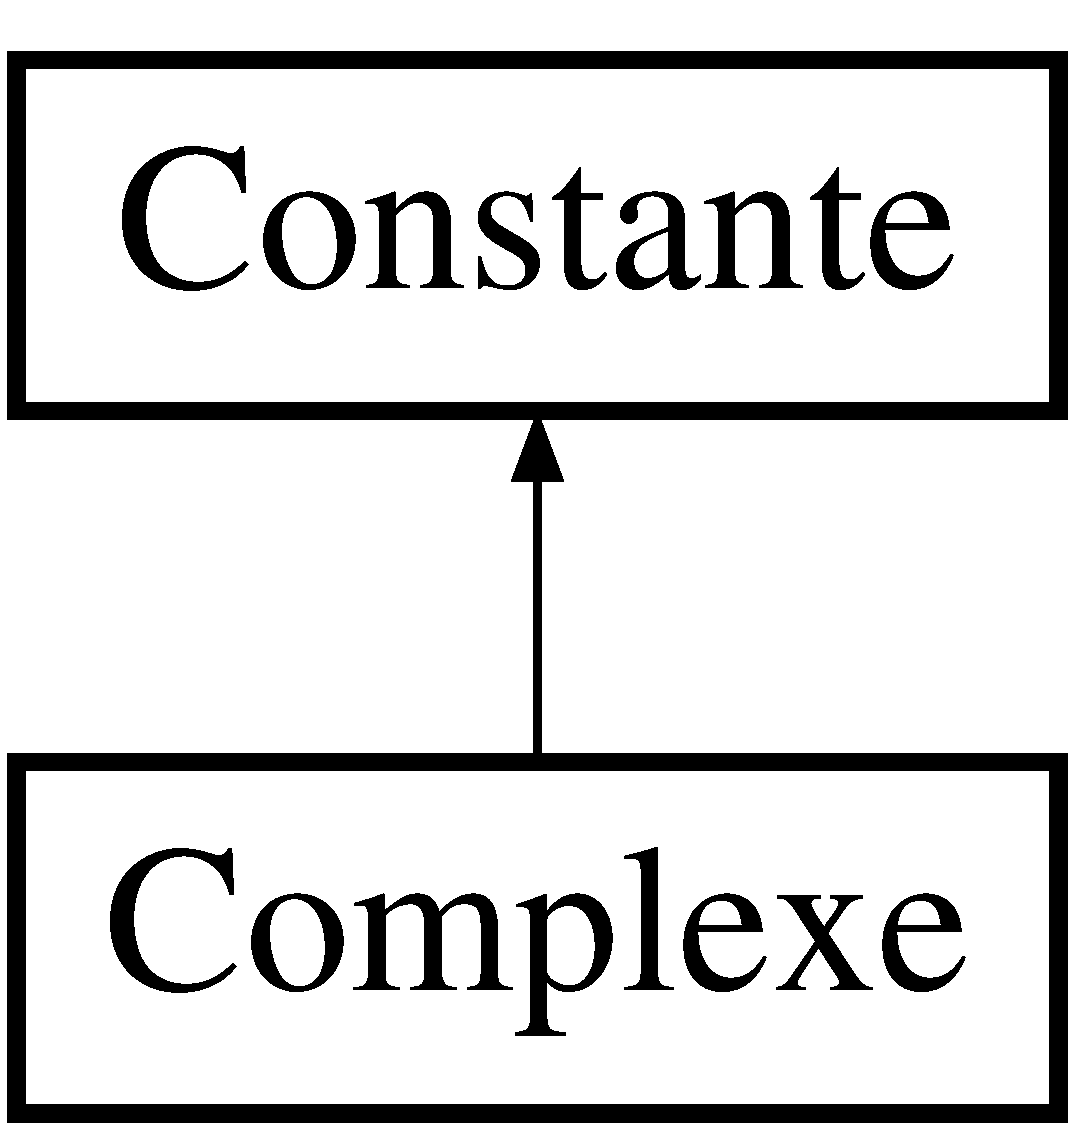
\includegraphics[height=2.000000cm]{class_complexe}
\end{center}
\end{figure}
\subsection*{Public Member Functions}
\begin{DoxyCompactItemize}
\item 
\hyperlink{class_complexe_a71a2f3b08ca8434c197ad8472afae798}{Complexe} (const std\-::string \&, const \hyperlink{constante_8h_a1d1cfd8ffb84e947f82999c682b666a7}{Type} \&)
\begin{DoxyCompactList}\small\item\em Constructeur. \end{DoxyCompactList}\item 
\hyperlink{class_complexe_a8863f7273658c9351d5b329b6cc48960}{Complexe} (const std\-::string \&val, const \hyperlink{constante_8h_a1d1cfd8ffb84e947f82999c682b666a7}{Type} \&T, const \hyperlink{constante_8h_a1d1cfd8ffb84e947f82999c682b666a7}{Type} \&Tvoulu, const \hyperlink{constante_8h_a1d1cfd8ffb84e947f82999c682b666a7}{Type} \&Torigine=\hyperlink{constante_8h_a1d1cfd8ffb84e947f82999c682b666a7a310a841612cf153caf2103c7d7136070}{entier})
\begin{DoxyCompactList}\small\item\em Constructeur. \end{DoxyCompactList}\item 
\hyperlink{class_complexe_a2148c05dc2027830c9464215d750f7cf}{Complexe} (const \hyperlink{class_complexe}{Complexe} \&)
\begin{DoxyCompactList}\small\item\em Constructeur de recopie. \end{DoxyCompactList}\item 
\hypertarget{class_complexe_ac92996231047d39d40e11384bb9311b6}{\hyperlink{class_complexe_ac92996231047d39d40e11384bb9311b6}{$\sim$\-Complexe} ()}\label{class_complexe_ac92996231047d39d40e11384bb9311b6}

\begin{DoxyCompactList}\small\item\em Destructeur. \end{DoxyCompactList}\item 
\hyperlink{class_constante}{Constante} $\ast$ \hyperlink{class_complexe_a5d1df6e75eb1c65b6c552a25d9810308}{get\-Reel} () const 
\begin{DoxyCompactList}\small\item\em Accesseur. \end{DoxyCompactList}\item 
\hyperlink{class_constante}{Constante} $\ast$ \hyperlink{class_complexe_a7e710082b1bf439beb9f1a49b49b8d2f}{get\-Im} () const 
\begin{DoxyCompactList}\small\item\em Accesseur. \end{DoxyCompactList}\item 
void \hyperlink{class_complexe_a677563f8839f7d4409bc6630feb12c45}{set\-Reel} (\hyperlink{class_constante}{Constante} $\ast$a)
\begin{DoxyCompactList}\small\item\em Accesseur. \end{DoxyCompactList}\item 
void \hyperlink{class_complexe_ab99400fbac2c12c03d8be8a38649e1ae}{set\-Im} (\hyperlink{class_constante}{Constante} $\ast$a)
\begin{DoxyCompactList}\small\item\em Accesseur. \end{DoxyCompactList}\item 
\hyperlink{constante_8h_a1d1cfd8ffb84e947f82999c682b666a7}{Type} \hyperlink{class_complexe_a2400a7038c5d98b3d85073dd5f56f415}{get\-\_\-complexe\-\_\-type\-\_\-contenu} () const 
\begin{DoxyCompactList}\small\item\em Accesseur. \end{DoxyCompactList}\item 
virtual std\-::string \hyperlink{class_complexe_a5eb44cf1cc373d1c2879c0c2de3d141a}{get\-Chain} () const 
\begin{DoxyCompactList}\small\item\em Accesseur. \end{DoxyCompactList}\item 
\hypertarget{class_complexe_a4fc1603f37056f0082ddc1517b60b7f7}{\hyperlink{class_complexe}{Complexe} \& \hyperlink{class_complexe_a4fc1603f37056f0082ddc1517b60b7f7}{operator+=} (\hyperlink{class_complexe}{Complexe} const \&e)}\label{class_complexe_a4fc1603f37056f0082ddc1517b60b7f7}

\begin{DoxyCompactList}\small\item\em Surcharge de +=. \end{DoxyCompactList}\item 
\hypertarget{class_complexe_a88a872cbf05d8228ce0ec068ab9371d8}{\hyperlink{class_complexe}{Complexe} \& \hyperlink{class_complexe_a88a872cbf05d8228ce0ec068ab9371d8}{operator-\/=} (\hyperlink{class_complexe}{Complexe} const \&e)}\label{class_complexe_a88a872cbf05d8228ce0ec068ab9371d8}

\begin{DoxyCompactList}\small\item\em Surcharge de -\/=. \end{DoxyCompactList}\item 
\hypertarget{class_complexe_a43bc434f00ede1a8c3ba29bc63b99ad8}{\hyperlink{class_complexe}{Complexe} \& \hyperlink{class_complexe_a43bc434f00ede1a8c3ba29bc63b99ad8}{operator$\ast$=} (\hyperlink{class_complexe}{Complexe} const \&e)}\label{class_complexe_a43bc434f00ede1a8c3ba29bc63b99ad8}

\begin{DoxyCompactList}\small\item\em Surcharge de $\ast$=. \end{DoxyCompactList}\item 
\hypertarget{class_complexe_a24bce7ffa93f0d6c1827925dcc919d7f}{\hyperlink{class_complexe}{Complexe} \& \hyperlink{class_complexe_a24bce7ffa93f0d6c1827925dcc919d7f}{operator/=} (\hyperlink{class_complexe}{Complexe} const \&e)}\label{class_complexe_a24bce7ffa93f0d6c1827925dcc919d7f}

\begin{DoxyCompactList}\small\item\em Surcharge de /=. \end{DoxyCompactList}\end{DoxyCompactItemize}
\subsection*{Private Member Functions}
\begin{DoxyCompactItemize}
\item 
virtual void \hyperlink{class_complexe_a7dd2fd72468a78b31fc2e95dfff8ee99}{build\-Constant} (const std\-::string \&)
\end{DoxyCompactItemize}
\subsection*{Private Attributes}
\begin{DoxyCompactItemize}
\item 
\hyperlink{class_constante}{Constante} $\ast$ \hyperlink{class_complexe_af2980d0c134931ec9b232a123e882bfe}{\-\_\-reel}
\item 
\hyperlink{class_constante}{Constante} $\ast$ \hyperlink{class_complexe_a8a3b2047469442fbe1e9c00cdeaa5c1a}{\-\_\-img}
\item 
\hyperlink{constante_8h_a1d1cfd8ffb84e947f82999c682b666a7}{Type} \hyperlink{class_complexe_a6c0cc92cd377b0b6f5dfd3bf8dceb961}{complexe\-\_\-type\-\_\-contenu}
\end{DoxyCompactItemize}


\subsection{Detailed Description}
classe definissant le type \hyperlink{class_complexe}{Complexe} herite de la classe \hyperlink{class_constante}{Constante} 

\subsection{Constructor \& Destructor Documentation}
\hypertarget{class_complexe_a71a2f3b08ca8434c197ad8472afae798}{\index{Complexe@{Complexe}!Complexe@{Complexe}}
\index{Complexe@{Complexe}!Complexe@{Complexe}}
\subsubsection[{Complexe}]{\setlength{\rightskip}{0pt plus 5cm}{\bf Complexe\-::\-Complexe} (
\begin{DoxyParamCaption}
\item[{const std\-::string \&}]{val, }
\item[{const {\bf Type} \&}]{T}
\end{DoxyParamCaption}
)}}\label{class_complexe_a71a2f3b08ca8434c197ad8472afae798}


Constructeur. 

Constructeur de la classe \hyperlink{class_complexe}{Complexe} initialisant le build\-Constante et le type du complexe 
\begin{DoxyParams}{Parameters}
{\em string} & \-: build\-Constante \\
\hline
{\em Type} & \-: Type \\
\hline
\end{DoxyParams}
\hypertarget{class_complexe_a8863f7273658c9351d5b329b6cc48960}{\index{Complexe@{Complexe}!Complexe@{Complexe}}
\index{Complexe@{Complexe}!Complexe@{Complexe}}
\subsubsection[{Complexe}]{\setlength{\rightskip}{0pt plus 5cm}{\bf Complexe\-::\-Complexe} (
\begin{DoxyParamCaption}
\item[{const std\-::string \&}]{val, }
\item[{const {\bf Type} \&}]{T, }
\item[{const {\bf Type} \&}]{Tvoulu, }
\item[{const {\bf Type} \&}]{Torigine = {\ttfamily {\bf entier}}}
\end{DoxyParamCaption}
)}}\label{class_complexe_a8863f7273658c9351d5b329b6cc48960}


Constructeur. 


\begin{DoxyParams}{Parameters}
{\em val} & \-: Texte r�cup�r� \\
\hline
{\em T} & \-: Type de val \\
\hline
{\em Tvoulu} & \-: Type du complexe que l'on souhaite obtenir \\
\hline
{\em Torigine} & \-: Type du complexe transmis \\
\hline
\end{DoxyParams}
\hypertarget{class_complexe_a2148c05dc2027830c9464215d750f7cf}{\index{Complexe@{Complexe}!Complexe@{Complexe}}
\index{Complexe@{Complexe}!Complexe@{Complexe}}
\subsubsection[{Complexe}]{\setlength{\rightskip}{0pt plus 5cm}{\bf Complexe\-::\-Complexe} (
\begin{DoxyParamCaption}
\item[{const {\bf Complexe} \&}]{a}
\end{DoxyParamCaption}
)}}\label{class_complexe_a2148c05dc2027830c9464215d750f7cf}


Constructeur de recopie. 


\begin{DoxyParams}{Parameters}
{\em \hyperlink{class_complexe}{Complexe}} & \-: \hyperlink{class_complexe}{Complexe} � copier dans le \hyperlink{class_complexe}{Complexe} pr�sent \\
\hline
\end{DoxyParams}


\subsection{Member Function Documentation}
\hypertarget{class_complexe_a7dd2fd72468a78b31fc2e95dfff8ee99}{\index{Complexe@{Complexe}!build\-Constant@{build\-Constant}}
\index{build\-Constant@{build\-Constant}!Complexe@{Complexe}}
\subsubsection[{build\-Constant}]{\setlength{\rightskip}{0pt plus 5cm}void {\bf Complexe\-::build\-Constant} (
\begin{DoxyParamCaption}
\item[{const std\-::string \&}]{val}
\end{DoxyParamCaption}
)\hspace{0.3cm}{\ttfamily  \mbox{[}private, virtual\mbox{]}}}}\label{class_complexe_a7dd2fd72468a78b31fc2e95dfff8ee99}
Constructeur de \hyperlink{class_constante}{Constante} empilable 

Implements \hyperlink{class_constante_afc5d0bb9363678d5b37543b5394c571e}{Constante}.

\hypertarget{class_complexe_a2400a7038c5d98b3d85073dd5f56f415}{\index{Complexe@{Complexe}!get\-\_\-complexe\-\_\-type\-\_\-contenu@{get\-\_\-complexe\-\_\-type\-\_\-contenu}}
\index{get\-\_\-complexe\-\_\-type\-\_\-contenu@{get\-\_\-complexe\-\_\-type\-\_\-contenu}!Complexe@{Complexe}}
\subsubsection[{get\-\_\-complexe\-\_\-type\-\_\-contenu}]{\setlength{\rightskip}{0pt plus 5cm}{\bf Type} {\bf Complexe\-::get\-\_\-complexe\-\_\-type\-\_\-contenu} (
\begin{DoxyParamCaption}
{}
\end{DoxyParamCaption}
) const\hspace{0.3cm}{\ttfamily  \mbox{[}inline\mbox{]}}}}\label{class_complexe_a2400a7038c5d98b3d85073dd5f56f415}


Accesseur. 

\begin{DoxyReturn}{Returns}
Type du contenu du complexe 
\end{DoxyReturn}
\hypertarget{class_complexe_a5eb44cf1cc373d1c2879c0c2de3d141a}{\index{Complexe@{Complexe}!get\-Chain@{get\-Chain}}
\index{get\-Chain@{get\-Chain}!Complexe@{Complexe}}
\subsubsection[{get\-Chain}]{\setlength{\rightskip}{0pt plus 5cm}std\-::string {\bf Complexe\-::get\-Chain} (
\begin{DoxyParamCaption}
{}
\end{DoxyParamCaption}
) const\hspace{0.3cm}{\ttfamily  \mbox{[}virtual\mbox{]}}}}\label{class_complexe_a5eb44cf1cc373d1c2879c0c2de3d141a}


Accesseur. 

\begin{DoxyReturn}{Returns}
La chaine correspondant au \hyperlink{class_complexe}{Complexe} 
\end{DoxyReturn}


Implements \hyperlink{class_constante_abd8a7f18b934053173ab87d947bd3386}{Constante}.

\hypertarget{class_complexe_a7e710082b1bf439beb9f1a49b49b8d2f}{\index{Complexe@{Complexe}!get\-Im@{get\-Im}}
\index{get\-Im@{get\-Im}!Complexe@{Complexe}}
\subsubsection[{get\-Im}]{\setlength{\rightskip}{0pt plus 5cm}{\bf Constante}$\ast$ {\bf Complexe\-::get\-Im} (
\begin{DoxyParamCaption}
{}
\end{DoxyParamCaption}
) const\hspace{0.3cm}{\ttfamily  \mbox{[}inline\mbox{]}}}}\label{class_complexe_a7e710082b1bf439beb9f1a49b49b8d2f}


Accesseur. 

\begin{DoxyReturn}{Returns}
Partie imaginaire 
\end{DoxyReturn}
\hypertarget{class_complexe_a5d1df6e75eb1c65b6c552a25d9810308}{\index{Complexe@{Complexe}!get\-Reel@{get\-Reel}}
\index{get\-Reel@{get\-Reel}!Complexe@{Complexe}}
\subsubsection[{get\-Reel}]{\setlength{\rightskip}{0pt plus 5cm}{\bf Constante}$\ast$ {\bf Complexe\-::get\-Reel} (
\begin{DoxyParamCaption}
{}
\end{DoxyParamCaption}
) const\hspace{0.3cm}{\ttfamily  \mbox{[}inline\mbox{]}}}}\label{class_complexe_a5d1df6e75eb1c65b6c552a25d9810308}


Accesseur. 

\begin{DoxyReturn}{Returns}
Partie r�elle 
\end{DoxyReturn}
\hypertarget{class_complexe_ab99400fbac2c12c03d8be8a38649e1ae}{\index{Complexe@{Complexe}!set\-Im@{set\-Im}}
\index{set\-Im@{set\-Im}!Complexe@{Complexe}}
\subsubsection[{set\-Im}]{\setlength{\rightskip}{0pt plus 5cm}void {\bf Complexe\-::set\-Im} (
\begin{DoxyParamCaption}
\item[{{\bf Constante} $\ast$}]{a}
\end{DoxyParamCaption}
)\hspace{0.3cm}{\ttfamily  \mbox{[}inline\mbox{]}}}}\label{class_complexe_ab99400fbac2c12c03d8be8a38649e1ae}


Accesseur. 

\begin{DoxyReturn}{Returns}
Modifie la partie imaginaire 
\end{DoxyReturn}
\hypertarget{class_complexe_a677563f8839f7d4409bc6630feb12c45}{\index{Complexe@{Complexe}!set\-Reel@{set\-Reel}}
\index{set\-Reel@{set\-Reel}!Complexe@{Complexe}}
\subsubsection[{set\-Reel}]{\setlength{\rightskip}{0pt plus 5cm}void {\bf Complexe\-::set\-Reel} (
\begin{DoxyParamCaption}
\item[{{\bf Constante} $\ast$}]{a}
\end{DoxyParamCaption}
)\hspace{0.3cm}{\ttfamily  \mbox{[}inline\mbox{]}}}}\label{class_complexe_a677563f8839f7d4409bc6630feb12c45}


Accesseur. 

\begin{DoxyReturn}{Returns}
Modifie la partie r�elle 
\end{DoxyReturn}


\subsection{Member Data Documentation}
\hypertarget{class_complexe_a8a3b2047469442fbe1e9c00cdeaa5c1a}{\index{Complexe@{Complexe}!\-\_\-img@{\-\_\-img}}
\index{\-\_\-img@{\-\_\-img}!Complexe@{Complexe}}
\subsubsection[{\-\_\-img}]{\setlength{\rightskip}{0pt plus 5cm}{\bf Constante}$\ast$ {\bf Complexe\-::\-\_\-img}\hspace{0.3cm}{\ttfamily  \mbox{[}private\mbox{]}}}}\label{class_complexe_a8a3b2047469442fbe1e9c00cdeaa5c1a}
Partie imaginaire \hypertarget{class_complexe_af2980d0c134931ec9b232a123e882bfe}{\index{Complexe@{Complexe}!\-\_\-reel@{\-\_\-reel}}
\index{\-\_\-reel@{\-\_\-reel}!Complexe@{Complexe}}
\subsubsection[{\-\_\-reel}]{\setlength{\rightskip}{0pt plus 5cm}{\bf Constante}$\ast$ {\bf Complexe\-::\-\_\-reel}\hspace{0.3cm}{\ttfamily  \mbox{[}private\mbox{]}}}}\label{class_complexe_af2980d0c134931ec9b232a123e882bfe}
Partie reelle \hypertarget{class_complexe_a6c0cc92cd377b0b6f5dfd3bf8dceb961}{\index{Complexe@{Complexe}!complexe\-\_\-type\-\_\-contenu@{complexe\-\_\-type\-\_\-contenu}}
\index{complexe\-\_\-type\-\_\-contenu@{complexe\-\_\-type\-\_\-contenu}!Complexe@{Complexe}}
\subsubsection[{complexe\-\_\-type\-\_\-contenu}]{\setlength{\rightskip}{0pt plus 5cm}{\bf Type} {\bf Complexe\-::complexe\-\_\-type\-\_\-contenu}\hspace{0.3cm}{\ttfamily  \mbox{[}private\mbox{]}}}}\label{class_complexe_a6c0cc92cd377b0b6f5dfd3bf8dceb961}
Type de contenu du complexe 

The documentation for this class was generated from the following files\-:\begin{DoxyCompactItemize}
\item 
\hyperlink{complexe_8h}{complexe.\-h}\item 
complexe.\-cpp\end{DoxyCompactItemize}

\hypertarget{class_constante}{\section{Constante Class Reference}
\label{class_constante}\index{Constante@{Constante}}
}


D�fini le type de \hyperlink{class_constante}{Constante}.  




{\ttfamily \#include $<$constante.\-h$>$}

Inheritance diagram for Constante\-:\begin{figure}[H]
\begin{center}
\leavevmode
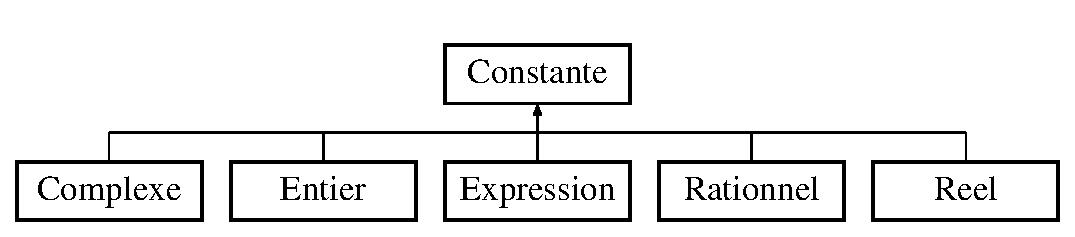
\includegraphics[height=2.000000cm]{class_constante}
\end{center}
\end{figure}
\subsection*{Public Member Functions}
\begin{DoxyCompactItemize}
\item 
const \hyperlink{constante_8h_a1d1cfd8ffb84e947f82999c682b666a7}{Type} \& \hyperlink{class_constante_ac259a3c2602b7b0132b62a7a6cb2c1d8}{get\-Type} ()
\begin{DoxyCompactList}\small\item\em Accesseur. \end{DoxyCompactList}\item 
virtual std\-::string \hyperlink{class_constante_abd8a7f18b934053173ab87d947bd3386}{get\-Chain} () const =0
\begin{DoxyCompactList}\small\item\em Accesseur. \end{DoxyCompactList}\end{DoxyCompactItemize}
\subsection*{Protected Member Functions}
\begin{DoxyCompactItemize}
\item 
virtual void \hyperlink{class_constante_afc5d0bb9363678d5b37543b5394c571e}{build\-Constant} (const std\-::string \&)=0
\end{DoxyCompactItemize}
\subsection*{Protected Attributes}
\begin{DoxyCompactItemize}
\item 
\hyperlink{constante_8h_a1d1cfd8ffb84e947f82999c682b666a7}{Type} \hyperlink{class_constante_a65ea08b29367b5189ff2a0f9146a87ff}{genre}
\end{DoxyCompactItemize}


\subsection{Detailed Description}
D�fini le type de \hyperlink{class_constante}{Constante}. 

\subsection{Member Function Documentation}
\hypertarget{class_constante_afc5d0bb9363678d5b37543b5394c571e}{\index{Constante@{Constante}!build\-Constant@{build\-Constant}}
\index{build\-Constant@{build\-Constant}!Constante@{Constante}}
\subsubsection[{build\-Constant}]{\setlength{\rightskip}{0pt plus 5cm}virtual void {\bf Constante\-::build\-Constant} (
\begin{DoxyParamCaption}
\item[{const std\-::string \&}]{}
\end{DoxyParamCaption}
)\hspace{0.3cm}{\ttfamily  \mbox{[}protected, pure virtual\mbox{]}}}}\label{class_constante_afc5d0bb9363678d5b37543b5394c571e}
Constructeur de constante empilable 

Implemented in \hyperlink{class_complexe_a7dd2fd72468a78b31fc2e95dfff8ee99}{Complexe}, \hyperlink{class_reel_a4b36b8926b60feedeb391dcdb7bb2e6e}{Reel}, \hyperlink{class_entier_ae45c94dab8160603b5c9f0ee0e0cc574}{Entier}, \hyperlink{class_expression_aefcd60203fbcab5f709aef85a0cd0323}{Expression}, and \hyperlink{class_rationnel_a3ee911afa5c5411814ab36b8cac948d7}{Rationnel}.

\hypertarget{class_constante_abd8a7f18b934053173ab87d947bd3386}{\index{Constante@{Constante}!get\-Chain@{get\-Chain}}
\index{get\-Chain@{get\-Chain}!Constante@{Constante}}
\subsubsection[{get\-Chain}]{\setlength{\rightskip}{0pt plus 5cm}virtual std\-::string {\bf Constante\-::get\-Chain} (
\begin{DoxyParamCaption}
{}
\end{DoxyParamCaption}
) const\hspace{0.3cm}{\ttfamily  \mbox{[}pure virtual\mbox{]}}}}\label{class_constante_abd8a7f18b934053173ab87d947bd3386}


Accesseur. 

\begin{DoxyReturn}{Returns}
La chaine correspondant � la \hyperlink{class_constante}{Constante} 
\end{DoxyReturn}


Implemented in \hyperlink{class_complexe_a5eb44cf1cc373d1c2879c0c2de3d141a}{Complexe}, \hyperlink{class_rationnel_ad9911305f668f4f537d541bb82e60a6b}{Rationnel}, \hyperlink{class_reel_aef757f3ab4b4fcea2b788fcafb10e8d1}{Reel}, \hyperlink{class_entier_a5c30af54c46b97d66bb88b36e255318c}{Entier}, and \hyperlink{class_expression_a9edab23bf777a9fc515719376d707aab}{Expression}.

\hypertarget{class_constante_ac259a3c2602b7b0132b62a7a6cb2c1d8}{\index{Constante@{Constante}!get\-Type@{get\-Type}}
\index{get\-Type@{get\-Type}!Constante@{Constante}}
\subsubsection[{get\-Type}]{\setlength{\rightskip}{0pt plus 5cm}const {\bf Type}\& {\bf Constante\-::get\-Type} (
\begin{DoxyParamCaption}
{}
\end{DoxyParamCaption}
)\hspace{0.3cm}{\ttfamily  \mbox{[}inline\mbox{]}}}}\label{class_constante_ac259a3c2602b7b0132b62a7a6cb2c1d8}


Accesseur. 

\begin{DoxyReturn}{Returns}
Le type de la \hyperlink{class_constante}{Constante} 
\end{DoxyReturn}


\subsection{Member Data Documentation}
\hypertarget{class_constante_a65ea08b29367b5189ff2a0f9146a87ff}{\index{Constante@{Constante}!genre@{genre}}
\index{genre@{genre}!Constante@{Constante}}
\subsubsection[{genre}]{\setlength{\rightskip}{0pt plus 5cm}{\bf Type} {\bf Constante\-::genre}\hspace{0.3cm}{\ttfamily  \mbox{[}protected\mbox{]}}}}\label{class_constante_a65ea08b29367b5189ff2a0f9146a87ff}
Type de la constante 

The documentation for this class was generated from the following file\-:\begin{DoxyCompactItemize}
\item 
\hyperlink{constante_8h}{constante.\-h}\end{DoxyCompactItemize}

\hypertarget{class_del_pile}{\section{Del\-Pile Class Reference}
\label{class_del_pile}\index{Del\-Pile@{Del\-Pile}}
}


Classe pour la gestion des suppressions sur la pile.  




{\ttfamily \#include $<$mainwindow.\-h$>$}

\subsection*{Public Member Functions}
\begin{DoxyCompactItemize}
\item 
\hypertarget{class_del_pile_a1fa3655064972bf31a88fd7cfa7c4b13}{\hyperlink{class_del_pile_a1fa3655064972bf31a88fd7cfa7c4b13}{Del\-Pile} (int i, Q\-Undo\-Command $\ast$parent=0)}\label{class_del_pile_a1fa3655064972bf31a88fd7cfa7c4b13}

\begin{DoxyCompactList}\small\item\em Constructeur de \hyperlink{class_del_pile}{Del\-Pile}. \end{DoxyCompactList}\item 
\hyperlink{class_constante}{Constante} $\ast$ \hyperlink{class_del_pile_aeedf15cdfe55a1251597c80108d32cf1}{get\-A} ()
\begin{DoxyCompactList}\small\item\em Accesseur. \end{DoxyCompactList}\item 
\hyperlink{class_constante}{Constante} $\ast$ \hyperlink{class_del_pile_ac57348b846881fd694ac43e1eefcdf38}{get\-B} ()
\begin{DoxyCompactList}\small\item\em Accesseur. \end{DoxyCompactList}\item 
\hypertarget{class_del_pile_a6eae5bd694d152a265e8acd3222632d9}{void \hyperlink{class_del_pile_a6eae5bd694d152a265e8acd3222632d9}{undo} ()}\label{class_del_pile_a6eae5bd694d152a265e8acd3222632d9}

\begin{DoxyCompactList}\small\item\em Empiler action inverse de la fonction \hyperlink{class_del_pile}{Del\-Pile}. \end{DoxyCompactList}\item 
\hypertarget{class_del_pile_a0af9499da3e8f72aacbb65f23b1c9b85}{void \hyperlink{class_del_pile_a0af9499da3e8f72aacbb65f23b1c9b85}{redo} ()}\label{class_del_pile_a0af9499da3e8f72aacbb65f23b1c9b85}

\begin{DoxyCompactList}\small\item\em D�piler action identique � la fonction \hyperlink{class_del_pile}{Del\-Pile}. \end{DoxyCompactList}\end{DoxyCompactItemize}
\subsection*{Private Attributes}
\begin{DoxyCompactItemize}
\item 
int \hyperlink{class_del_pile_a41c78904b2fdb15b5eb65675bfd7ed8a}{nb\-Const}
\item 
\hyperlink{class_constante}{Constante} $\ast$ \hyperlink{class_del_pile_abe7b2a46d1dc735e48721b461e51f537}{a}
\item 
\hyperlink{class_constante}{Constante} $\ast$ \hyperlink{class_del_pile_a7e87934f03f82947927f1417bc37ce0c}{b}
\end{DoxyCompactItemize}


\subsection{Detailed Description}
Classe pour la gestion des suppressions sur la pile. 

\subsection{Member Function Documentation}
\hypertarget{class_del_pile_aeedf15cdfe55a1251597c80108d32cf1}{\index{Del\-Pile@{Del\-Pile}!get\-A@{get\-A}}
\index{get\-A@{get\-A}!DelPile@{Del\-Pile}}
\subsubsection[{get\-A}]{\setlength{\rightskip}{0pt plus 5cm}{\bf Constante}$\ast$ {\bf Del\-Pile\-::get\-A} (
\begin{DoxyParamCaption}
{}
\end{DoxyParamCaption}
)\hspace{0.3cm}{\ttfamily  \mbox{[}inline\mbox{]}}}}\label{class_del_pile_aeedf15cdfe55a1251597c80108d32cf1}


Accesseur. 

\begin{DoxyReturn}{Returns}
Premi�re constante d�pil�e 
\end{DoxyReturn}
\hypertarget{class_del_pile_ac57348b846881fd694ac43e1eefcdf38}{\index{Del\-Pile@{Del\-Pile}!get\-B@{get\-B}}
\index{get\-B@{get\-B}!DelPile@{Del\-Pile}}
\subsubsection[{get\-B}]{\setlength{\rightskip}{0pt plus 5cm}{\bf Constante}$\ast$ {\bf Del\-Pile\-::get\-B} (
\begin{DoxyParamCaption}
{}
\end{DoxyParamCaption}
)\hspace{0.3cm}{\ttfamily  \mbox{[}inline\mbox{]}}}}\label{class_del_pile_ac57348b846881fd694ac43e1eefcdf38}


Accesseur. 

\begin{DoxyReturn}{Returns}
Deuxi�me constante d�pil�e 
\end{DoxyReturn}


\subsection{Member Data Documentation}
\hypertarget{class_del_pile_abe7b2a46d1dc735e48721b461e51f537}{\index{Del\-Pile@{Del\-Pile}!a@{a}}
\index{a@{a}!DelPile@{Del\-Pile}}
\subsubsection[{a}]{\setlength{\rightskip}{0pt plus 5cm}{\bf Constante}$\ast$ {\bf Del\-Pile\-::a}\hspace{0.3cm}{\ttfamily  \mbox{[}private\mbox{]}}}}\label{class_del_pile_abe7b2a46d1dc735e48721b461e51f537}
constante que l'on a supprim� de la pile \hypertarget{class_del_pile_a7e87934f03f82947927f1417bc37ce0c}{\index{Del\-Pile@{Del\-Pile}!b@{b}}
\index{b@{b}!DelPile@{Del\-Pile}}
\subsubsection[{b}]{\setlength{\rightskip}{0pt plus 5cm}{\bf Constante}$\ast$ {\bf Del\-Pile\-::b}\hspace{0.3cm}{\ttfamily  \mbox{[}private\mbox{]}}}}\label{class_del_pile_a7e87934f03f82947927f1417bc37ce0c}
constante que l'on a supprim� de la pile \hypertarget{class_del_pile_a41c78904b2fdb15b5eb65675bfd7ed8a}{\index{Del\-Pile@{Del\-Pile}!nb\-Const@{nb\-Const}}
\index{nb\-Const@{nb\-Const}!DelPile@{Del\-Pile}}
\subsubsection[{nb\-Const}]{\setlength{\rightskip}{0pt plus 5cm}int {\bf Del\-Pile\-::nb\-Const}\hspace{0.3cm}{\ttfamily  \mbox{[}private\mbox{]}}}}\label{class_del_pile_a41c78904b2fdb15b5eb65675bfd7ed8a}
nombre de constantes d�pil�es 

The documentation for this class was generated from the following files\-:\begin{DoxyCompactItemize}
\item 
\hyperlink{mainwindow_8h}{mainwindow.\-h}\item 
mainwindow.\-cpp\end{DoxyCompactItemize}

\hypertarget{class_del_texte}{\section{Del\-Texte Class Reference}
\label{class_del_texte}\index{Del\-Texte@{Del\-Texte}}
}


Classe pour la suppression de texte.  




{\ttfamily \#include $<$mainwindow.\-h$>$}

\subsection*{Public Member Functions}
\begin{DoxyCompactItemize}
\item 
\hypertarget{class_del_texte_abf47dea25e47cea3d57b09e4ce3ae8fe}{\hyperlink{class_del_texte_abf47dea25e47cea3d57b09e4ce3ae8fe}{Del\-Texte} (std\-::string s, \hyperlink{class_main_window}{Main\-Window} $\ast$w, Q\-Undo\-Command $\ast$parent=0)}\label{class_del_texte_abf47dea25e47cea3d57b09e4ce3ae8fe}

\begin{DoxyCompactList}\small\item\em Constructeur de \hyperlink{class_del_texte}{Del\-Texte}. \end{DoxyCompactList}\item 
\hypertarget{class_del_texte_a568b8313c7f7aa2268b5a3bd71431586}{void \hyperlink{class_del_texte_a568b8313c7f7aa2268b5a3bd71431586}{undo} ()}\label{class_del_texte_a568b8313c7f7aa2268b5a3bd71431586}

\begin{DoxyCompactList}\small\item\em Ajoute du texte de la \hyperlink{class_main_window}{Main\-Window} action inverse de la fonction \hyperlink{class_del_texte}{Del\-Texte}. \end{DoxyCompactList}\item 
\hypertarget{class_del_texte_a1a158b6a6f0bf877280e931bde93f832}{void \hyperlink{class_del_texte_a1a158b6a6f0bf877280e931bde93f832}{redo} ()}\label{class_del_texte_a1a158b6a6f0bf877280e931bde93f832}

\begin{DoxyCompactList}\small\item\em Efface du texte de la \hyperlink{class_main_window}{Main\-Window} action identique � la fonction \hyperlink{class_del_texte}{Del\-Texte}. \end{DoxyCompactList}\end{DoxyCompactItemize}
\subsection*{Private Attributes}
\begin{DoxyCompactItemize}
\item 
Q\-String \hyperlink{class_del_texte_a2760b6e7bd496f81117ebf7ae6c8bcaf}{chaine}
\item 
\hyperlink{class_main_window}{Main\-Window} $\ast$ \hyperlink{class_del_texte_afb19a55ac62c5c5ed67e73c9442ea88c}{ptr}
\end{DoxyCompactItemize}


\subsection{Detailed Description}
Classe pour la suppression de texte. 

\subsection{Member Data Documentation}
\hypertarget{class_del_texte_a2760b6e7bd496f81117ebf7ae6c8bcaf}{\index{Del\-Texte@{Del\-Texte}!chaine@{chaine}}
\index{chaine@{chaine}!DelTexte@{Del\-Texte}}
\subsubsection[{chaine}]{\setlength{\rightskip}{0pt plus 5cm}Q\-String {\bf Del\-Texte\-::chaine}\hspace{0.3cm}{\ttfamily  \mbox{[}private\mbox{]}}}}\label{class_del_texte_a2760b6e7bd496f81117ebf7ae6c8bcaf}
contenu de la chaine � supprimer \hypertarget{class_del_texte_afb19a55ac62c5c5ed67e73c9442ea88c}{\index{Del\-Texte@{Del\-Texte}!ptr@{ptr}}
\index{ptr@{ptr}!DelTexte@{Del\-Texte}}
\subsubsection[{ptr}]{\setlength{\rightskip}{0pt plus 5cm}{\bf Main\-Window}$\ast$ {\bf Del\-Texte\-::ptr}\hspace{0.3cm}{\ttfamily  \mbox{[}private\mbox{]}}}}\label{class_del_texte_afb19a55ac62c5c5ed67e73c9442ea88c}
la fenetre o� l'on va enlever le texte � supprimer 

The documentation for this class was generated from the following files\-:\begin{DoxyCompactItemize}
\item 
\hyperlink{mainwindow_8h}{mainwindow.\-h}\item 
mainwindow.\-cpp\end{DoxyCompactItemize}

\hypertarget{class_entier}{\section{Entier Class Reference}
\label{class_entier}\index{Entier@{Entier}}
}


D�fini le type \hyperlink{class_entier}{Entier} h�ritant de \hyperlink{class_constante}{Constante}.  




{\ttfamily \#include $<$entier.\-h$>$}

Inheritance diagram for Entier\-:\begin{figure}[H]
\begin{center}
\leavevmode
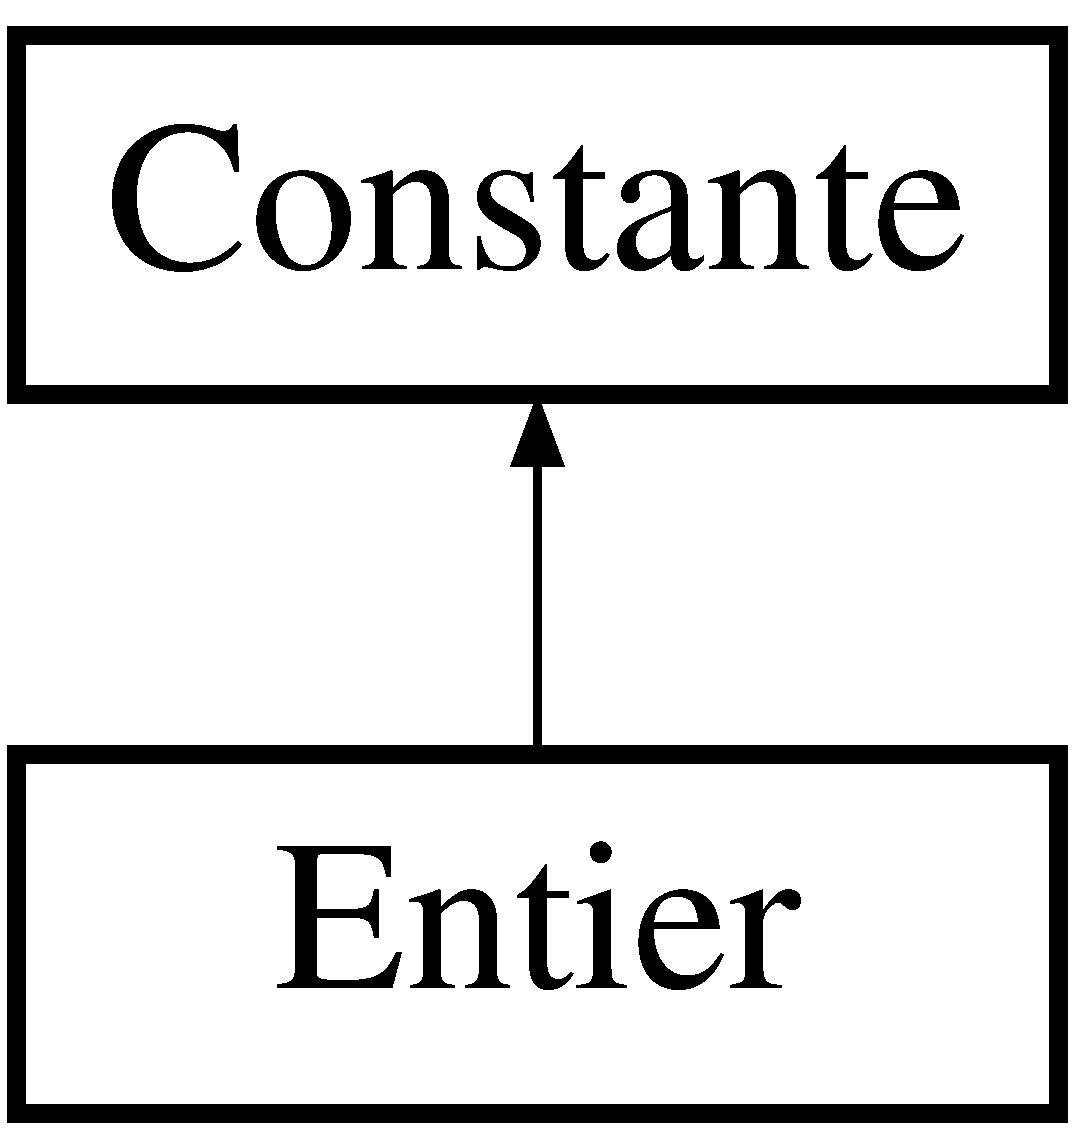
\includegraphics[height=2.000000cm]{class_entier}
\end{center}
\end{figure}
\subsection*{Public Member Functions}
\begin{DoxyCompactItemize}
\item 
\hyperlink{class_entier_a1479c4b87a60d4a7925553e242819ec3}{Entier} (const std\-::string \&val)
\begin{DoxyCompactList}\small\item\em Constructeur d'\hyperlink{class_entier}{Entier}. \end{DoxyCompactList}\item 
\hyperlink{class_entier_abcd2954e71be2bdc2e95fd2ae06bc250}{Entier} (const std\-::string \&val, const \hyperlink{constante_8h_a1d1cfd8ffb84e947f82999c682b666a7}{Type} \&T1, const \hyperlink{constante_8h_a1d1cfd8ffb84e947f82999c682b666a7}{Type} \&T2=\hyperlink{constante_8h_a1d1cfd8ffb84e947f82999c682b666a7a310a841612cf153caf2103c7d7136070}{entier})
\begin{DoxyCompactList}\small\item\em Constructeur. \end{DoxyCompactList}\item 
int \hyperlink{class_entier_ac6b87a29547b9814078220abb1b492fd}{get\-Val} () const 
\begin{DoxyCompactList}\small\item\em Accesseur. \end{DoxyCompactList}\item 
void \hyperlink{class_entier_a70732595b8d42a97a5852d64409bed80}{set\-Val} (const int \&i)
\begin{DoxyCompactList}\small\item\em Accesseur. \end{DoxyCompactList}\item 
virtual std\-::string \hyperlink{class_entier_a5c30af54c46b97d66bb88b36e255318c}{get\-Chain} () const 
\begin{DoxyCompactList}\small\item\em Accesseur. \end{DoxyCompactList}\item 
\hypertarget{class_entier_a64bb8c91174b8681aeda6768bac10092}{\hyperlink{class_entier}{Entier} \& \hyperlink{class_entier_a64bb8c91174b8681aeda6768bac10092}{operator+=} (\hyperlink{class_entier}{Entier} const \&e)}\label{class_entier_a64bb8c91174b8681aeda6768bac10092}

\begin{DoxyCompactList}\small\item\em Surrcharge de +=. \end{DoxyCompactList}\item 
\hypertarget{class_entier_a951a672d44c981f78b52c483c7afd999}{\hyperlink{class_entier}{Entier} \& \hyperlink{class_entier_a951a672d44c981f78b52c483c7afd999}{operator-\/=} (\hyperlink{class_entier}{Entier} const \&e)}\label{class_entier_a951a672d44c981f78b52c483c7afd999}

\begin{DoxyCompactList}\small\item\em Surrcharge de -\/=. \end{DoxyCompactList}\item 
\hypertarget{class_entier_ab738bbac9f96c1745f709c42f41df76e}{\hyperlink{class_entier}{Entier} \& \hyperlink{class_entier_ab738bbac9f96c1745f709c42f41df76e}{operator$\ast$=} (\hyperlink{class_entier}{Entier} const \&e)}\label{class_entier_ab738bbac9f96c1745f709c42f41df76e}

\begin{DoxyCompactList}\small\item\em Surrcharge de $\ast$=. \end{DoxyCompactList}\item 
\hypertarget{class_entier_ae85beca57d573908e13d7c6110d665e2}{\hyperlink{class_entier}{Entier} \& \hyperlink{class_entier_ae85beca57d573908e13d7c6110d665e2}{operator/=} (\hyperlink{class_entier}{Entier} const \&e)}\label{class_entier_ae85beca57d573908e13d7c6110d665e2}

\begin{DoxyCompactList}\small\item\em Surrcharge de /=. \end{DoxyCompactList}\end{DoxyCompactItemize}
\subsection*{Private Member Functions}
\begin{DoxyCompactItemize}
\item 
virtual void \hyperlink{class_entier_ae45c94dab8160603b5c9f0ee0e0cc574}{build\-Constant} (const std\-::string \&)
\end{DoxyCompactItemize}
\subsection*{Private Attributes}
\begin{DoxyCompactItemize}
\item 
int \hyperlink{class_entier_a90524161dcd75977cb36a7eb5d42f627}{valeur}
\end{DoxyCompactItemize}


\subsection{Detailed Description}
D�fini le type \hyperlink{class_entier}{Entier} h�ritant de \hyperlink{class_constante}{Constante}. 

\subsection{Constructor \& Destructor Documentation}
\hypertarget{class_entier_a1479c4b87a60d4a7925553e242819ec3}{\index{Entier@{Entier}!Entier@{Entier}}
\index{Entier@{Entier}!Entier@{Entier}}
\subsubsection[{Entier}]{\setlength{\rightskip}{0pt plus 5cm}{\bf Entier\-::\-Entier} (
\begin{DoxyParamCaption}
\item[{const std\-::string \&}]{val}
\end{DoxyParamCaption}
)}}\label{class_entier_a1479c4b87a60d4a7925553e242819ec3}


Constructeur d'\hyperlink{class_entier}{Entier}. 


\begin{DoxyParams}{Parameters}
{\em val} & \-: Chaine de caract�re initialisant l'\hyperlink{class_entier}{Entier} \\
\hline
\end{DoxyParams}
\hypertarget{class_entier_abcd2954e71be2bdc2e95fd2ae06bc250}{\index{Entier@{Entier}!Entier@{Entier}}
\index{Entier@{Entier}!Entier@{Entier}}
\subsubsection[{Entier}]{\setlength{\rightskip}{0pt plus 5cm}{\bf Entier\-::\-Entier} (
\begin{DoxyParamCaption}
\item[{const std\-::string \&}]{val, }
\item[{const {\bf Type} \&}]{T1, }
\item[{const {\bf Type} \&}]{T2 = {\ttfamily {\bf entier}}}
\end{DoxyParamCaption}
)}}\label{class_entier_abcd2954e71be2bdc2e95fd2ae06bc250}


Constructeur. 


\begin{DoxyParams}{Parameters}
{\em val} & \-: Texte r�cup�r� \\
\hline
{\em T1} & \-: Type de val \\
\hline
{\em T2} & \-: Type du complexe que l'on souhaite obtenir \\
\hline
\end{DoxyParams}


\subsection{Member Function Documentation}
\hypertarget{class_entier_ae45c94dab8160603b5c9f0ee0e0cc574}{\index{Entier@{Entier}!build\-Constant@{build\-Constant}}
\index{build\-Constant@{build\-Constant}!Entier@{Entier}}
\subsubsection[{build\-Constant}]{\setlength{\rightskip}{0pt plus 5cm}void {\bf Entier\-::build\-Constant} (
\begin{DoxyParamCaption}
\item[{const std\-::string \&}]{val}
\end{DoxyParamCaption}
)\hspace{0.3cm}{\ttfamily  \mbox{[}private, virtual\mbox{]}}}}\label{class_entier_ae45c94dab8160603b5c9f0ee0e0cc574}
Constructeur de constante empilable 

Implements \hyperlink{class_constante_afc5d0bb9363678d5b37543b5394c571e}{Constante}.

\hypertarget{class_entier_a5c30af54c46b97d66bb88b36e255318c}{\index{Entier@{Entier}!get\-Chain@{get\-Chain}}
\index{get\-Chain@{get\-Chain}!Entier@{Entier}}
\subsubsection[{get\-Chain}]{\setlength{\rightskip}{0pt plus 5cm}std\-::string {\bf Entier\-::get\-Chain} (
\begin{DoxyParamCaption}
{}
\end{DoxyParamCaption}
) const\hspace{0.3cm}{\ttfamily  \mbox{[}virtual\mbox{]}}}}\label{class_entier_a5c30af54c46b97d66bb88b36e255318c}


Accesseur. 

\begin{DoxyReturn}{Returns}
Renvoi la chaine correspondant � l'\hyperlink{class_entier}{Entier} 
\end{DoxyReturn}


Implements \hyperlink{class_constante_abd8a7f18b934053173ab87d947bd3386}{Constante}.

\hypertarget{class_entier_ac6b87a29547b9814078220abb1b492fd}{\index{Entier@{Entier}!get\-Val@{get\-Val}}
\index{get\-Val@{get\-Val}!Entier@{Entier}}
\subsubsection[{get\-Val}]{\setlength{\rightskip}{0pt plus 5cm}int {\bf Entier\-::get\-Val} (
\begin{DoxyParamCaption}
{}
\end{DoxyParamCaption}
) const\hspace{0.3cm}{\ttfamily  \mbox{[}inline\mbox{]}}}}\label{class_entier_ac6b87a29547b9814078220abb1b492fd}


Accesseur. 

\begin{DoxyReturn}{Returns}
L'\hyperlink{class_entier}{Entier} 
\end{DoxyReturn}
\hypertarget{class_entier_a70732595b8d42a97a5852d64409bed80}{\index{Entier@{Entier}!set\-Val@{set\-Val}}
\index{set\-Val@{set\-Val}!Entier@{Entier}}
\subsubsection[{set\-Val}]{\setlength{\rightskip}{0pt plus 5cm}void {\bf Entier\-::set\-Val} (
\begin{DoxyParamCaption}
\item[{const int \&}]{i}
\end{DoxyParamCaption}
)\hspace{0.3cm}{\ttfamily  \mbox{[}inline\mbox{]}}}}\label{class_entier_a70732595b8d42a97a5852d64409bed80}


Accesseur. 

modifie l'\hyperlink{class_entier}{Entier} 

\subsection{Member Data Documentation}
\hypertarget{class_entier_a90524161dcd75977cb36a7eb5d42f627}{\index{Entier@{Entier}!valeur@{valeur}}
\index{valeur@{valeur}!Entier@{Entier}}
\subsubsection[{valeur}]{\setlength{\rightskip}{0pt plus 5cm}int {\bf Entier\-::valeur}\hspace{0.3cm}{\ttfamily  \mbox{[}private\mbox{]}}}}\label{class_entier_a90524161dcd75977cb36a7eb5d42f627}
L'entier 

The documentation for this class was generated from the following files\-:\begin{DoxyCompactItemize}
\item 
\hyperlink{entier_8h}{entier.\-h}\item 
entier.\-cpp\end{DoxyCompactItemize}

\hypertarget{class_expression}{\section{Expression Class Reference}
\label{class_expression}\index{Expression@{Expression}}
}


classe definissant le type \hyperlink{class_expression}{Expression}, herite de la classe \hyperlink{class_constante}{Constante}  




{\ttfamily \#include $<$expression.\-h$>$}

Inheritance diagram for Expression\-:\begin{figure}[H]
\begin{center}
\leavevmode
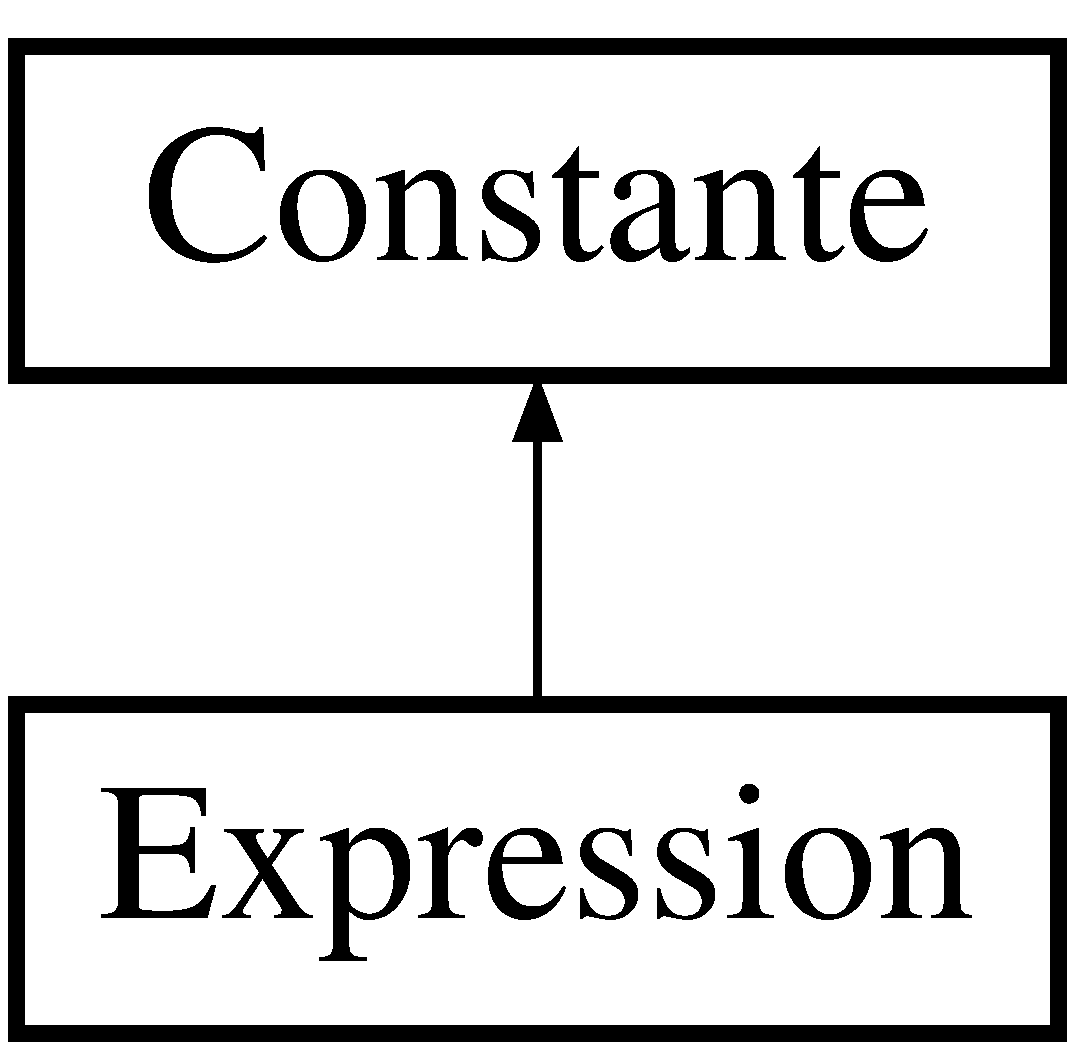
\includegraphics[height=2.000000cm]{class_expression}
\end{center}
\end{figure}
\subsection*{Public Member Functions}
\begin{DoxyCompactItemize}
\item 
\hyperlink{class_expression_a38fbd99c8fcd7b00fbdad260523e0e3b}{Expression} (std\-::string const \&val)
\begin{DoxyCompactList}\small\item\em Constructeur \hyperlink{class_expression}{Expression} initiallis�e avec un string. \end{DoxyCompactList}\item 
std\-::string \hyperlink{class_expression_a2c596d0bcddba04fef7340e41593f2ca}{get\-Expr} () const 
\begin{DoxyCompactList}\small\item\em Accesseur. \end{DoxyCompactList}\item 
\hypertarget{class_expression_ace99c09f6dc00d79a81177f62e0e39ba}{void \hyperlink{class_expression_ace99c09f6dc00d79a81177f62e0e39ba}{set\-Expr} (const std\-::string \&s)}\label{class_expression_ace99c09f6dc00d79a81177f62e0e39ba}

\begin{DoxyCompactList}\small\item\em Accesseur Change la valeur de l'\hyperlink{class_expression}{Expression}. \end{DoxyCompactList}\item 
virtual std\-::string \hyperlink{class_expression_a9edab23bf777a9fc515719376d707aab}{get\-Chain} () const 
\begin{DoxyCompactList}\small\item\em Chaine de l'\hyperlink{class_expression}{Expression}. \end{DoxyCompactList}\end{DoxyCompactItemize}
\subsection*{Private Member Functions}
\begin{DoxyCompactItemize}
\item 
void \hyperlink{class_expression_aefcd60203fbcab5f709aef85a0cd0323}{build\-Constant} (const std\-::string \&val)
\end{DoxyCompactItemize}
\subsection*{Private Attributes}
\begin{DoxyCompactItemize}
\item 
std\-::string \hyperlink{class_expression_a22cd0226f850627647051c4e2ca97891}{expr}
\end{DoxyCompactItemize}


\subsection{Detailed Description}
classe definissant le type \hyperlink{class_expression}{Expression}, herite de la classe \hyperlink{class_constante}{Constante} 

\subsection{Constructor \& Destructor Documentation}
\hypertarget{class_expression_a38fbd99c8fcd7b00fbdad260523e0e3b}{\index{Expression@{Expression}!Expression@{Expression}}
\index{Expression@{Expression}!Expression@{Expression}}
\subsubsection[{Expression}]{\setlength{\rightskip}{0pt plus 5cm}{\bf Expression\-::\-Expression} (
\begin{DoxyParamCaption}
\item[{std\-::string const \&}]{val}
\end{DoxyParamCaption}
)}}\label{class_expression_a38fbd99c8fcd7b00fbdad260523e0e3b}


Constructeur \hyperlink{class_expression}{Expression} initiallis�e avec un string. 


\begin{DoxyParams}{Parameters}
{\em val} & \-: La nouvelle \hyperlink{class_expression}{Expression} \\
\hline
\end{DoxyParams}


\subsection{Member Function Documentation}
\hypertarget{class_expression_aefcd60203fbcab5f709aef85a0cd0323}{\index{Expression@{Expression}!build\-Constant@{build\-Constant}}
\index{build\-Constant@{build\-Constant}!Expression@{Expression}}
\subsubsection[{build\-Constant}]{\setlength{\rightskip}{0pt plus 5cm}void {\bf Expression\-::build\-Constant} (
\begin{DoxyParamCaption}
\item[{const std\-::string \&}]{val}
\end{DoxyParamCaption}
)\hspace{0.3cm}{\ttfamily  \mbox{[}private, virtual\mbox{]}}}}\label{class_expression_aefcd60203fbcab5f709aef85a0cd0323}
Constructeur de \hyperlink{class_constante}{Constante} empilable 

Implements \hyperlink{class_constante_afc5d0bb9363678d5b37543b5394c571e}{Constante}.

\hypertarget{class_expression_a9edab23bf777a9fc515719376d707aab}{\index{Expression@{Expression}!get\-Chain@{get\-Chain}}
\index{get\-Chain@{get\-Chain}!Expression@{Expression}}
\subsubsection[{get\-Chain}]{\setlength{\rightskip}{0pt plus 5cm}std\-::string {\bf Expression\-::get\-Chain} (
\begin{DoxyParamCaption}
{}
\end{DoxyParamCaption}
) const\hspace{0.3cm}{\ttfamily  \mbox{[}virtual\mbox{]}}}}\label{class_expression_a9edab23bf777a9fc515719376d707aab}


Chaine de l'\hyperlink{class_expression}{Expression}. 

\begin{DoxyReturn}{Returns}
la chaine correspondant � l'\hyperlink{class_expression}{Expression} 
\end{DoxyReturn}


Implements \hyperlink{class_constante_abd8a7f18b934053173ab87d947bd3386}{Constante}.

\hypertarget{class_expression_a2c596d0bcddba04fef7340e41593f2ca}{\index{Expression@{Expression}!get\-Expr@{get\-Expr}}
\index{get\-Expr@{get\-Expr}!Expression@{Expression}}
\subsubsection[{get\-Expr}]{\setlength{\rightskip}{0pt plus 5cm}std\-::string {\bf Expression\-::get\-Expr} (
\begin{DoxyParamCaption}
{}
\end{DoxyParamCaption}
) const\hspace{0.3cm}{\ttfamily  \mbox{[}inline\mbox{]}}}}\label{class_expression_a2c596d0bcddba04fef7340e41593f2ca}


Accesseur. 

\begin{DoxyReturn}{Returns}
L'\hyperlink{class_expression}{Expression} 
\end{DoxyReturn}


\subsection{Member Data Documentation}
\hypertarget{class_expression_a22cd0226f850627647051c4e2ca97891}{\index{Expression@{Expression}!expr@{expr}}
\index{expr@{expr}!Expression@{Expression}}
\subsubsection[{expr}]{\setlength{\rightskip}{0pt plus 5cm}std\-::string {\bf Expression\-::expr}\hspace{0.3cm}{\ttfamily  \mbox{[}private\mbox{]}}}}\label{class_expression_a22cd0226f850627647051c4e2ca97891}
L'expression 

The documentation for this class was generated from the following files\-:\begin{DoxyCompactItemize}
\item 
\hyperlink{expression_8h}{expression.\-h}\item 
expression.\-cpp\end{DoxyCompactItemize}

\hypertarget{class_factory_const}{\section{Factory\-Const Class Reference}
\label{class_factory_const}\index{Factory\-Const@{Factory\-Const}}
}


{\ttfamily \#include $<$factoryconst.\-h$>$}

\subsection*{Static Public Member Functions}
\begin{DoxyCompactItemize}
\item 
static \hyperlink{class_constante}{Constante} $\ast$ \hyperlink{class_factory_const_a6d3d775f9c3c3588dad86e51c04a1a22}{create\-Constant} (const std\-::string \&val, const \hyperlink{constante_8h_a1d1cfd8ffb84e947f82999c682b666a7}{Type} \&T)
\begin{DoxyCompactList}\small\item\em Cr�� une constante. \end{DoxyCompactList}\item 
static \hyperlink{class_constante}{Constante} $\ast$ \hyperlink{class_factory_const_ac84334f8ef4b8f5e91df5826a3773e9d}{create\-Constant} (const std\-::string \&val, const \hyperlink{constante_8h_a1d1cfd8ffb84e947f82999c682b666a7}{Type} \&T, const \hyperlink{constante_8h_a1d1cfd8ffb84e947f82999c682b666a7}{Type} \&Tdonne)
\begin{DoxyCompactList}\small\item\em Cr�� une constante. \end{DoxyCompactList}\item 
static \hyperlink{class_constante}{Constante} $\ast$ \hyperlink{class_factory_const_ab0d818c4a2b6303a0317272623f06098}{create\-Constant} (const std\-::string \&val, const \hyperlink{constante_8h_a1d1cfd8ffb84e947f82999c682b666a7}{Type} \&T, const \hyperlink{constante_8h_a1d1cfd8ffb84e947f82999c682b666a7}{Type} \&Tdonne, const \hyperlink{constante_8h_a1d1cfd8ffb84e947f82999c682b666a7}{Type} \&Tcomplexe)
\begin{DoxyCompactList}\small\item\em Cr�� une constante. \end{DoxyCompactList}\item 
static \hyperlink{class_constante}{Constante} $\ast$ \hyperlink{class_factory_const_a40d3b4a8e521b3b31e5e79a9a40a395b}{create\-Constant} (const std\-::string \&val, const \hyperlink{constante_8h_a1d1cfd8ffb84e947f82999c682b666a7}{Type} \&T, const \hyperlink{constante_8h_a1d1cfd8ffb84e947f82999c682b666a7}{Type} \&Tdonne, const \hyperlink{constante_8h_a1d1cfd8ffb84e947f82999c682b666a7}{Type} \&Tvoulu, const \hyperlink{constante_8h_a1d1cfd8ffb84e947f82999c682b666a7}{Type} \&Torigine)
\begin{DoxyCompactList}\small\item\em Cr�� une constante. \end{DoxyCompactList}\end{DoxyCompactItemize}
\subsection*{Private Member Functions}
\begin{DoxyCompactItemize}
\item 
\hypertarget{class_factory_const_ad1c7249e08797806ba7c3b4c11dee152}{\hyperlink{class_factory_const_ad1c7249e08797806ba7c3b4c11dee152}{Factory\-Const} ()}\label{class_factory_const_ad1c7249e08797806ba7c3b4c11dee152}

\begin{DoxyCompactList}\small\item\em Constructeur Empeche toute instanciation de \hyperlink{class_factory_const}{Factory\-Const}. \end{DoxyCompactList}\end{DoxyCompactItemize}


\subsection{Detailed Description}
Cr�� des constante depuis les types strings retourn� par les diff�rentes constantes 

\subsection{Member Function Documentation}
\hypertarget{class_factory_const_a6d3d775f9c3c3588dad86e51c04a1a22}{\index{Factory\-Const@{Factory\-Const}!create\-Constant@{create\-Constant}}
\index{create\-Constant@{create\-Constant}!FactoryConst@{Factory\-Const}}
\subsubsection[{create\-Constant}]{\setlength{\rightskip}{0pt plus 5cm}{\bf Constante} $\ast$ {\bf Factory\-Const\-::create\-Constant} (
\begin{DoxyParamCaption}
\item[{const std\-::string \&}]{val, }
\item[{const {\bf Type} \&}]{T}
\end{DoxyParamCaption}
)\hspace{0.3cm}{\ttfamily  \mbox{[}static\mbox{]}}}}\label{class_factory_const_a6d3d775f9c3c3588dad86e51c04a1a22}


Cr�� une constante. 


\begin{DoxyParams}{Parameters}
{\em val} & \-: la valeur pr�c�dement convertie en string \\
\hline
{\em T} & \-: Type de val \\
\hline
\end{DoxyParams}
\begin{DoxyReturn}{Returns}
\hyperlink{class_constante}{Constante} de type T 
\end{DoxyReturn}
\hypertarget{class_factory_const_ac84334f8ef4b8f5e91df5826a3773e9d}{\index{Factory\-Const@{Factory\-Const}!create\-Constant@{create\-Constant}}
\index{create\-Constant@{create\-Constant}!FactoryConst@{Factory\-Const}}
\subsubsection[{create\-Constant}]{\setlength{\rightskip}{0pt plus 5cm}{\bf Constante} $\ast$ {\bf Factory\-Const\-::create\-Constant} (
\begin{DoxyParamCaption}
\item[{const std\-::string \&}]{val, }
\item[{const {\bf Type} \&}]{T, }
\item[{const {\bf Type} \&}]{Tdonne}
\end{DoxyParamCaption}
)\hspace{0.3cm}{\ttfamily  \mbox{[}static\mbox{]}}}}\label{class_factory_const_ac84334f8ef4b8f5e91df5826a3773e9d}


Cr�� une constante. 


\begin{DoxyParams}{Parameters}
{\em val} & \-: la valeur pr�c�dement convertie en string \\
\hline
{\em T} & \-: Type de val \\
\hline
{\em Tdonne} & \-: Type voulu en retour \\
\hline
\end{DoxyParams}
\begin{DoxyReturn}{Returns}
\hyperlink{class_constante}{Constante} de type Tdonne 
\end{DoxyReturn}
\hypertarget{class_factory_const_ab0d818c4a2b6303a0317272623f06098}{\index{Factory\-Const@{Factory\-Const}!create\-Constant@{create\-Constant}}
\index{create\-Constant@{create\-Constant}!FactoryConst@{Factory\-Const}}
\subsubsection[{create\-Constant}]{\setlength{\rightskip}{0pt plus 5cm}{\bf Constante} $\ast$ {\bf Factory\-Const\-::create\-Constant} (
\begin{DoxyParamCaption}
\item[{const std\-::string \&}]{val, }
\item[{const {\bf Type} \&}]{T, }
\item[{const {\bf Type} \&}]{Tdonne, }
\item[{const {\bf Type} \&}]{Tcomplexe}
\end{DoxyParamCaption}
)\hspace{0.3cm}{\ttfamily  \mbox{[}static\mbox{]}}}}\label{class_factory_const_ab0d818c4a2b6303a0317272623f06098}


Cr�� une constante. 


\begin{DoxyParams}{Parameters}
{\em val} & \-: la valeur pr�c�dement convertie en string \\
\hline
{\em T} & \-: Type de val \\
\hline
{\em Tdonne} & \-: Type voulu en retour \\
\hline
{\em Tcomplexe} & \-: Type des parties r�elles et imaginaires du complexe \\
\hline
\end{DoxyParams}
\begin{DoxyReturn}{Returns}
\hyperlink{class_constante}{Constante} de type Tdonne 
\end{DoxyReturn}
\hypertarget{class_factory_const_a40d3b4a8e521b3b31e5e79a9a40a395b}{\index{Factory\-Const@{Factory\-Const}!create\-Constant@{create\-Constant}}
\index{create\-Constant@{create\-Constant}!FactoryConst@{Factory\-Const}}
\subsubsection[{create\-Constant}]{\setlength{\rightskip}{0pt plus 5cm}{\bf Constante} $\ast$ {\bf Factory\-Const\-::create\-Constant} (
\begin{DoxyParamCaption}
\item[{const std\-::string \&}]{val, }
\item[{const {\bf Type} \&}]{T, }
\item[{const {\bf Type} \&}]{Tdonne, }
\item[{const {\bf Type} \&}]{Tvoulu, }
\item[{const {\bf Type} \&}]{Torigine}
\end{DoxyParamCaption}
)\hspace{0.3cm}{\ttfamily  \mbox{[}static\mbox{]}}}}\label{class_factory_const_a40d3b4a8e521b3b31e5e79a9a40a395b}


Cr�� une constante. 


\begin{DoxyParams}{Parameters}
{\em val} & \-: la valeur pr�c�dement convertie en string \\
\hline
{\em T} & \-: Type de val \\
\hline
{\em Tdonne} & \-: Type voulu en retour \\
\hline
{\em Tvoulu} & \-: Type voulu pour le complexe \\
\hline
{\em Torigine} & \-: Type d'origine du complexe \\
\hline
\end{DoxyParams}
\begin{DoxyReturn}{Returns}
\hyperlink{class_constante}{Constante} de type Tdonne 
\end{DoxyReturn}


The documentation for this class was generated from the following files\-:\begin{DoxyCompactItemize}
\item 
\hyperlink{factoryconst_8h}{factoryconst.\-h}\item 
factoryconst.\-cpp\end{DoxyCompactItemize}

\hypertarget{class_log_message}{\section{Log\-Message Class Reference}
\label{class_log_message}\index{Log\-Message@{Log\-Message}}
}


Classe pour les messages log.  




{\ttfamily \#include $<$logsystem.\-h$>$}

\subsection*{Public Member Functions}
\begin{DoxyCompactItemize}
\item 
\hyperlink{class_log_message_a4f09753304180179419558a4ba145f8e}{Log\-Message} (const std\-::string \&, unsigned int)
\begin{DoxyCompactList}\small\item\em Constructeur. \end{DoxyCompactList}\item 
\hypertarget{class_log_message_a0197adf0d9ba3c1af36e538467bfb9b1}{Q\-String \hyperlink{class_log_message_a0197adf0d9ba3c1af36e538467bfb9b1}{get\-Log} () const }\label{class_log_message_a0197adf0d9ba3c1af36e538467bfb9b1}

\begin{DoxyCompactList}\small\item\em Partie du message pr�cisant le degr� d'importance du message. \end{DoxyCompactList}\end{DoxyCompactItemize}
\subsection*{Private Attributes}
\begin{DoxyCompactItemize}
\item 
Q\-String \hyperlink{class_log_message_ac9a5fe391cd0eab2a87a6788cb6b658b}{log}
\item 
unsigned int \hyperlink{class_log_message_ae7ca7402697ca5fa97c7892b47ee7f47}{degree}
\end{DoxyCompactItemize}


\subsection{Detailed Description}
Classe pour les messages log. 

\subsection{Constructor \& Destructor Documentation}
\hypertarget{class_log_message_a4f09753304180179419558a4ba145f8e}{\index{Log\-Message@{Log\-Message}!Log\-Message@{Log\-Message}}
\index{Log\-Message@{Log\-Message}!LogMessage@{Log\-Message}}
\subsubsection[{Log\-Message}]{\setlength{\rightskip}{0pt plus 5cm}{\bf Log\-Message\-::\-Log\-Message} (
\begin{DoxyParamCaption}
\item[{const std\-::string \&}]{s, }
\item[{unsigned int}]{i}
\end{DoxyParamCaption}
)}}\label{class_log_message_a4f09753304180179419558a4ba145f8e}


Constructeur. 


\begin{DoxyParams}{Parameters}
{\em Contenu} & du message \\
\hline
{\em Degre} & d'importance du message \\
\hline
\end{DoxyParams}


\subsection{Member Data Documentation}
\hypertarget{class_log_message_ae7ca7402697ca5fa97c7892b47ee7f47}{\index{Log\-Message@{Log\-Message}!degree@{degree}}
\index{degree@{degree}!LogMessage@{Log\-Message}}
\subsubsection[{degree}]{\setlength{\rightskip}{0pt plus 5cm}unsigned int {\bf Log\-Message\-::degree}\hspace{0.3cm}{\ttfamily  \mbox{[}private\mbox{]}}}}\label{class_log_message_ae7ca7402697ca5fa97c7892b47ee7f47}
degre d'importance du message log \hypertarget{class_log_message_ac9a5fe391cd0eab2a87a6788cb6b658b}{\index{Log\-Message@{Log\-Message}!log@{log}}
\index{log@{log}!LogMessage@{Log\-Message}}
\subsubsection[{log}]{\setlength{\rightskip}{0pt plus 5cm}Q\-String {\bf Log\-Message\-::log}\hspace{0.3cm}{\ttfamily  \mbox{[}private\mbox{]}}}}\label{class_log_message_ac9a5fe391cd0eab2a87a6788cb6b658b}
contenu du message log 

The documentation for this class was generated from the following files\-:\begin{DoxyCompactItemize}
\item 
\hyperlink{logsystem_8h}{logsystem.\-h}\item 
logsystem.\-cpp\end{DoxyCompactItemize}

\hypertarget{class_log_system}{\section{Log\-System Class Reference}
\label{class_log_system}\index{Log\-System@{Log\-System}}
}


Classe pour la gestion des messages log.  




{\ttfamily \#include $<$logsystem.\-h$>$}

\subsection*{Static Public Member Functions}
\begin{DoxyCompactItemize}
\item 
static void \hyperlink{class_log_system_a34caf67c1fd938b12d824ccf5d664c80}{print\-Log} (const \hyperlink{class_log_message}{Log\-Message} \&l)
\begin{DoxyCompactList}\small\item\em Affiche un message log dans la console. \end{DoxyCompactList}\end{DoxyCompactItemize}


\subsection{Detailed Description}
Classe pour la gestion des messages log. 

\subsection{Member Function Documentation}
\hypertarget{class_log_system_a34caf67c1fd938b12d824ccf5d664c80}{\index{Log\-System@{Log\-System}!print\-Log@{print\-Log}}
\index{print\-Log@{print\-Log}!LogSystem@{Log\-System}}
\subsubsection[{print\-Log}]{\setlength{\rightskip}{0pt plus 5cm}void {\bf Log\-System\-::print\-Log} (
\begin{DoxyParamCaption}
\item[{const {\bf Log\-Message} \&}]{l}
\end{DoxyParamCaption}
)\hspace{0.3cm}{\ttfamily  \mbox{[}static\mbox{]}}}}\label{class_log_system_a34caf67c1fd938b12d824ccf5d664c80}


Affiche un message log dans la console. 


\begin{DoxyParams}{Parameters}
{\em log} & message � ajouter \\
\hline
\end{DoxyParams}


The documentation for this class was generated from the following files\-:\begin{DoxyCompactItemize}
\item 
\hyperlink{logsystem_8h}{logsystem.\-h}\item 
logsystem.\-cpp\end{DoxyCompactItemize}

\hypertarget{class_main_window}{\section{Main\-Window Class Reference}
\label{class_main_window}\index{Main\-Window@{Main\-Window}}
}


Classe pour l'affichage de la calculatrice.  




{\ttfamily \#include $<$mainwindow.\-h$>$}

\subsection*{Signals}
\begin{DoxyCompactItemize}
\item 
\hypertarget{class_main_window_a9d0b999a05edad2bcfe0e090b3118468}{void \hyperlink{class_main_window_a9d0b999a05edad2bcfe0e090b3118468}{undo\-C} ()}\label{class_main_window_a9d0b999a05edad2bcfe0e090b3118468}

\begin{DoxyCompactList}\small\item\em Annule l'action effectu�e pr�c�demment Effectue l'action inverse de celle qui appelle cette fonction. \end{DoxyCompactList}\item 
\hypertarget{class_main_window_ada5ef5cc7582fbca972e4b8c0ab9501d}{void \hyperlink{class_main_window_ada5ef5cc7582fbca972e4b8c0ab9501d}{redo\-C} ()}\label{class_main_window_ada5ef5cc7582fbca972e4b8c0ab9501d}

\begin{DoxyCompactList}\small\item\em Recommence l'action effectu�e pr�c�demment Effectue l'action exacte de celle qui appelle cette fonction. \end{DoxyCompactList}\end{DoxyCompactItemize}
\subsection*{Public Member Functions}
\begin{DoxyCompactItemize}
\item 
\hypertarget{class_main_window_a8b244be8b7b7db1b08de2a2acb9409db}{\hyperlink{class_main_window_a8b244be8b7b7db1b08de2a2acb9409db}{Main\-Window} (Q\-Widget $\ast$parent=0)}\label{class_main_window_a8b244be8b7b7db1b08de2a2acb9409db}

\begin{DoxyCompactList}\small\item\em Constructeur de \hyperlink{class_main_window}{Main\-Window}. \end{DoxyCompactList}\item 
\hypertarget{class_main_window_ae98d00a93bc118200eeef9f9bba1dba7}{\hyperlink{class_main_window_ae98d00a93bc118200eeef9f9bba1dba7}{$\sim$\-Main\-Window} ()}\label{class_main_window_ae98d00a93bc118200eeef9f9bba1dba7}

\begin{DoxyCompactList}\small\item\em Destructeur de \hyperlink{class_main_window}{Main\-Window}. \end{DoxyCompactList}\item 
void \hyperlink{class_main_window_aa3da6e2730b2283259a7ef03620801ac}{ajouter\-Texte} (const Q\-String \&s)
\begin{DoxyCompactList}\small\item\em Ajoute du texte � la \hyperlink{class_main_window}{Main\-Window}. \end{DoxyCompactList}\item 
\hypertarget{class_main_window_acdf6f1bf731f17eefa1351b9960439b7}{void \hyperlink{class_main_window_acdf6f1bf731f17eefa1351b9960439b7}{effacer\-Texte} ()}\label{class_main_window_acdf6f1bf731f17eefa1351b9960439b7}

\begin{DoxyCompactList}\small\item\em Efface du texte de la \hyperlink{class_main_window}{Main\-Window}. \end{DoxyCompactList}\end{DoxyCompactItemize}
\subsection*{Private Slots}
\begin{DoxyCompactItemize}
\item 
\hypertarget{class_main_window_a84469c761b594d7302dd5dd482407a58}{void \hyperlink{class_main_window_a84469c761b594d7302dd5dd482407a58}{on\-\_\-push\-Button\-\_\-0\-\_\-clicked} ()}\label{class_main_window_a84469c761b594d7302dd5dd482407a58}

\begin{DoxyCompactList}\small\item\em Affiche 0 lorsque l'on clique dessus. \end{DoxyCompactList}\item 
\hypertarget{class_main_window_a4be45028fca4553355a39810e5a32962}{void \hyperlink{class_main_window_a4be45028fca4553355a39810e5a32962}{on\-\_\-push\-Button\-\_\-1\-\_\-clicked} ()}\label{class_main_window_a4be45028fca4553355a39810e5a32962}

\begin{DoxyCompactList}\small\item\em Affiche 1 lorsque l'on clique dessus. \end{DoxyCompactList}\item 
\hypertarget{class_main_window_ae0e46dc3da4ee07bf66e73e20300220c}{void \hyperlink{class_main_window_ae0e46dc3da4ee07bf66e73e20300220c}{on\-\_\-push\-Button\-\_\-2\-\_\-clicked} ()}\label{class_main_window_ae0e46dc3da4ee07bf66e73e20300220c}

\begin{DoxyCompactList}\small\item\em Affiche 2 lorsque l'on clique dessus. \end{DoxyCompactList}\item 
\hypertarget{class_main_window_a12cf88402a93adef89645ba4e4cb7be1}{void \hyperlink{class_main_window_a12cf88402a93adef89645ba4e4cb7be1}{on\-\_\-push\-Button\-\_\-3\-\_\-clicked} ()}\label{class_main_window_a12cf88402a93adef89645ba4e4cb7be1}

\begin{DoxyCompactList}\small\item\em Affiche 3 lorsque l'on clique dessus. \end{DoxyCompactList}\item 
\hypertarget{class_main_window_ae80a036ef40bb6ac0165471f71fef287}{void \hyperlink{class_main_window_ae80a036ef40bb6ac0165471f71fef287}{on\-\_\-push\-Button\-\_\-4\-\_\-clicked} ()}\label{class_main_window_ae80a036ef40bb6ac0165471f71fef287}

\begin{DoxyCompactList}\small\item\em Affiche 4 lorsque l'on clique dessus. \end{DoxyCompactList}\item 
\hypertarget{class_main_window_a368d9ba3163bc35a0f47f5354314a896}{void \hyperlink{class_main_window_a368d9ba3163bc35a0f47f5354314a896}{on\-\_\-push\-Button\-\_\-5\-\_\-clicked} ()}\label{class_main_window_a368d9ba3163bc35a0f47f5354314a896}

\begin{DoxyCompactList}\small\item\em Affiche 5 lorsque l'on clique dessus. \end{DoxyCompactList}\item 
\hypertarget{class_main_window_a5677e5be1a8cf54c442cf4a285db7233}{void \hyperlink{class_main_window_a5677e5be1a8cf54c442cf4a285db7233}{on\-\_\-push\-Button\-\_\-6\-\_\-clicked} ()}\label{class_main_window_a5677e5be1a8cf54c442cf4a285db7233}

\begin{DoxyCompactList}\small\item\em Affiche 6 lorsque l'on clique dessus. \end{DoxyCompactList}\item 
\hypertarget{class_main_window_ae5139e21fe9bd453d697e0f58e1f2c24}{void \hyperlink{class_main_window_ae5139e21fe9bd453d697e0f58e1f2c24}{on\-\_\-push\-Button\-\_\-7\-\_\-clicked} ()}\label{class_main_window_ae5139e21fe9bd453d697e0f58e1f2c24}

\begin{DoxyCompactList}\small\item\em Affiche 7 lorsque l'on clique dessus. \end{DoxyCompactList}\item 
\hypertarget{class_main_window_a94abef5c34de1dac7147b4e0272b61f9}{void \hyperlink{class_main_window_a94abef5c34de1dac7147b4e0272b61f9}{on\-\_\-push\-Button\-\_\-8\-\_\-clicked} ()}\label{class_main_window_a94abef5c34de1dac7147b4e0272b61f9}

\begin{DoxyCompactList}\small\item\em Affiche 8 lorsque l'on clique dessus. \end{DoxyCompactList}\item 
\hypertarget{class_main_window_ae907ba21cd47c6903e2744fd24cfeb78}{void \hyperlink{class_main_window_ae907ba21cd47c6903e2744fd24cfeb78}{on\-\_\-push\-Button\-\_\-9\-\_\-clicked} ()}\label{class_main_window_ae907ba21cd47c6903e2744fd24cfeb78}

\begin{DoxyCompactList}\small\item\em Affiche 9 lorsque l'on clique dessus. \end{DoxyCompactList}\item 
\hypertarget{class_main_window_a5609c3cefe6e6e1422dfef933556efef}{void \hyperlink{class_main_window_a5609c3cefe6e6e1422dfef933556efef}{on\-\_\-push\-Button\-\_\-\-Plus\-\_\-clicked} ()}\label{class_main_window_a5609c3cefe6e6e1422dfef933556efef}

\begin{DoxyCompactList}\small\item\em Affiche + lorsque l'on clique dessus. \end{DoxyCompactList}\item 
\hypertarget{class_main_window_afc558c49cf2998bbee723a6bd0a2af69}{void \hyperlink{class_main_window_afc558c49cf2998bbee723a6bd0a2af69}{on\-\_\-push\-Button\-\_\-\-Moins\-\_\-clicked} ()}\label{class_main_window_afc558c49cf2998bbee723a6bd0a2af69}

\begin{DoxyCompactList}\small\item\em Affiche -\/ lorsque l'on clique dessus. \end{DoxyCompactList}\item 
\hypertarget{class_main_window_a2c9ea69d50320cffd59a093f4645c7a1}{void \hyperlink{class_main_window_a2c9ea69d50320cffd59a093f4645c7a1}{on\-\_\-push\-Button\-\_\-\-Mul\-\_\-clicked} ()}\label{class_main_window_a2c9ea69d50320cffd59a093f4645c7a1}

\begin{DoxyCompactList}\small\item\em Affiche $\ast$ lorsque l'on clique dessus. \end{DoxyCompactList}\item 
\hypertarget{class_main_window_af93c499908a36b98b31bb52dc620740b}{void \hyperlink{class_main_window_af93c499908a36b98b31bb52dc620740b}{on\-\_\-push\-Button\-\_\-\-D\-I\-V\-\_\-clicked} ()}\label{class_main_window_af93c499908a36b98b31bb52dc620740b}

\begin{DoxyCompactList}\small\item\em Affiche / lorsque l'on clique dessus. \end{DoxyCompactList}\item 
\hypertarget{class_main_window_a5f2c37b905e10df32a3a0a36467e3b75}{void \hyperlink{class_main_window_a5f2c37b905e10df32a3a0a36467e3b75}{on\-\_\-push\-Button\-\_\-\-D\-U\-P\-\_\-clicked} ()}\label{class_main_window_a5f2c37b905e10df32a3a0a36467e3b75}

\begin{DoxyCompactList}\small\item\em Dupplique le sommet de la pile. \end{DoxyCompactList}\item 
\hypertarget{class_main_window_a3aada9d3e3f3c306a94e719310d95b93}{void \hyperlink{class_main_window_a3aada9d3e3f3c306a94e719310d95b93}{on\-\_\-push\-Button\-\_\-\-C\-L\-E\-A\-R\-\_\-clicked} ()}\label{class_main_window_a3aada9d3e3f3c306a94e719310d95b93}

\begin{DoxyCompactList}\small\item\em Vide la pile. \end{DoxyCompactList}\item 
\hypertarget{class_main_window_a5b94925ca890a3295993dd4b7b7b83b6}{void \hyperlink{class_main_window_a5b94925ca890a3295993dd4b7b7b83b6}{on\-\_\-push\-Button\-\_\-\-D\-R\-O\-P\-\_\-clicked} ()}\label{class_main_window_a5b94925ca890a3295993dd4b7b7b83b6}

\begin{DoxyCompactList}\small\item\em Supprime le sommet de la pile. \end{DoxyCompactList}\item 
\hypertarget{class_main_window_aede9e9a894a31262c405df42e9c176c5}{void \hyperlink{class_main_window_aede9e9a894a31262c405df42e9c176c5}{on\-\_\-push\-Button\-\_\-\-E\-V\-A\-L\-\_\-clicked} ()}\label{class_main_window_aede9e9a894a31262c405df42e9c176c5}

\begin{DoxyCompactList}\small\item\em Evalue l'expression au sommet de la pile. \end{DoxyCompactList}\item 
\hypertarget{class_main_window_a40fc1a8c551a87b15a4751a8a39ce854}{void \hyperlink{class_main_window_a40fc1a8c551a87b15a4751a8a39ce854}{on\-\_\-push\-Button\-\_\-\-Virgule\-\_\-clicked} ()}\label{class_main_window_a40fc1a8c551a87b15a4751a8a39ce854}

\begin{DoxyCompactList}\small\item\em Affiche , lorsque l'on clique dessus. \end{DoxyCompactList}\item 
\hypertarget{class_main_window_a78985985c0098cf2fad50b3dff0107b4}{void \hyperlink{class_main_window_a78985985c0098cf2fad50b3dff0107b4}{on\-\_\-push\-Button\-\_\-\-Enter\-\_\-clicked} ()}\label{class_main_window_a78985985c0098cf2fad50b3dff0107b4}

\begin{DoxyCompactList}\small\item\em Rentre dans la pile ce que l'on a rentr� \end{DoxyCompactList}\item 
\hypertarget{class_main_window_a2a96b4328ae89418a9f0c573960b8d2b}{void \hyperlink{class_main_window_a2a96b4328ae89418a9f0c573960b8d2b}{on\-\_\-push\-Button\-\_\-\-Annuler\-\_\-clicked} ()}\label{class_main_window_a2a96b4328ae89418a9f0c573960b8d2b}

\begin{DoxyCompactList}\small\item\em Annule la derni�re action effectu�e \end{DoxyCompactList}\item 
\hypertarget{class_main_window_a0a78580bec1d236807867cd3cb834fdc}{void \hyperlink{class_main_window_a0a78580bec1d236807867cd3cb834fdc}{on\-\_\-push\-Button\-\_\-\-Retablir\-\_\-clicked} ()}\label{class_main_window_a0a78580bec1d236807867cd3cb834fdc}

\begin{DoxyCompactList}\small\item\em Reeffectue une action annul�e \end{DoxyCompactList}\item 
\hypertarget{class_main_window_a609124ede0c27ad8b6c36f703d65cb10}{void \hyperlink{class_main_window_a609124ede0c27ad8b6c36f703d65cb10}{on\-\_\-push\-Button\-\_\-\-C\-O\-S\-\_\-clicked} ()}\label{class_main_window_a609124ede0c27ad8b6c36f703d65cb10}

\begin{DoxyCompactList}\small\item\em Calcule le cos du sommet de la pile lorsque l'on clique dessus. \end{DoxyCompactList}\item 
\hypertarget{class_main_window_adc42cbb457ea7a861f2f1ec4032a464d}{void \hyperlink{class_main_window_adc42cbb457ea7a861f2f1ec4032a464d}{on\-\_\-push\-Button\-\_\-\-C\-O\-S\-H\-\_\-clicked} ()}\label{class_main_window_adc42cbb457ea7a861f2f1ec4032a464d}

\begin{DoxyCompactList}\small\item\em Calcule le cosh du sommet de la pile lorsque l'on clique dessus. \end{DoxyCompactList}\item 
\hypertarget{class_main_window_a536fd8f4079631b585507e0c8ee79d05}{void \hyperlink{class_main_window_a536fd8f4079631b585507e0c8ee79d05}{on\-\_\-push\-Button\-\_\-\-S\-I\-N\-\_\-clicked} ()}\label{class_main_window_a536fd8f4079631b585507e0c8ee79d05}

\begin{DoxyCompactList}\small\item\em Calcule le sin du sommet de la pile lorsque l'on clique dessus. \end{DoxyCompactList}\item 
\hypertarget{class_main_window_a2c26f0a778e2463507d60d97ee68e821}{void \hyperlink{class_main_window_a2c26f0a778e2463507d60d97ee68e821}{on\-\_\-push\-Button\-\_\-\-S\-I\-N\-H\-\_\-clicked} ()}\label{class_main_window_a2c26f0a778e2463507d60d97ee68e821}

\begin{DoxyCompactList}\small\item\em Calcule le sinh du sommet de la pile lorsque l'on clique dessus. \end{DoxyCompactList}\item 
\hypertarget{class_main_window_a1eaa5abd3323686cd9f0f4395fc610de}{void \hyperlink{class_main_window_a1eaa5abd3323686cd9f0f4395fc610de}{on\-\_\-push\-Button\-\_\-\-T\-A\-N\-\_\-clicked} ()}\label{class_main_window_a1eaa5abd3323686cd9f0f4395fc610de}

\begin{DoxyCompactList}\small\item\em Calcule le tan du sommet de la pile lorsque l'on clique dessus. \end{DoxyCompactList}\item 
\hypertarget{class_main_window_aa020c0580159fdc2aa6d6799e95df7fb}{void \hyperlink{class_main_window_aa020c0580159fdc2aa6d6799e95df7fb}{on\-\_\-push\-Button\-\_\-\-T\-A\-N\-H\-\_\-clicked} ()}\label{class_main_window_aa020c0580159fdc2aa6d6799e95df7fb}

\begin{DoxyCompactList}\small\item\em Calcule le tanh du sommet de la pile lorsque l'on clique dessus. \end{DoxyCompactList}\item 
\hypertarget{class_main_window_a1079337b64b515b47fc14ea13b0cb9ae}{void \hyperlink{class_main_window_a1079337b64b515b47fc14ea13b0cb9ae}{on\-\_\-push\-Button\-\_\-\-M\-O\-D\-\_\-clicked} ()}\label{class_main_window_a1079337b64b515b47fc14ea13b0cb9ae}

\begin{DoxyCompactList}\small\item\em D�pile deux fois le sommet de la pile, calcule le modulo du premier sommet par le deuxi�me et empile le r�sultat. \end{DoxyCompactList}\item 
\hypertarget{class_main_window_aa3d67821a3598bde289e653440ab6a88}{void \hyperlink{class_main_window_aa3d67821a3598bde289e653440ab6a88}{on\-\_\-push\-Button\-\_\-\-F\-A\-C\-T\-\_\-clicked} ()}\label{class_main_window_aa3d67821a3598bde289e653440ab6a88}

\begin{DoxyCompactList}\small\item\em Calcule le fact du sommet de la pile lorsque l'on clique dessus. \end{DoxyCompactList}\item 
\hypertarget{class_main_window_a9cd6942c7ed226bac86d7a7843df41cc}{void \hyperlink{class_main_window_a9cd6942c7ed226bac86d7a7843df41cc}{on\-\_\-push\-Button\-\_\-\-P\-O\-W\-\_\-clicked} ()}\label{class_main_window_a9cd6942c7ed226bac86d7a7843df41cc}

\begin{DoxyCompactList}\small\item\em D�pile deux fois le sommet de la pile, calcule le premier sommet puissance le deuxi�me et empile le r�sultat. \end{DoxyCompactList}\item 
\hypertarget{class_main_window_afe52a13c248ddbc6ee52acc8f3940969}{void \hyperlink{class_main_window_afe52a13c248ddbc6ee52acc8f3940969}{on\-\_\-push\-Button\-\_\-\-L\-N\-\_\-clicked} ()}\label{class_main_window_afe52a13c248ddbc6ee52acc8f3940969}

\begin{DoxyCompactList}\small\item\em Calcule le logarithme n�p�rien du sommet de la pile lorsque l'on clique dessus. \end{DoxyCompactList}\item 
\hypertarget{class_main_window_aec2731a7c740a1a229e9ae50f13b11ed}{void \hyperlink{class_main_window_aec2731a7c740a1a229e9ae50f13b11ed}{on\-\_\-push\-Button\-\_\-\-L\-O\-G\-\_\-clicked} ()}\label{class_main_window_aec2731a7c740a1a229e9ae50f13b11ed}

\begin{DoxyCompactList}\small\item\em Calcule le logarithme d�cimal du sommet de la pile lorsque l'on clique dessus. \end{DoxyCompactList}\item 
\hypertarget{class_main_window_a85e4f2705d558e4b4e9024439d130fae}{void \hyperlink{class_main_window_a85e4f2705d558e4b4e9024439d130fae}{on\-\_\-push\-Button\-\_\-\-S\-Q\-R\-T\-\_\-clicked} ()}\label{class_main_window_a85e4f2705d558e4b4e9024439d130fae}

\begin{DoxyCompactList}\small\item\em Calcule la racine carr� du sommet de la pile lorsque l'on clique dessus. \end{DoxyCompactList}\item 
\hypertarget{class_main_window_a315e9242b7db7343468d02523e87861e}{void \hyperlink{class_main_window_a315e9242b7db7343468d02523e87861e}{on\-\_\-push\-Button\-\_\-\-S\-Q\-R\-\_\-clicked} ()}\label{class_main_window_a315e9242b7db7343468d02523e87861e}

\begin{DoxyCompactList}\small\item\em Calcule le carr� du sommet de la pile lorsque l'on clique dessus. \end{DoxyCompactList}\item 
\hypertarget{class_main_window_adcb9f5a6b4a36aa782cae57964e6237f}{void \hyperlink{class_main_window_adcb9f5a6b4a36aa782cae57964e6237f}{on\-\_\-push\-Button\-\_\-\-C\-U\-B\-E\-\_\-clicked} ()}\label{class_main_window_adcb9f5a6b4a36aa782cae57964e6237f}

\begin{DoxyCompactList}\small\item\em Calcule le cube du sommet de la pile lorsque l'on clique dessus. \end{DoxyCompactList}\item 
\hypertarget{class_main_window_a06104577f10cb3eaf1bdb7205201ce8a}{void \hyperlink{class_main_window_a06104577f10cb3eaf1bdb7205201ce8a}{on\-\_\-push\-Button\-\_\-\-I\-N\-V\-\_\-clicked} ()}\label{class_main_window_a06104577f10cb3eaf1bdb7205201ce8a}

\begin{DoxyCompactList}\small\item\em Calcule l'inverse du sommet de la pile lorsque l'on clique dessus. \end{DoxyCompactList}\item 
\hypertarget{class_main_window_a6d14c386473e4480a0850b1940e590b6}{void \hyperlink{class_main_window_a6d14c386473e4480a0850b1940e590b6}{on\-\_\-push\-Button\-\_\-\-S\-I\-G\-N\-\_\-clicked} ()}\label{class_main_window_a6d14c386473e4480a0850b1940e590b6}

\begin{DoxyCompactList}\small\item\em Change le signe du sommet de la pile lorsque l'on clique dessus. \end{DoxyCompactList}\item 
\hypertarget{class_main_window_ae0267d3e4cd61c6a98daf1512a206aaa}{void \hyperlink{class_main_window_ae0267d3e4cd61c6a98daf1512a206aaa}{on\-\_\-push\-Button\-\_\-\-M\-E\-A\-N\-\_\-clicked} ()}\label{class_main_window_ae0267d3e4cd61c6a98daf1512a206aaa}

\begin{DoxyCompactList}\small\item\em Calcule la moyenne des n premiers constantes de la pile lorsque l'on clique dessus, on demande � l'utilisateur sur combien de constantes l'on veut calculer la moyenne. \end{DoxyCompactList}\item 
\hypertarget{class_main_window_aee8b59d31ab179e0693565b7a723c55a}{void \hyperlink{class_main_window_aee8b59d31ab179e0693565b7a723c55a}{on\-\_\-push\-Button\-\_\-\-S\-U\-M\-\_\-clicked} ()}\label{class_main_window_aee8b59d31ab179e0693565b7a723c55a}

\begin{DoxyCompactList}\small\item\em Calcule la somme des n premi�res constantes de la pile lorsque l'on clique dessus, on demande � l'utilisateur sur combien de constantes l'on veut calculer la somme. \end{DoxyCompactList}\item 
\hypertarget{class_main_window_ab4f730e4f36e412d42f0701b8b6cda5d}{void \hyperlink{class_main_window_ab4f730e4f36e412d42f0701b8b6cda5d}{on\-\_\-push\-Button\-\_\-\-S\-W\-A\-P\-\_\-clicked} ()}\label{class_main_window_ab4f730e4f36e412d42f0701b8b6cda5d}

\begin{DoxyCompactList}\small\item\em Change de place deux constantes de la pile, on demande � l'utilisateur quelles constantes il veut interchanger. \end{DoxyCompactList}\item 
\hypertarget{class_main_window_a1f2c3b8f274b6ba9a46304a6e8e82628}{void \hyperlink{class_main_window_a1f2c3b8f274b6ba9a46304a6e8e82628}{effacer} ()}\label{class_main_window_a1f2c3b8f274b6ba9a46304a6e8e82628}

\begin{DoxyCompactList}\small\item\em g�re le raccourcis avec le bouton backspace \end{DoxyCompactList}\item 
\hypertarget{class_main_window_a9a73ad1c846cca923bc0da36d374804b}{void \hyperlink{class_main_window_a9a73ad1c846cca923bc0da36d374804b}{affiche\-Clavier} ()}\label{class_main_window_a9a73ad1c846cca923bc0da36d374804b}

\begin{DoxyCompactList}\small\item\em g�re l'affichage du clavier \end{DoxyCompactList}\item 
\hypertarget{class_main_window_a5fc1e49992e018aa20d8180ff4ce81c7}{void \hyperlink{class_main_window_a5fc1e49992e018aa20d8180ff4ce81c7}{change\-Mode} (int m)}\label{class_main_window_a5fc1e49992e018aa20d8180ff4ce81c7}

\begin{DoxyCompactList}\small\item\em g�re le changement de mode d'utilisation \end{DoxyCompactList}\item 
\hypertarget{class_main_window_acd36dd793f306e48c8063d25c2b948f4}{void \hyperlink{class_main_window_acd36dd793f306e48c8063d25c2b948f4}{use\-Complexe} ()}\label{class_main_window_acd36dd793f306e48c8063d25c2b948f4}

\begin{DoxyCompactList}\small\item\em g�re l'utilisation de \hyperlink{class_complexe}{Complexe} \end{DoxyCompactList}\item 
\hypertarget{class_main_window_a4debbf46933ea049a3fac1bdd30a0010}{void \hyperlink{class_main_window_a4debbf46933ea049a3fac1bdd30a0010}{ecrire\-Complexe} ()}\label{class_main_window_a4debbf46933ea049a3fac1bdd30a0010}

\begin{DoxyCompactList}\small\item\em g�re l'affichage du symbole repr�sentant les complexes \end{DoxyCompactList}\item 
\hypertarget{class_main_window_a6c45580cd5df4d169248c08f01f54374}{void \hyperlink{class_main_window_a6c45580cd5df4d169248c08f01f54374}{ecrire\-Expression} ()}\label{class_main_window_a6c45580cd5df4d169248c08f01f54374}

\begin{DoxyCompactList}\small\item\em g�re l'affichage des expressions \end{DoxyCompactList}\item 
\hypertarget{class_main_window_a850af4540776d6fd9873b37a56c45be8}{void \hyperlink{class_main_window_a850af4540776d6fd9873b37a56c45be8}{ecrire\-Virgule} ()}\label{class_main_window_a850af4540776d6fd9873b37a56c45be8}

\begin{DoxyCompactList}\small\item\em g�re l'affichage de la virgule \end{DoxyCompactList}\item 
\hypertarget{class_main_window_ab10dd125607583187f2833ee9c5e9c28}{void \hyperlink{class_main_window_ab10dd125607583187f2833ee9c5e9c28}{ecrire\-Espace} ()}\label{class_main_window_ab10dd125607583187f2833ee9c5e9c28}

\begin{DoxyCompactList}\small\item\em g�re l'affichage de l'espace \end{DoxyCompactList}\item 
\hypertarget{class_main_window_aa45639318a061c9fbd9f0bc180f6a599}{void \hyperlink{class_main_window_aa45639318a061c9fbd9f0bc180f6a599}{change\-Affichage\-Pile} ()}\label{class_main_window_aa45639318a061c9fbd9f0bc180f6a599}

\begin{DoxyCompactList}\small\item\em g�re l'affichage de la pile \end{DoxyCompactList}\item 
\hypertarget{class_main_window_abb7cc989913e68c3eb1fb52bd1162e9d}{void \hyperlink{class_main_window_abb7cc989913e68c3eb1fb52bd1162e9d}{evaluer} (\hyperlink{class_expression}{Expression} $\ast$expr)}\label{class_main_window_abb7cc989913e68c3eb1fb52bd1162e9d}

\begin{DoxyCompactList}\small\item\em g�re l'evaluation des expressions \end{DoxyCompactList}\item 
\hypertarget{class_main_window_ae42bf481bea20776e658e9fdc02a7d67}{void \hyperlink{class_main_window_ae42bf481bea20776e658e9fdc02a7d67}{quitter} ()}\label{class_main_window_ae42bf481bea20776e658e9fdc02a7d67}

\begin{DoxyCompactList}\small\item\em g�re la fermeture du projet \end{DoxyCompactList}\end{DoxyCompactItemize}
\subsection*{Private Member Functions}
\begin{DoxyCompactItemize}
\item 
\hypertarget{class_main_window_acc7a88d75432681672a41bc9f4dcbd1f}{void \hyperlink{class_main_window_acc7a88d75432681672a41bc9f4dcbd1f}{affiche\-Pile} ()}\label{class_main_window_acc7a88d75432681672a41bc9f4dcbd1f}

\begin{DoxyCompactList}\small\item\em Affiche le contenu de la pile. \end{DoxyCompactList}\item 
\hypertarget{class_main_window_adf7478d1689e661cc20ed485ee91745e}{void \hyperlink{class_main_window_adf7478d1689e661cc20ed485ee91745e}{init\-Contexte} ()}\label{class_main_window_adf7478d1689e661cc20ed485ee91745e}

\begin{DoxyCompactList}\small\item\em Recharge le contexte de la pile � la derni�re utilisation. \end{DoxyCompactList}\end{DoxyCompactItemize}
\subsection*{Private Attributes}
\begin{DoxyCompactItemize}
\item 
Ui\-::\-Main\-Window $\ast$ \hyperlink{class_main_window_a35466a70ed47252a0191168126a352a5}{ui}
\item 
Q\-Undo\-Stack $\ast$ \hyperlink{class_main_window_ae305dfabab701972488588fe1a4ce106}{undo\-Stack}
\item 
Q\-String $\ast$ \hyperlink{class_main_window_aa23cbf6b83fcd88ed0dbf0073594f6f2}{contenu\-List} \mbox{[}20\mbox{]}
\item 
\hyperlink{constante_8h_a1d1cfd8ffb84e947f82999c682b666a7}{Type} \hyperlink{class_main_window_ab4e0c100f8ef86750f8422baf9f2b820}{type\-Mode}
\item 
\hyperlink{constante_8h_a1d1cfd8ffb84e947f82999c682b666a7}{Type} \hyperlink{class_main_window_af100c35e33670eff62adfa5887d23fb8}{type\-Complexe}
\end{DoxyCompactItemize}


\subsection{Detailed Description}
Classe pour l'affichage de la calculatrice. 

\subsection{Member Function Documentation}
\hypertarget{class_main_window_aa3da6e2730b2283259a7ef03620801ac}{\index{Main\-Window@{Main\-Window}!ajouter\-Texte@{ajouter\-Texte}}
\index{ajouter\-Texte@{ajouter\-Texte}!MainWindow@{Main\-Window}}
\subsubsection[{ajouter\-Texte}]{\setlength{\rightskip}{0pt plus 5cm}void {\bf Main\-Window\-::ajouter\-Texte} (
\begin{DoxyParamCaption}
\item[{const Q\-String \&}]{s}
\end{DoxyParamCaption}
)}}\label{class_main_window_aa3da6e2730b2283259a7ef03620801ac}


Ajoute du texte � la \hyperlink{class_main_window}{Main\-Window}. 


\begin{DoxyParams}{Parameters}
{\em chaine} & du message � ajouter \\
\hline
\end{DoxyParams}


\subsection{Member Data Documentation}
\hypertarget{class_main_window_aa23cbf6b83fcd88ed0dbf0073594f6f2}{\index{Main\-Window@{Main\-Window}!contenu\-List@{contenu\-List}}
\index{contenu\-List@{contenu\-List}!MainWindow@{Main\-Window}}
\subsubsection[{contenu\-List}]{\setlength{\rightskip}{0pt plus 5cm}Q\-String$\ast$ {\bf Main\-Window\-::contenu\-List}\mbox{[}20\mbox{]}\hspace{0.3cm}{\ttfamily  \mbox{[}private\mbox{]}}}}\label{class_main_window_aa23cbf6b83fcd88ed0dbf0073594f6f2}
Liste d'affichage \hypertarget{class_main_window_af100c35e33670eff62adfa5887d23fb8}{\index{Main\-Window@{Main\-Window}!type\-Complexe@{type\-Complexe}}
\index{type\-Complexe@{type\-Complexe}!MainWindow@{Main\-Window}}
\subsubsection[{type\-Complexe}]{\setlength{\rightskip}{0pt plus 5cm}{\bf Type} {\bf Main\-Window\-::type\-Complexe}\hspace{0.3cm}{\ttfamily  \mbox{[}private\mbox{]}}}}\label{class_main_window_af100c35e33670eff62adfa5887d23fb8}
Type du complexe d�sir� \hypertarget{class_main_window_ab4e0c100f8ef86750f8422baf9f2b820}{\index{Main\-Window@{Main\-Window}!type\-Mode@{type\-Mode}}
\index{type\-Mode@{type\-Mode}!MainWindow@{Main\-Window}}
\subsubsection[{type\-Mode}]{\setlength{\rightskip}{0pt plus 5cm}{\bf Type} {\bf Main\-Window\-::type\-Mode}\hspace{0.3cm}{\ttfamily  \mbox{[}private\mbox{]}}}}\label{class_main_window_ab4e0c100f8ef86750f8422baf9f2b820}
Type de la constante d�sir�e \hypertarget{class_main_window_a35466a70ed47252a0191168126a352a5}{\index{Main\-Window@{Main\-Window}!ui@{ui}}
\index{ui@{ui}!MainWindow@{Main\-Window}}
\subsubsection[{ui}]{\setlength{\rightskip}{0pt plus 5cm}Ui\-::\-Main\-Window$\ast$ {\bf Main\-Window\-::ui}\hspace{0.3cm}{\ttfamily  \mbox{[}private\mbox{]}}}}\label{class_main_window_a35466a70ed47252a0191168126a352a5}
Fen�tre \hypertarget{class_main_window_ae305dfabab701972488588fe1a4ce106}{\index{Main\-Window@{Main\-Window}!undo\-Stack@{undo\-Stack}}
\index{undo\-Stack@{undo\-Stack}!MainWindow@{Main\-Window}}
\subsubsection[{undo\-Stack}]{\setlength{\rightskip}{0pt plus 5cm}Q\-Undo\-Stack$\ast$ {\bf Main\-Window\-::undo\-Stack}\hspace{0.3cm}{\ttfamily  \mbox{[}private\mbox{]}}}}\label{class_main_window_ae305dfabab701972488588fe1a4ce106}
\hyperlink{class_pile}{Pile} Annuler-\/retablir 

The documentation for this class was generated from the following files\-:\begin{DoxyCompactItemize}
\item 
\hyperlink{mainwindow_8h}{mainwindow.\-h}\item 
mainwindow.\-cpp\end{DoxyCompactItemize}

\hypertarget{class_pile}{\section{Pile Class Reference}
\label{class_pile}\index{Pile@{Pile}}
}


classe definissant la \hyperlink{class_pile}{Pile} de la calculatrice  




{\ttfamily \#include $<$pile.\-h$>$}

\subsection*{Public Member Functions}
\begin{DoxyCompactItemize}
\item 
\hyperlink{class_constante}{Constante} $\ast$ \hyperlink{class_pile_a87e36e40cb6e5a895713f72de779fa7a}{sommet\-Pile} ()
\begin{DoxyCompactList}\small\item\em Sommet de la \hyperlink{class_pile}{Pile}. \end{DoxyCompactList}\item 
\hypertarget{class_pile_a12ec9c8e7b677b3c13eed53b8d6d6079}{void \hyperlink{class_pile_a12ec9c8e7b677b3c13eed53b8d6d6079}{push\-Pile} (\hyperlink{class_constante}{Constante} $\ast$ptr)}\label{class_pile_a12ec9c8e7b677b3c13eed53b8d6d6079}

\begin{DoxyCompactList}\small\item\em Empiler Ajoute une nouvelle constante � la pile. \end{DoxyCompactList}\item 
\hyperlink{class_constante}{Constante} $\ast$ \hyperlink{class_pile_a1501ff8559ca01a3c95931da8130e3e3}{pop\-Pile} ()
\begin{DoxyCompactList}\small\item\em D�piler. \end{DoxyCompactList}\item 
bool \hyperlink{class_pile_ae45e55f151180284728643cb9cfe4095}{is\-Empty} () const 
\begin{DoxyCompactList}\small\item\em Test si la pile est vide. \end{DoxyCompactList}\item 
int \hyperlink{class_pile_af1df97445ea801457aca2290e2a067f6}{get\-Size} () const 
\begin{DoxyCompactList}\small\item\em Taille de la pile. \end{DoxyCompactList}\item 
\hypertarget{class_pile_ac392dcf4afeb660726eb11a0433207e4}{void \hyperlink{class_pile_ac392dcf4afeb660726eb11a0433207e4}{drop\-Pile} ()}\label{class_pile_ac392dcf4afeb660726eb11a0433207e4}

\begin{DoxyCompactList}\small\item\em Vider la pile Vide la pile. \end{DoxyCompactList}\item 
\hyperlink{class_constante}{Constante} $\ast$ \hyperlink{class_pile_a39b2837b21016830fa12a682fc436fd9}{duplicate} ()
\begin{DoxyCompactList}\small\item\em Dupliquer le premier element de la \hyperlink{class_pile}{Pile}. \end{DoxyCompactList}\item 
void \hyperlink{class_pile_a24b987cd4cbd8c269c5cbdd21962d275}{swap} (int i, int j)
\begin{DoxyCompactList}\small\item\em Echange deux valeurs de la pile Echange la place de deux valeurs sur la \hyperlink{class_pile}{Pile}. \end{DoxyCompactList}\end{DoxyCompactItemize}
\subsection*{Static Public Member Functions}
\begin{DoxyCompactItemize}
\item 
\hypertarget{class_pile_abf87a75425683a67664e7daae166dd62}{static \hyperlink{class_pile}{Pile} \& \hyperlink{class_pile_abf87a75425683a67664e7daae166dd62}{donne\-Instance} ()}\label{class_pile_abf87a75425683a67664e7daae166dd62}

\begin{DoxyCompactList}\small\item\em Singleton Donne l'instance du Singleton. \end{DoxyCompactList}\item 
\hypertarget{class_pile_ac1c6dc99e7b12586303e980b6c44e686}{static void \hyperlink{class_pile_ac1c6dc99e7b12586303e980b6c44e686}{libere\-Instance} ()}\label{class_pile_ac1c6dc99e7b12586303e980b6c44e686}

\begin{DoxyCompactList}\small\item\em Singleton Lib�re l'instance du Singleton. \end{DoxyCompactList}\end{DoxyCompactItemize}
\subsection*{Protected Member Functions}
\begin{DoxyCompactItemize}
\item 
\hypertarget{class_pile_ab44e927107b28f5f3ac7697d10e0a739}{\hyperlink{class_pile_ab44e927107b28f5f3ac7697d10e0a739}{Pile} ()}\label{class_pile_ab44e927107b28f5f3ac7697d10e0a739}

\begin{DoxyCompactList}\small\item\em Constructeur. \end{DoxyCompactList}\item 
\hyperlink{class_pile_a951f2c589b641463ab4e931465c185a6}{Pile} (const \hyperlink{class_pile}{Pile} \&)
\begin{DoxyCompactList}\small\item\em Constructeur de recopie. \end{DoxyCompactList}\item 
\hypertarget{class_pile_ab2d1398d675586ff34994e2b109df152}{\hyperlink{class_pile_ab2d1398d675586ff34994e2b109df152}{$\sim$\-Pile} ()}\label{class_pile_ab2d1398d675586ff34994e2b109df152}

\begin{DoxyCompactList}\small\item\em Destructeur. \end{DoxyCompactList}\item 
\hypertarget{class_pile_a8d34708706c113ec9864f7c37c9083a2}{void \hyperlink{class_pile_a8d34708706c113ec9864f7c37c9083a2}{operator=} (const \hyperlink{class_pile}{Pile} \&)}\label{class_pile_a8d34708706c113ec9864f7c37c9083a2}

\begin{DoxyCompactList}\small\item\em Surcharge de l'op�rateur d'affectation =. \end{DoxyCompactList}\end{DoxyCompactItemize}
\subsection*{Private Attributes}
\begin{DoxyCompactItemize}
\item 
std\-::stack$<$ \hyperlink{class_constante}{Constante} $\ast$ $>$ \hyperlink{class_pile_a1dd0efc34839396a40e844e06f3df535}{p}
\end{DoxyCompactItemize}
\subsection*{Static Private Attributes}
\begin{DoxyCompactItemize}
\item 
static \hyperlink{class_pile}{Pile} $\ast$ \hyperlink{class_pile_aee2d789de47625aee2055c2b1e6ff570}{instance\-Unique} = 0
\end{DoxyCompactItemize}


\subsection{Detailed Description}
classe definissant la \hyperlink{class_pile}{Pile} de la calculatrice 

\subsection{Constructor \& Destructor Documentation}
\hypertarget{class_pile_a951f2c589b641463ab4e931465c185a6}{\index{Pile@{Pile}!Pile@{Pile}}
\index{Pile@{Pile}!Pile@{Pile}}
\subsubsection[{Pile}]{\setlength{\rightskip}{0pt plus 5cm}{\bf Pile\-::\-Pile} (
\begin{DoxyParamCaption}
\item[{const {\bf Pile} \&}]{}
\end{DoxyParamCaption}
)\hspace{0.3cm}{\ttfamily  \mbox{[}protected\mbox{]}}}}\label{class_pile_a951f2c589b641463ab4e931465c185a6}


Constructeur de recopie. 


\begin{DoxyParams}{Parameters}
{\em \hyperlink{class_pile}{Pile}} & \-: La pile � recopier \\
\hline
\end{DoxyParams}


\subsection{Member Function Documentation}
\hypertarget{class_pile_a39b2837b21016830fa12a682fc436fd9}{\index{Pile@{Pile}!duplicate@{duplicate}}
\index{duplicate@{duplicate}!Pile@{Pile}}
\subsubsection[{duplicate}]{\setlength{\rightskip}{0pt plus 5cm}{\bf Constante} $\ast$ {\bf Pile\-::duplicate} (
\begin{DoxyParamCaption}
{}
\end{DoxyParamCaption}
)}}\label{class_pile_a39b2837b21016830fa12a682fc436fd9}


Dupliquer le premier element de la \hyperlink{class_pile}{Pile}. 

\begin{DoxyReturn}{Returns}
Le premier �l�ment de la \hyperlink{class_pile}{Pile} 
\end{DoxyReturn}
\hypertarget{class_pile_af1df97445ea801457aca2290e2a067f6}{\index{Pile@{Pile}!get\-Size@{get\-Size}}
\index{get\-Size@{get\-Size}!Pile@{Pile}}
\subsubsection[{get\-Size}]{\setlength{\rightskip}{0pt plus 5cm}int {\bf Pile\-::get\-Size} (
\begin{DoxyParamCaption}
{}
\end{DoxyParamCaption}
) const\hspace{0.3cm}{\ttfamily  \mbox{[}inline\mbox{]}}}}\label{class_pile_af1df97445ea801457aca2290e2a067f6}


Taille de la pile. 

\begin{DoxyReturn}{Returns}
Nombre d'�l�ments de la pile (int) 
\end{DoxyReturn}
\hypertarget{class_pile_ae45e55f151180284728643cb9cfe4095}{\index{Pile@{Pile}!is\-Empty@{is\-Empty}}
\index{is\-Empty@{is\-Empty}!Pile@{Pile}}
\subsubsection[{is\-Empty}]{\setlength{\rightskip}{0pt plus 5cm}bool {\bf Pile\-::is\-Empty} (
\begin{DoxyParamCaption}
{}
\end{DoxyParamCaption}
) const\hspace{0.3cm}{\ttfamily  \mbox{[}inline\mbox{]}}}}\label{class_pile_ae45e55f151180284728643cb9cfe4095}


Test si la pile est vide. 

\begin{DoxyReturn}{Returns}
booleen 
\end{DoxyReturn}
\hypertarget{class_pile_a1501ff8559ca01a3c95931da8130e3e3}{\index{Pile@{Pile}!pop\-Pile@{pop\-Pile}}
\index{pop\-Pile@{pop\-Pile}!Pile@{Pile}}
\subsubsection[{pop\-Pile}]{\setlength{\rightskip}{0pt plus 5cm}{\bf Constante} $\ast$ {\bf Pile\-::pop\-Pile} (
\begin{DoxyParamCaption}
{}
\end{DoxyParamCaption}
)}}\label{class_pile_a1501ff8559ca01a3c95931da8130e3e3}


D�piler. 

\begin{DoxyReturn}{Returns}
Sommet de la pile (\hyperlink{class_constante}{Constante}) 
\end{DoxyReturn}
\hypertarget{class_pile_a87e36e40cb6e5a895713f72de779fa7a}{\index{Pile@{Pile}!sommet\-Pile@{sommet\-Pile}}
\index{sommet\-Pile@{sommet\-Pile}!Pile@{Pile}}
\subsubsection[{sommet\-Pile}]{\setlength{\rightskip}{0pt plus 5cm}{\bf Constante} $\ast$ {\bf Pile\-::sommet\-Pile} (
\begin{DoxyParamCaption}
{}
\end{DoxyParamCaption}
)}}\label{class_pile_a87e36e40cb6e5a895713f72de779fa7a}


Sommet de la \hyperlink{class_pile}{Pile}. 

\begin{DoxyReturn}{Returns}
Sommet de la pile (\hyperlink{class_constante}{Constante}) 
\end{DoxyReturn}
\hypertarget{class_pile_a24b987cd4cbd8c269c5cbdd21962d275}{\index{Pile@{Pile}!swap@{swap}}
\index{swap@{swap}!Pile@{Pile}}
\subsubsection[{swap}]{\setlength{\rightskip}{0pt plus 5cm}void {\bf Pile\-::swap} (
\begin{DoxyParamCaption}
\item[{int}]{i, }
\item[{int}]{j}
\end{DoxyParamCaption}
)}}\label{class_pile_a24b987cd4cbd8c269c5cbdd21962d275}


Echange deux valeurs de la pile Echange la place de deux valeurs sur la \hyperlink{class_pile}{Pile}. 


\begin{DoxyParams}{Parameters}
{\em i} & \-: Place du premier �l�ment (int) \\
\hline
{\em j} & \-: Place du deuxi�me �l�ment � �changer avec le premier (int) \\
\hline
\end{DoxyParams}


\subsection{Member Data Documentation}
\hypertarget{class_pile_aee2d789de47625aee2055c2b1e6ff570}{\index{Pile@{Pile}!instance\-Unique@{instance\-Unique}}
\index{instance\-Unique@{instance\-Unique}!Pile@{Pile}}
\subsubsection[{instance\-Unique}]{\setlength{\rightskip}{0pt plus 5cm}{\bf Pile} $\ast$ {\bf Pile\-::instance\-Unique} = 0\hspace{0.3cm}{\ttfamily  \mbox{[}static, private\mbox{]}}}}\label{class_pile_aee2d789de47625aee2055c2b1e6ff570}
Singleton \hypertarget{class_pile_a1dd0efc34839396a40e844e06f3df535}{\index{Pile@{Pile}!p@{p}}
\index{p@{p}!Pile@{Pile}}
\subsubsection[{p}]{\setlength{\rightskip}{0pt plus 5cm}std\-::stack$<${\bf Constante}$\ast$$>$ {\bf Pile\-::p}\hspace{0.3cm}{\ttfamily  \mbox{[}private\mbox{]}}}}\label{class_pile_a1dd0efc34839396a40e844e06f3df535}
\hyperlink{class_pile}{Pile} de \hyperlink{class_constante}{Constante} 

The documentation for this class was generated from the following files\-:\begin{DoxyCompactItemize}
\item 
\hyperlink{pile_8h}{pile.\-h}\item 
pile.\-cpp\end{DoxyCompactItemize}

\hypertarget{class_rationnel}{\section{Rationnel Class Reference}
\label{class_rationnel}\index{Rationnel@{Rationnel}}
}
Inheritance diagram for Rationnel\-:\begin{figure}[H]
\begin{center}
\leavevmode
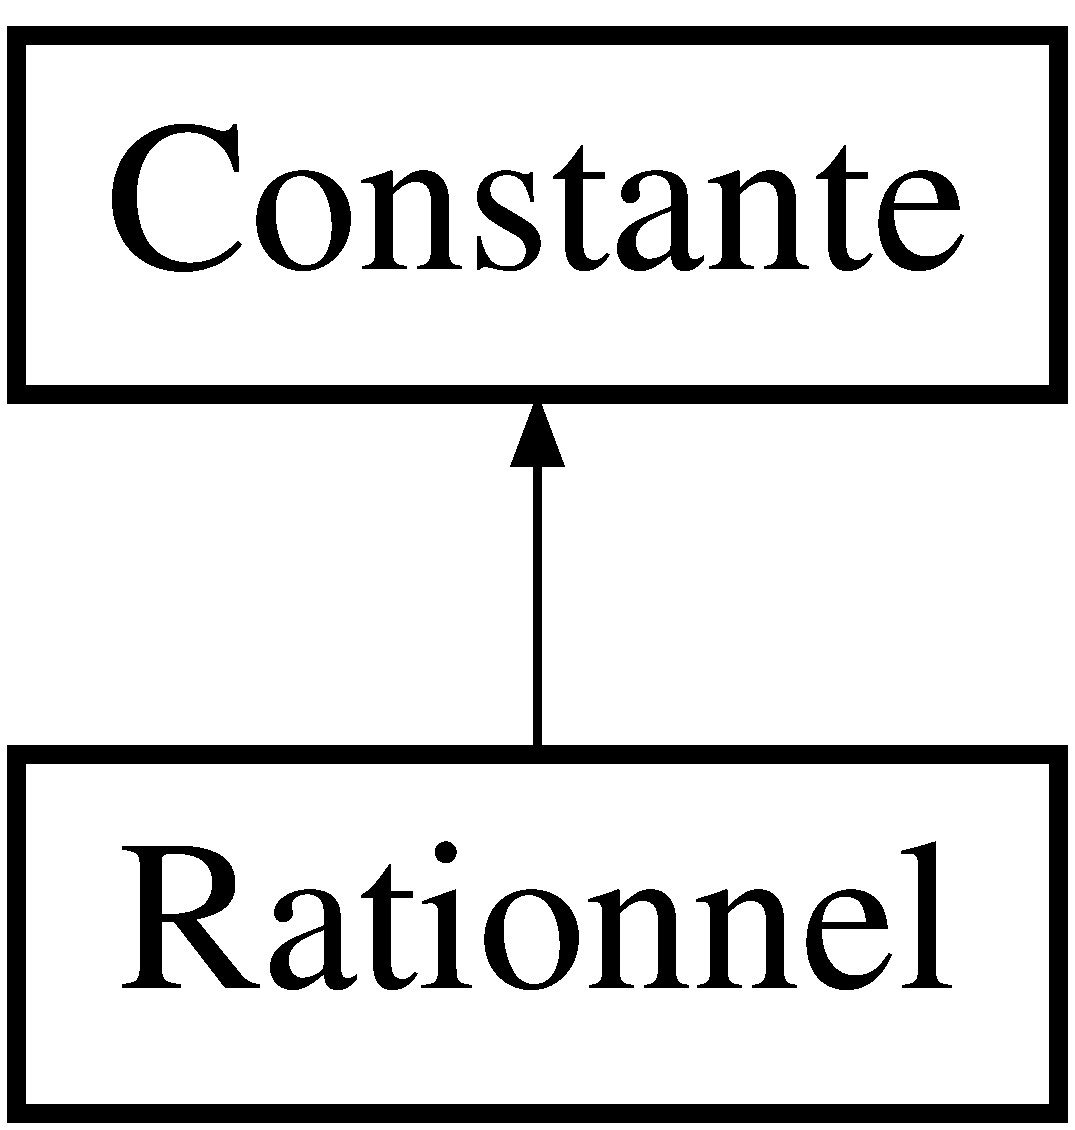
\includegraphics[height=2.000000cm]{class_rationnel}
\end{center}
\end{figure}
\subsection*{Public Member Functions}
\begin{DoxyCompactItemize}
\item 
\hyperlink{class_rationnel_aba6c7ac638004b5d553ee1d62c2c111f}{Rationnel} (const std\-::string \&)
\begin{DoxyCompactList}\small\item\em Constructeur Constructeur de la classe \hyperlink{class_rationnel}{Rationnel} initialisant le build\-Constante et le genre du rationnel. \end{DoxyCompactList}\item 
\hyperlink{class_rationnel_a089d09fa5fa91ae0a5ad825e736c3fba}{Rationnel} (const std\-::string \&val, const \hyperlink{constante_8h_a1d1cfd8ffb84e947f82999c682b666a7}{Type} \&T1, const \hyperlink{constante_8h_a1d1cfd8ffb84e947f82999c682b666a7}{Type} \&T2=\hyperlink{constante_8h_a1d1cfd8ffb84e947f82999c682b666a7a310a841612cf153caf2103c7d7136070}{entier})
\begin{DoxyCompactList}\small\item\em Constructeur Constructeur de la classe \hyperlink{class_rationnel}{Rationnel}. \end{DoxyCompactList}\item 
\hypertarget{class_rationnel_ab8eedc9cb8ea828e3e3d590da59ded6b}{\hyperlink{class_rationnel_ab8eedc9cb8ea828e3e3d590da59ded6b}{Rationnel} (const \hyperlink{class_rationnel}{Rationnel} \&)}\label{class_rationnel_ab8eedc9cb8ea828e3e3d590da59ded6b}

\begin{DoxyCompactList}\small\item\em Constructeur de recopie. \end{DoxyCompactList}\item 
int \hyperlink{class_rationnel_aae37d3512b67bcd6c5e52d64eb415738}{get\-Num\-\_\-int} () const 
\begin{DoxyCompactList}\small\item\em Accesseur. \end{DoxyCompactList}\item 
int \hyperlink{class_rationnel_afb7b64f485a337e4a3ab5b6c320cc919}{get\-Den\-\_\-int} () const 
\begin{DoxyCompactList}\small\item\em Accesseur. \end{DoxyCompactList}\item 
void \hyperlink{class_rationnel_ac0d040e03d9ba78582e8452038a76030}{set\-Num} (\hyperlink{class_entier}{Entier} $\ast$a)
\begin{DoxyCompactList}\small\item\em Accesseur. \end{DoxyCompactList}\item 
void \hyperlink{class_rationnel_aad905931a5bbcbd2a7487510c0be3e6a}{set\-Den} (\hyperlink{class_entier}{Entier} $\ast$a)
\begin{DoxyCompactList}\small\item\em Accesseur. \end{DoxyCompactList}\item 
\hyperlink{class_entier}{Entier} $\ast$ \hyperlink{class_rationnel_aa10a19c5b030dd007e7e071d6c4b5a75}{get\-Num} () const 
\begin{DoxyCompactList}\small\item\em Accesseur. \end{DoxyCompactList}\item 
\hyperlink{class_entier}{Entier} $\ast$ \hyperlink{class_rationnel_a77d9d3cb78f49260f92b981ab716b9fd}{get\-Den} () const 
\begin{DoxyCompactList}\small\item\em Accesseur. \end{DoxyCompactList}\item 
\hypertarget{class_rationnel_ab0257aa2fd1b258506ec6d2a268612c6}{\hyperlink{class_rationnel_ab0257aa2fd1b258506ec6d2a268612c6}{$\sim$\-Rationnel} ()}\label{class_rationnel_ab0257aa2fd1b258506ec6d2a268612c6}

\begin{DoxyCompactList}\small\item\em Destructeur Lib�re les pointeurs d'\hyperlink{class_entier}{Entier}. \end{DoxyCompactList}\item 
virtual std\-::string \hyperlink{class_rationnel_ad9911305f668f4f537d541bb82e60a6b}{get\-Chain} () const 
\begin{DoxyCompactList}\small\item\em Convertit en chaine le \hyperlink{class_rationnel}{Rationnel}. \end{DoxyCompactList}\item 
\hypertarget{class_rationnel_a10ba897af046ecefa02d0832fdcdcdbd}{\hyperlink{class_rationnel}{Rationnel} \& \hyperlink{class_rationnel_a10ba897af046ecefa02d0832fdcdcdbd}{operator+=} (\hyperlink{class_rationnel}{Rationnel} const \&e)}\label{class_rationnel_a10ba897af046ecefa02d0832fdcdcdbd}

\begin{DoxyCompactList}\small\item\em Surcharge de l'op�rateur +=. \end{DoxyCompactList}\item 
\hypertarget{class_rationnel_a4317efffac04faa9c79bc316a9902f68}{\hyperlink{class_rationnel}{Rationnel} \& \hyperlink{class_rationnel_a4317efffac04faa9c79bc316a9902f68}{operator-\/=} (\hyperlink{class_rationnel}{Rationnel} const \&e)}\label{class_rationnel_a4317efffac04faa9c79bc316a9902f68}

\begin{DoxyCompactList}\small\item\em Surcharge de l'op�rateur -\/=. \end{DoxyCompactList}\item 
\hypertarget{class_rationnel_a73bc375174c0ce7478755c22f4a2d972}{\hyperlink{class_rationnel}{Rationnel} \& \hyperlink{class_rationnel_a73bc375174c0ce7478755c22f4a2d972}{operator$\ast$=} (\hyperlink{class_rationnel}{Rationnel} const \&e)}\label{class_rationnel_a73bc375174c0ce7478755c22f4a2d972}

\begin{DoxyCompactList}\small\item\em Surcharge de l'op�rateur $\ast$=. \end{DoxyCompactList}\item 
\hypertarget{class_rationnel_a836c26b6b1c18e967954ade01e3c93a4}{\hyperlink{class_rationnel}{Rationnel} \& \hyperlink{class_rationnel_a836c26b6b1c18e967954ade01e3c93a4}{operator/=} (\hyperlink{class_rationnel}{Rationnel} const \&e)}\label{class_rationnel_a836c26b6b1c18e967954ade01e3c93a4}

\begin{DoxyCompactList}\small\item\em Surcharge de l'op�rateur /=. \end{DoxyCompactList}\item 
\hypertarget{class_rationnel_a12ee060e5fca5f4291b222983d727268}{void \hyperlink{class_rationnel_a12ee060e5fca5f4291b222983d727268}{simplifier} ()}\label{class_rationnel_a12ee060e5fca5f4291b222983d727268}

\begin{DoxyCompactList}\small\item\em Simplifie le \hyperlink{class_rationnel}{Rationnel}. \end{DoxyCompactList}\end{DoxyCompactItemize}
\subsection*{Private Member Functions}
\begin{DoxyCompactItemize}
\item 
virtual void \hyperlink{class_rationnel_a3ee911afa5c5411814ab36b8cac948d7}{build\-Constant} (const std\-::string \&)
\end{DoxyCompactItemize}
\subsection*{Private Attributes}
\begin{DoxyCompactItemize}
\item 
\hyperlink{class_entier}{Entier} $\ast$ \hyperlink{class_rationnel_a87d71d6aa449da998ff5352995058952}{numerateur}
\item 
\hyperlink{class_entier}{Entier} $\ast$ \hyperlink{class_rationnel_ac161bfd8308b1e3042178f81865a05e8}{denominateur}
\end{DoxyCompactItemize}


\subsection{Constructor \& Destructor Documentation}
\hypertarget{class_rationnel_aba6c7ac638004b5d553ee1d62c2c111f}{\index{Rationnel@{Rationnel}!Rationnel@{Rationnel}}
\index{Rationnel@{Rationnel}!Rationnel@{Rationnel}}
\subsubsection[{Rationnel}]{\setlength{\rightskip}{0pt plus 5cm}{\bf Rationnel\-::\-Rationnel} (
\begin{DoxyParamCaption}
\item[{const std\-::string \&}]{val}
\end{DoxyParamCaption}
)}}\label{class_rationnel_aba6c7ac638004b5d553ee1d62c2c111f}


Constructeur Constructeur de la classe \hyperlink{class_rationnel}{Rationnel} initialisant le build\-Constante et le genre du rationnel. 


\begin{DoxyParams}{Parameters}
{\em string} & \-: build\-Constante \\
\hline
\end{DoxyParams}
\hypertarget{class_rationnel_a089d09fa5fa91ae0a5ad825e736c3fba}{\index{Rationnel@{Rationnel}!Rationnel@{Rationnel}}
\index{Rationnel@{Rationnel}!Rationnel@{Rationnel}}
\subsubsection[{Rationnel}]{\setlength{\rightskip}{0pt plus 5cm}{\bf Rationnel\-::\-Rationnel} (
\begin{DoxyParamCaption}
\item[{const std\-::string \&}]{val, }
\item[{const {\bf Type} \&}]{T1, }
\item[{const {\bf Type} \&}]{T2 = {\ttfamily {\bf entier}}}
\end{DoxyParamCaption}
)}}\label{class_rationnel_a089d09fa5fa91ae0a5ad825e736c3fba}


Constructeur Constructeur de la classe \hyperlink{class_rationnel}{Rationnel}. 


\begin{DoxyParams}{Parameters}
{\em val} & \-: string \\
\hline
{\em T1} & \-: Type de la constante contenue dans val \\
\hline
{\em T2} & \-: Type du contenu du complexe que l'on peut transmettre si on le souhaite \\
\hline
\end{DoxyParams}


\subsection{Member Function Documentation}
\hypertarget{class_rationnel_a3ee911afa5c5411814ab36b8cac948d7}{\index{Rationnel@{Rationnel}!build\-Constant@{build\-Constant}}
\index{build\-Constant@{build\-Constant}!Rationnel@{Rationnel}}
\subsubsection[{build\-Constant}]{\setlength{\rightskip}{0pt plus 5cm}void {\bf Rationnel\-::build\-Constant} (
\begin{DoxyParamCaption}
\item[{const std\-::string \&}]{val}
\end{DoxyParamCaption}
)\hspace{0.3cm}{\ttfamily  \mbox{[}private, virtual\mbox{]}}}}\label{class_rationnel_a3ee911afa5c5411814ab36b8cac948d7}
Construit la \hyperlink{class_constante}{Constante} empilable 

Implements \hyperlink{class_constante_afc5d0bb9363678d5b37543b5394c571e}{Constante}.

\hypertarget{class_rationnel_ad9911305f668f4f537d541bb82e60a6b}{\index{Rationnel@{Rationnel}!get\-Chain@{get\-Chain}}
\index{get\-Chain@{get\-Chain}!Rationnel@{Rationnel}}
\subsubsection[{get\-Chain}]{\setlength{\rightskip}{0pt plus 5cm}std\-::string {\bf Rationnel\-::get\-Chain} (
\begin{DoxyParamCaption}
{}
\end{DoxyParamCaption}
) const\hspace{0.3cm}{\ttfamily  \mbox{[}virtual\mbox{]}}}}\label{class_rationnel_ad9911305f668f4f537d541bb82e60a6b}


Convertit en chaine le \hyperlink{class_rationnel}{Rationnel}. 

\begin{DoxyReturn}{Returns}
La chaine correspondante au \hyperlink{class_rationnel}{Rationnel} 
\end{DoxyReturn}


Implements \hyperlink{class_constante_abd8a7f18b934053173ab87d947bd3386}{Constante}.

\hypertarget{class_rationnel_a77d9d3cb78f49260f92b981ab716b9fd}{\index{Rationnel@{Rationnel}!get\-Den@{get\-Den}}
\index{get\-Den@{get\-Den}!Rationnel@{Rationnel}}
\subsubsection[{get\-Den}]{\setlength{\rightskip}{0pt plus 5cm}{\bf Entier}$\ast$ {\bf Rationnel\-::get\-Den} (
\begin{DoxyParamCaption}
{}
\end{DoxyParamCaption}
) const\hspace{0.3cm}{\ttfamily  \mbox{[}inline\mbox{]}}}}\label{class_rationnel_a77d9d3cb78f49260f92b981ab716b9fd}


Accesseur. 

\begin{DoxyReturn}{Returns}
Le d�nominateur entant qu'\hyperlink{class_entier}{Entier} 
\end{DoxyReturn}
\hypertarget{class_rationnel_afb7b64f485a337e4a3ab5b6c320cc919}{\index{Rationnel@{Rationnel}!get\-Den\-\_\-int@{get\-Den\-\_\-int}}
\index{get\-Den\-\_\-int@{get\-Den\-\_\-int}!Rationnel@{Rationnel}}
\subsubsection[{get\-Den\-\_\-int}]{\setlength{\rightskip}{0pt plus 5cm}int {\bf Rationnel\-::get\-Den\-\_\-int} (
\begin{DoxyParamCaption}
{}
\end{DoxyParamCaption}
) const\hspace{0.3cm}{\ttfamily  \mbox{[}inline\mbox{]}}}}\label{class_rationnel_afb7b64f485a337e4a3ab5b6c320cc919}


Accesseur. 

\begin{DoxyReturn}{Returns}
Le d�nominateur entant qu' int 
\end{DoxyReturn}
\hypertarget{class_rationnel_aa10a19c5b030dd007e7e071d6c4b5a75}{\index{Rationnel@{Rationnel}!get\-Num@{get\-Num}}
\index{get\-Num@{get\-Num}!Rationnel@{Rationnel}}
\subsubsection[{get\-Num}]{\setlength{\rightskip}{0pt plus 5cm}{\bf Entier}$\ast$ {\bf Rationnel\-::get\-Num} (
\begin{DoxyParamCaption}
{}
\end{DoxyParamCaption}
) const\hspace{0.3cm}{\ttfamily  \mbox{[}inline\mbox{]}}}}\label{class_rationnel_aa10a19c5b030dd007e7e071d6c4b5a75}


Accesseur. 

\begin{DoxyReturn}{Returns}
Le num�rateur entant qu'\hyperlink{class_entier}{Entier} 
\end{DoxyReturn}
\hypertarget{class_rationnel_aae37d3512b67bcd6c5e52d64eb415738}{\index{Rationnel@{Rationnel}!get\-Num\-\_\-int@{get\-Num\-\_\-int}}
\index{get\-Num\-\_\-int@{get\-Num\-\_\-int}!Rationnel@{Rationnel}}
\subsubsection[{get\-Num\-\_\-int}]{\setlength{\rightskip}{0pt plus 5cm}int {\bf Rationnel\-::get\-Num\-\_\-int} (
\begin{DoxyParamCaption}
{}
\end{DoxyParamCaption}
) const\hspace{0.3cm}{\ttfamily  \mbox{[}inline\mbox{]}}}}\label{class_rationnel_aae37d3512b67bcd6c5e52d64eb415738}


Accesseur. 

\begin{DoxyReturn}{Returns}
Le num�rateur entant qu' int 
\end{DoxyReturn}
\hypertarget{class_rationnel_aad905931a5bbcbd2a7487510c0be3e6a}{\index{Rationnel@{Rationnel}!set\-Den@{set\-Den}}
\index{set\-Den@{set\-Den}!Rationnel@{Rationnel}}
\subsubsection[{set\-Den}]{\setlength{\rightskip}{0pt plus 5cm}void {\bf Rationnel\-::set\-Den} (
\begin{DoxyParamCaption}
\item[{{\bf Entier} $\ast$}]{a}
\end{DoxyParamCaption}
)\hspace{0.3cm}{\ttfamily  \mbox{[}inline\mbox{]}}}}\label{class_rationnel_aad905931a5bbcbd2a7487510c0be3e6a}


Accesseur. 

\begin{DoxyReturn}{Returns}
Change la valeur du d�nominateur 
\end{DoxyReturn}
\hypertarget{class_rationnel_ac0d040e03d9ba78582e8452038a76030}{\index{Rationnel@{Rationnel}!set\-Num@{set\-Num}}
\index{set\-Num@{set\-Num}!Rationnel@{Rationnel}}
\subsubsection[{set\-Num}]{\setlength{\rightskip}{0pt plus 5cm}void {\bf Rationnel\-::set\-Num} (
\begin{DoxyParamCaption}
\item[{{\bf Entier} $\ast$}]{a}
\end{DoxyParamCaption}
)\hspace{0.3cm}{\ttfamily  \mbox{[}inline\mbox{]}}}}\label{class_rationnel_ac0d040e03d9ba78582e8452038a76030}


Accesseur. 

\begin{DoxyReturn}{Returns}
Change la valeur du num�rateur 
\end{DoxyReturn}


\subsection{Member Data Documentation}
\hypertarget{class_rationnel_ac161bfd8308b1e3042178f81865a05e8}{\index{Rationnel@{Rationnel}!denominateur@{denominateur}}
\index{denominateur@{denominateur}!Rationnel@{Rationnel}}
\subsubsection[{denominateur}]{\setlength{\rightskip}{0pt plus 5cm}{\bf Entier}$\ast$ {\bf Rationnel\-::denominateur}\hspace{0.3cm}{\ttfamily  \mbox{[}private\mbox{]}}}}\label{class_rationnel_ac161bfd8308b1e3042178f81865a05e8}
d�nominateur \hypertarget{class_rationnel_a87d71d6aa449da998ff5352995058952}{\index{Rationnel@{Rationnel}!numerateur@{numerateur}}
\index{numerateur@{numerateur}!Rationnel@{Rationnel}}
\subsubsection[{numerateur}]{\setlength{\rightskip}{0pt plus 5cm}{\bf Entier}$\ast$ {\bf Rationnel\-::numerateur}\hspace{0.3cm}{\ttfamily  \mbox{[}private\mbox{]}}}}\label{class_rationnel_a87d71d6aa449da998ff5352995058952}
num�rateur 

The documentation for this class was generated from the following files\-:\begin{DoxyCompactItemize}
\item 
rationnel.\-h\item 
rationnel.\-cpp\end{DoxyCompactItemize}

\hypertarget{class_reel}{\section{Reel Class Reference}
\label{class_reel}\index{Reel@{Reel}}
}


classe definissant le type \hyperlink{class_reel}{Reel} herite de la classe \hyperlink{class_constante}{Constante}  




{\ttfamily \#include $<$reel.\-h$>$}

Inheritance diagram for Reel\-:\begin{figure}[H]
\begin{center}
\leavevmode
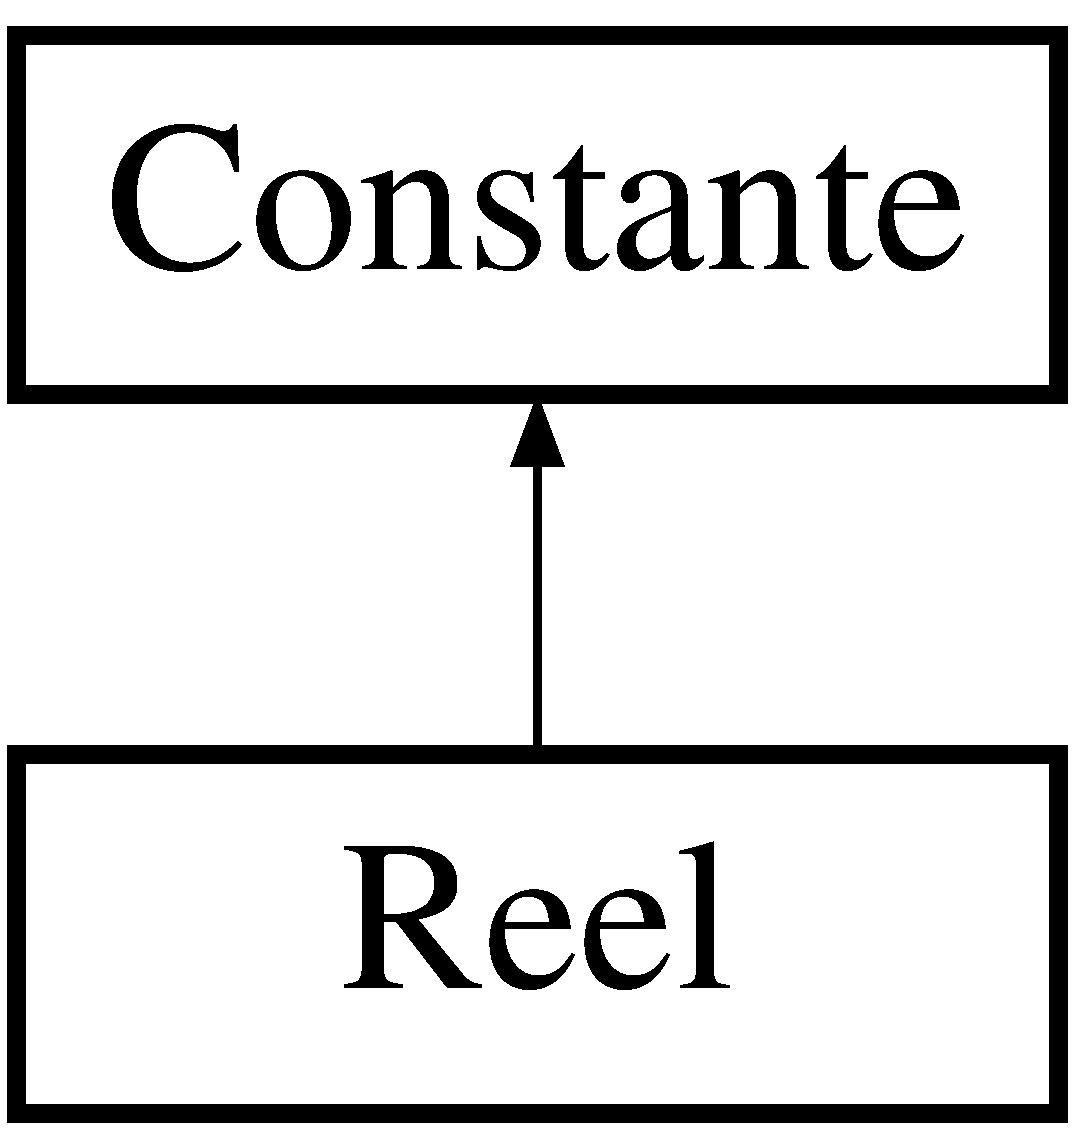
\includegraphics[height=2.000000cm]{class_reel}
\end{center}
\end{figure}
\subsection*{Public Member Functions}
\begin{DoxyCompactItemize}
\item 
\hyperlink{class_reel_ad872399c3ce40c9ff5cbda4d55b95f53}{Reel} (const std\-::string \&val)
\begin{DoxyCompactList}\small\item\em Constructeur Constructeur de la classe \hyperlink{class_reel}{Reel}. \end{DoxyCompactList}\item 
\hyperlink{class_reel_a6e9e3b9984388324fa8d4798adaeec4e}{Reel} (const std\-::string \&val, const \hyperlink{constante_8h_a1d1cfd8ffb84e947f82999c682b666a7}{Type} \&T1, const \hyperlink{constante_8h_a1d1cfd8ffb84e947f82999c682b666a7}{Type} \&T2=\hyperlink{constante_8h_a1d1cfd8ffb84e947f82999c682b666a7a310a841612cf153caf2103c7d7136070}{entier})
\begin{DoxyCompactList}\small\item\em Constructeur Constructeur de la classe \hyperlink{class_reel}{Reel}. \end{DoxyCompactList}\item 
float \hyperlink{class_reel_a66d6f1cfe4fa7665f7f83e242a816a5a}{get\-Val} () const 
\begin{DoxyCompactList}\small\item\em Accesseur. \end{DoxyCompactList}\item 
void \hyperlink{class_reel_a3ed5bc535aeaee9ffb4bbc63a5db58e0}{set\-Val} (float f)
\begin{DoxyCompactList}\small\item\em Accesseur. \end{DoxyCompactList}\item 
virtual std\-::string \hyperlink{class_reel_aef757f3ab4b4fcea2b788fcafb10e8d1}{get\-Chain} () const 
\begin{DoxyCompactList}\small\item\em Convertisseur. \end{DoxyCompactList}\item 
\hypertarget{class_reel_a1a4fbbbf7303084e06b76cf2cfdeede4}{\hyperlink{class_reel}{Reel} \& \hyperlink{class_reel_a1a4fbbbf7303084e06b76cf2cfdeede4}{operator+=} (\hyperlink{class_reel}{Reel} const \&e)}\label{class_reel_a1a4fbbbf7303084e06b76cf2cfdeede4}

\begin{DoxyCompactList}\small\item\em Surcharge de +=. \end{DoxyCompactList}\item 
\hypertarget{class_reel_a33890251396e0c9d0e1147aaf537b388}{\hyperlink{class_reel}{Reel} \& \hyperlink{class_reel_a33890251396e0c9d0e1147aaf537b388}{operator-\/=} (\hyperlink{class_reel}{Reel} const \&e)}\label{class_reel_a33890251396e0c9d0e1147aaf537b388}

\begin{DoxyCompactList}\small\item\em Surcharge de -\/=. \end{DoxyCompactList}\item 
\hypertarget{class_reel_a36af4a7c4d941eafbe0f4000aaa51c37}{\hyperlink{class_reel}{Reel} \& \hyperlink{class_reel_a36af4a7c4d941eafbe0f4000aaa51c37}{operator$\ast$=} (\hyperlink{class_reel}{Reel} const \&e)}\label{class_reel_a36af4a7c4d941eafbe0f4000aaa51c37}

\begin{DoxyCompactList}\small\item\em Surcharge de $\ast$=. \end{DoxyCompactList}\item 
\hypertarget{class_reel_ad6a9191c56939de0c4d02296f7cb74fc}{\hyperlink{class_reel}{Reel} \& \hyperlink{class_reel_ad6a9191c56939de0c4d02296f7cb74fc}{operator/=} (\hyperlink{class_reel}{Reel} const \&e)}\label{class_reel_ad6a9191c56939de0c4d02296f7cb74fc}

\begin{DoxyCompactList}\small\item\em Surcharge de /=. \end{DoxyCompactList}\end{DoxyCompactItemize}
\subsection*{Private Member Functions}
\begin{DoxyCompactItemize}
\item 
virtual void \hyperlink{class_reel_a4b36b8926b60feedeb391dcdb7bb2e6e}{build\-Constant} (const std\-::string \&)
\end{DoxyCompactItemize}
\subsection*{Private Attributes}
\begin{DoxyCompactItemize}
\item 
float \hyperlink{class_reel_a9404b0067ebe02f9a6cfffb1094c0cc7}{valeur}
\end{DoxyCompactItemize}


\subsection{Detailed Description}
classe definissant le type \hyperlink{class_reel}{Reel} herite de la classe \hyperlink{class_constante}{Constante} 

\subsection{Constructor \& Destructor Documentation}
\hypertarget{class_reel_ad872399c3ce40c9ff5cbda4d55b95f53}{\index{Reel@{Reel}!Reel@{Reel}}
\index{Reel@{Reel}!Reel@{Reel}}
\subsubsection[{Reel}]{\setlength{\rightskip}{0pt plus 5cm}{\bf Reel\-::\-Reel} (
\begin{DoxyParamCaption}
\item[{const std\-::string \&}]{val}
\end{DoxyParamCaption}
)}}\label{class_reel_ad872399c3ce40c9ff5cbda4d55b95f53}


Constructeur Constructeur de la classe \hyperlink{class_reel}{Reel}. 


\begin{DoxyParams}{Parameters}
{\em val} & \-: string \\
\hline
\end{DoxyParams}
\hypertarget{class_reel_a6e9e3b9984388324fa8d4798adaeec4e}{\index{Reel@{Reel}!Reel@{Reel}}
\index{Reel@{Reel}!Reel@{Reel}}
\subsubsection[{Reel}]{\setlength{\rightskip}{0pt plus 5cm}{\bf Reel\-::\-Reel} (
\begin{DoxyParamCaption}
\item[{const std\-::string \&}]{val, }
\item[{const {\bf Type} \&}]{T1, }
\item[{const {\bf Type} \&}]{T2 = {\ttfamily {\bf entier}}}
\end{DoxyParamCaption}
)}}\label{class_reel_a6e9e3b9984388324fa8d4798adaeec4e}


Constructeur Constructeur de la classe \hyperlink{class_reel}{Reel}. 


\begin{DoxyParams}{Parameters}
{\em val} & \-: string \\
\hline
{\em T1} & \-: Type de la constante contenue dans val \\
\hline
{\em T2} & \-: Type du contenu du complexe que l'on peut transmettre si on le souhaite \\
\hline
\end{DoxyParams}


\subsection{Member Function Documentation}
\hypertarget{class_reel_a4b36b8926b60feedeb391dcdb7bb2e6e}{\index{Reel@{Reel}!build\-Constant@{build\-Constant}}
\index{build\-Constant@{build\-Constant}!Reel@{Reel}}
\subsubsection[{build\-Constant}]{\setlength{\rightskip}{0pt plus 5cm}void {\bf Reel\-::build\-Constant} (
\begin{DoxyParamCaption}
\item[{const std\-::string \&}]{val}
\end{DoxyParamCaption}
)\hspace{0.3cm}{\ttfamily  \mbox{[}private, virtual\mbox{]}}}}\label{class_reel_a4b36b8926b60feedeb391dcdb7bb2e6e}
Constructeur de \hyperlink{class_constante}{Constante} empilable 

Implements \hyperlink{class_constante_afc5d0bb9363678d5b37543b5394c571e}{Constante}.

\hypertarget{class_reel_aef757f3ab4b4fcea2b788fcafb10e8d1}{\index{Reel@{Reel}!get\-Chain@{get\-Chain}}
\index{get\-Chain@{get\-Chain}!Reel@{Reel}}
\subsubsection[{get\-Chain}]{\setlength{\rightskip}{0pt plus 5cm}std\-::string {\bf Reel\-::get\-Chain} (
\begin{DoxyParamCaption}
{}
\end{DoxyParamCaption}
) const\hspace{0.3cm}{\ttfamily  \mbox{[}virtual\mbox{]}}}}\label{class_reel_aef757f3ab4b4fcea2b788fcafb10e8d1}


Convertisseur. 

\begin{DoxyReturn}{Returns}
Une chaine correspondant � la valeur du reel 
\end{DoxyReturn}


Implements \hyperlink{class_constante_abd8a7f18b934053173ab87d947bd3386}{Constante}.

\hypertarget{class_reel_a66d6f1cfe4fa7665f7f83e242a816a5a}{\index{Reel@{Reel}!get\-Val@{get\-Val}}
\index{get\-Val@{get\-Val}!Reel@{Reel}}
\subsubsection[{get\-Val}]{\setlength{\rightskip}{0pt plus 5cm}float {\bf Reel\-::get\-Val} (
\begin{DoxyParamCaption}
{}
\end{DoxyParamCaption}
) const\hspace{0.3cm}{\ttfamily  \mbox{[}inline\mbox{]}}}}\label{class_reel_a66d6f1cfe4fa7665f7f83e242a816a5a}


Accesseur. 

\begin{DoxyReturn}{Returns}
Valeur du reel 
\end{DoxyReturn}
\hypertarget{class_reel_a3ed5bc535aeaee9ffb4bbc63a5db58e0}{\index{Reel@{Reel}!set\-Val@{set\-Val}}
\index{set\-Val@{set\-Val}!Reel@{Reel}}
\subsubsection[{set\-Val}]{\setlength{\rightskip}{0pt plus 5cm}void {\bf Reel\-::set\-Val} (
\begin{DoxyParamCaption}
\item[{float}]{f}
\end{DoxyParamCaption}
)\hspace{0.3cm}{\ttfamily  \mbox{[}inline\mbox{]}}}}\label{class_reel_a3ed5bc535aeaee9ffb4bbc63a5db58e0}


Accesseur. 

\begin{DoxyReturn}{Returns}
Modifie la valeur du reel 
\end{DoxyReturn}


\subsection{Member Data Documentation}
\hypertarget{class_reel_a9404b0067ebe02f9a6cfffb1094c0cc7}{\index{Reel@{Reel}!valeur@{valeur}}
\index{valeur@{valeur}!Reel@{Reel}}
\subsubsection[{valeur}]{\setlength{\rightskip}{0pt plus 5cm}float {\bf Reel\-::valeur}\hspace{0.3cm}{\ttfamily  \mbox{[}private\mbox{]}}}}\label{class_reel_a9404b0067ebe02f9a6cfffb1094c0cc7}
Valeur du reel 

The documentation for this class was generated from the following files\-:\begin{DoxyCompactItemize}
\item 
\hyperlink{reel_8h}{reel.\-h}\item 
reel.\-cpp\end{DoxyCompactItemize}

\hypertarget{class_swap_pile}{\section{Swap\-Pile Class Reference}
\label{class_swap_pile}\index{Swap\-Pile@{Swap\-Pile}}
}


Classe pour la gestion des echanges sur la pile.  




{\ttfamily \#include $<$mainwindow.\-h$>$}

\subsection*{Public Member Functions}
\begin{DoxyCompactItemize}
\item 
\hypertarget{class_swap_pile_a0c1c16257fc1c79db334a0bf4dd1fcbc}{\hyperlink{class_swap_pile_a0c1c16257fc1c79db334a0bf4dd1fcbc}{Swap\-Pile} (int i, int j, Q\-Undo\-Command $\ast$parent=0)}\label{class_swap_pile_a0c1c16257fc1c79db334a0bf4dd1fcbc}

\begin{DoxyCompactList}\small\item\em Constructeur de \hyperlink{class_swap_pile}{Swap\-Pile}. \end{DoxyCompactList}\item 
\hypertarget{class_swap_pile_a6aa712758cebcb7a525b569a3ed89029}{void \hyperlink{class_swap_pile_a6aa712758cebcb7a525b569a3ed89029}{undo} ()}\label{class_swap_pile_a6aa712758cebcb7a525b569a3ed89029}

\begin{DoxyCompactList}\small\item\em Change de place deux constantes choisies action identique � la fonction \hyperlink{class_swap_pile}{Swap\-Pile}. \end{DoxyCompactList}\item 
\hypertarget{class_swap_pile_a2e212405f9bd6d5e7d9710394efddf6d}{void \hyperlink{class_swap_pile_a2e212405f9bd6d5e7d9710394efddf6d}{redo} ()}\label{class_swap_pile_a2e212405f9bd6d5e7d9710394efddf6d}

\begin{DoxyCompactList}\small\item\em Change de place deux constantes choisies action identique � la fonction \hyperlink{class_swap_pile}{Swap\-Pile}. \end{DoxyCompactList}\end{DoxyCompactItemize}
\subsection*{Private Attributes}
\begin{DoxyCompactItemize}
\item 
\hypertarget{class_swap_pile_a97720bda698690d803bb923747a68918}{int {\bfseries f}}\label{class_swap_pile_a97720bda698690d803bb923747a68918}

\item 
int \hyperlink{class_swap_pile_a6047f2f2433d7ee39a102b83540688cb}{l}
\end{DoxyCompactItemize}


\subsection{Detailed Description}
Classe pour la gestion des echanges sur la pile. 

\subsection{Member Data Documentation}
\hypertarget{class_swap_pile_a6047f2f2433d7ee39a102b83540688cb}{\index{Swap\-Pile@{Swap\-Pile}!l@{l}}
\index{l@{l}!SwapPile@{Swap\-Pile}}
\subsubsection[{l}]{\setlength{\rightskip}{0pt plus 5cm}int {\bf Swap\-Pile\-::l}\hspace{0.3cm}{\ttfamily  \mbox{[}private\mbox{]}}}}\label{class_swap_pile_a6047f2f2433d7ee39a102b83540688cb}
places dans la pile des constantes � �changer 

The documentation for this class was generated from the following files\-:\begin{DoxyCompactItemize}
\item 
\hyperlink{mainwindow_8h}{mainwindow.\-h}\item 
mainwindow.\-cpp\end{DoxyCompactItemize}

\chapter{File Documentation}
\hypertarget{complexe_8h}{\section{complexe.\-h File Reference}
\label{complexe_8h}\index{complexe.\-h@{complexe.\-h}}
}


classe complexe et toutes les fonctions associ�es  


{\ttfamily \#include \char`\"{}constante.\-h\char`\"{}}\\*
{\ttfamily \#include \char`\"{}entier.\-h\char`\"{}}\\*
{\ttfamily \#include \char`\"{}rationnel.\-h\char`\"{}}\\*
{\ttfamily \#include \char`\"{}reel.\-h\char`\"{}}\\*
\subsection*{Classes}
\begin{DoxyCompactItemize}
\item 
class \hyperlink{class_complexe}{Complexe}
\begin{DoxyCompactList}\small\item\em classe definissant le type \hyperlink{class_complexe}{Complexe} herite de la classe \hyperlink{class_constante}{Constante} \end{DoxyCompactList}\end{DoxyCompactItemize}
\subsection*{Functions}
\begin{DoxyCompactItemize}
\item 
\hypertarget{complexe_8h_a1bc94f522fb9a167100cad9cfe718047}{\hyperlink{class_complexe}{Complexe} \hyperlink{complexe_8h_a1bc94f522fb9a167100cad9cfe718047}{operator+} (\hyperlink{class_complexe}{Complexe} const \&a, \hyperlink{class_complexe}{Complexe} const \&b)}\label{complexe_8h_a1bc94f522fb9a167100cad9cfe718047}

\begin{DoxyCompactList}\small\item\em Surcharge de +. \end{DoxyCompactList}\item 
\hypertarget{complexe_8h_a500853af687505966075574c2b3d9dac}{\hyperlink{class_complexe}{Complexe} \hyperlink{complexe_8h_a500853af687505966075574c2b3d9dac}{operator-\/} (\hyperlink{class_complexe}{Complexe} const \&a, \hyperlink{class_complexe}{Complexe} const \&b)}\label{complexe_8h_a500853af687505966075574c2b3d9dac}

\begin{DoxyCompactList}\small\item\em Surcharge de -\/. \end{DoxyCompactList}\item 
\hypertarget{complexe_8h_a02034dc26d95f660952ca465449cebc8}{\hyperlink{class_complexe}{Complexe} \hyperlink{complexe_8h_a02034dc26d95f660952ca465449cebc8}{operator$\ast$} (\hyperlink{class_complexe}{Complexe} const \&a, \hyperlink{class_complexe}{Complexe} const \&b)}\label{complexe_8h_a02034dc26d95f660952ca465449cebc8}

\begin{DoxyCompactList}\small\item\em Surcharge de $\ast$. \end{DoxyCompactList}\item 
\hypertarget{complexe_8h_a9bd1f8ef5f6f90e0ced8853ea055c768}{\hyperlink{class_complexe}{Complexe} \hyperlink{complexe_8h_a9bd1f8ef5f6f90e0ced8853ea055c768}{operator/} (\hyperlink{class_complexe}{Complexe} const \&a, \hyperlink{class_complexe}{Complexe} const \&b)}\label{complexe_8h_a9bd1f8ef5f6f90e0ced8853ea055c768}

\begin{DoxyCompactList}\small\item\em Surcharge de /. \end{DoxyCompactList}\end{DoxyCompactItemize}


\subsection{Detailed Description}
classe complexe et toutes les fonctions associ�es \begin{DoxyAuthor}{Author}
Frederic Roge, Paul Villain 
\end{DoxyAuthor}

\hypertarget{constante_8h}{\section{constante.\-h File Reference}
\label{constante_8h}\index{constante.\-h@{constante.\-h}}
}


classe constante et toutes les fonctions associ�es  


{\ttfamily \#include $<$iostream$>$}\\*
{\ttfamily \#include $<$string$>$}\\*
{\ttfamily \#include $<$cstdlib$>$}\\*
{\ttfamily \#include $<$sstream$>$}\\*
\subsection*{Classes}
\begin{DoxyCompactItemize}
\item 
class \hyperlink{class_constante}{Constante}
\begin{DoxyCompactList}\small\item\em D�fini le type de \hyperlink{class_constante}{Constante}. \end{DoxyCompactList}\end{DoxyCompactItemize}
\subsection*{Enumerations}
\begin{DoxyCompactItemize}
\item 
enum \hyperlink{constante_8h_a1d1cfd8ffb84e947f82999c682b666a7}{Type} \{ \\*
\hyperlink{constante_8h_a1d1cfd8ffb84e947f82999c682b666a7a310a841612cf153caf2103c7d7136070}{entier}, 
\hyperlink{constante_8h_a1d1cfd8ffb84e947f82999c682b666a7a0ec75e38f86c720d5b37dac4e7efbeb5}{rationnel}, 
\hyperlink{constante_8h_a1d1cfd8ffb84e947f82999c682b666a7ab76fc0da4fc267a87fce3e239e9b0290}{reel}, 
\hyperlink{constante_8h_a1d1cfd8ffb84e947f82999c682b666a7ab5b3a46d90ce465f0ad4c9f7a51b1102}{complexe}, 
\\*
\hyperlink{constante_8h_a1d1cfd8ffb84e947f82999c682b666a7ac810bbb61792a076f46cad2c89d87e1d}{expression}, 
\hyperlink{constante_8h_a1d1cfd8ffb84e947f82999c682b666a7a6de88b3aa37df025614e5ddc99481546}{erreur}
 \}
\begin{DoxyCompactList}\small\item\em Enum�re les types de \hyperlink{class_constante}{Constante}. \end{DoxyCompactList}\end{DoxyCompactItemize}


\subsection{Detailed Description}
classe constante et toutes les fonctions associ�es \begin{DoxyAuthor}{Author}
Frederic Roge, Paul Villain 
\end{DoxyAuthor}


\subsection{Enumeration Type Documentation}
\hypertarget{constante_8h_a1d1cfd8ffb84e947f82999c682b666a7}{\index{constante.\-h@{constante.\-h}!Type@{Type}}
\index{Type@{Type}!constante.h@{constante.\-h}}
\subsubsection[{Type}]{\setlength{\rightskip}{0pt plus 5cm}enum {\bf Type}}}\label{constante_8h_a1d1cfd8ffb84e947f82999c682b666a7}


Enum�re les types de \hyperlink{class_constante}{Constante}. 

\begin{Desc}
\item[Enumerator\-: ]\par
\begin{description}
\index{entier@{entier}!constante.\-h@{constante.\-h}}\index{constante.\-h@{constante.\-h}!entier@{entier}}\item[{\em 
\hypertarget{constante_8h_a1d1cfd8ffb84e947f82999c682b666a7a310a841612cf153caf2103c7d7136070}{entier}\label{constante_8h_a1d1cfd8ffb84e947f82999c682b666a7a310a841612cf153caf2103c7d7136070}
}]Type entier \index{rationnel@{rationnel}!constante.\-h@{constante.\-h}}\index{constante.\-h@{constante.\-h}!rationnel@{rationnel}}\item[{\em 
\hypertarget{constante_8h_a1d1cfd8ffb84e947f82999c682b666a7a0ec75e38f86c720d5b37dac4e7efbeb5}{rationnel}\label{constante_8h_a1d1cfd8ffb84e947f82999c682b666a7a0ec75e38f86c720d5b37dac4e7efbeb5}
}]Type rationnel \index{reel@{reel}!constante.\-h@{constante.\-h}}\index{constante.\-h@{constante.\-h}!reel@{reel}}\item[{\em 
\hypertarget{constante_8h_a1d1cfd8ffb84e947f82999c682b666a7ab76fc0da4fc267a87fce3e239e9b0290}{reel}\label{constante_8h_a1d1cfd8ffb84e947f82999c682b666a7ab76fc0da4fc267a87fce3e239e9b0290}
}]Type reel \index{complexe@{complexe}!constante.\-h@{constante.\-h}}\index{constante.\-h@{constante.\-h}!complexe@{complexe}}\item[{\em 
\hypertarget{constante_8h_a1d1cfd8ffb84e947f82999c682b666a7ab5b3a46d90ce465f0ad4c9f7a51b1102}{complexe}\label{constante_8h_a1d1cfd8ffb84e947f82999c682b666a7ab5b3a46d90ce465f0ad4c9f7a51b1102}
}]Type complexe \index{expression@{expression}!constante.\-h@{constante.\-h}}\index{constante.\-h@{constante.\-h}!expression@{expression}}\item[{\em 
\hypertarget{constante_8h_a1d1cfd8ffb84e947f82999c682b666a7ac810bbb61792a076f46cad2c89d87e1d}{expression}\label{constante_8h_a1d1cfd8ffb84e947f82999c682b666a7ac810bbb61792a076f46cad2c89d87e1d}
}]Type expression \index{erreur@{erreur}!constante.\-h@{constante.\-h}}\index{constante.\-h@{constante.\-h}!erreur@{erreur}}\item[{\em 
\hypertarget{constante_8h_a1d1cfd8ffb84e947f82999c682b666a7a6de88b3aa37df025614e5ddc99481546}{erreur}\label{constante_8h_a1d1cfd8ffb84e947f82999c682b666a7a6de88b3aa37df025614e5ddc99481546}
}]Type erreur \end{description}
\end{Desc}


\hypertarget{entier_8h}{\section{entier.\-h File Reference}
\label{entier_8h}\index{entier.\-h@{entier.\-h}}
}


classe entier et toutes les fonctions associ�es  


{\ttfamily \#include \char`\"{}constante.\-h\char`\"{}}\\*
\subsection*{Classes}
\begin{DoxyCompactItemize}
\item 
class \hyperlink{class_entier}{Entier}
\begin{DoxyCompactList}\small\item\em D�fini le type \hyperlink{class_entier}{Entier} h�ritant de \hyperlink{class_constante}{Constante}. \end{DoxyCompactList}\end{DoxyCompactItemize}
\subsection*{Functions}
\begin{DoxyCompactItemize}
\item 
\hypertarget{entier_8h_a2c980ae4e1e122647afda4d8b57aed63}{\hyperlink{class_entier}{Entier} \hyperlink{entier_8h_a2c980ae4e1e122647afda4d8b57aed63}{operator+} (\hyperlink{class_entier}{Entier} const \&a, \hyperlink{class_entier}{Entier} const \&b)}\label{entier_8h_a2c980ae4e1e122647afda4d8b57aed63}

\begin{DoxyCompactList}\small\item\em Surrcharge de +. \end{DoxyCompactList}\item 
\hypertarget{entier_8h_a95665d2ff5bf3144a665bb48b0e4df17}{\hyperlink{class_entier}{Entier} \hyperlink{entier_8h_a95665d2ff5bf3144a665bb48b0e4df17}{operator-\/} (\hyperlink{class_entier}{Entier} const \&a, \hyperlink{class_entier}{Entier} const \&b)}\label{entier_8h_a95665d2ff5bf3144a665bb48b0e4df17}

\begin{DoxyCompactList}\small\item\em Surrcharge de -\/. \end{DoxyCompactList}\item 
\hypertarget{entier_8h_ac92832c8de56c0df300879e167513e51}{\hyperlink{class_entier}{Entier} \hyperlink{entier_8h_ac92832c8de56c0df300879e167513e51}{operator$\ast$} (\hyperlink{class_entier}{Entier} const \&a, \hyperlink{class_entier}{Entier} const \&b)}\label{entier_8h_ac92832c8de56c0df300879e167513e51}

\begin{DoxyCompactList}\small\item\em Surrcharge de $\ast$. \end{DoxyCompactList}\item 
\hypertarget{entier_8h_aa9a5d4689a5daee5cb8ee28a3afa2deb}{\hyperlink{class_entier}{Entier} \hyperlink{entier_8h_aa9a5d4689a5daee5cb8ee28a3afa2deb}{operator/} (\hyperlink{class_entier}{Entier} const \&a, \hyperlink{class_entier}{Entier} const \&b)}\label{entier_8h_aa9a5d4689a5daee5cb8ee28a3afa2deb}

\begin{DoxyCompactList}\small\item\em Surrcharge de /. \end{DoxyCompactList}\end{DoxyCompactItemize}


\subsection{Detailed Description}
classe entier et toutes les fonctions associ�es \begin{DoxyAuthor}{Author}
Frederic Roge, Paul Villain 
\end{DoxyAuthor}

\hypertarget{expression_8h}{\section{expression.\-h File Reference}
\label{expression_8h}\index{expression.\-h@{expression.\-h}}
}


classe \hyperlink{class_expression}{Expression} et toutes les fonctions associ�es  


{\ttfamily \#include \char`\"{}constante.\-h\char`\"{}}\\*
\subsection*{Classes}
\begin{DoxyCompactItemize}
\item 
class \hyperlink{class_expression}{Expression}
\begin{DoxyCompactList}\small\item\em classe definissant le type \hyperlink{class_expression}{Expression}, herite de la classe \hyperlink{class_constante}{Constante} \end{DoxyCompactList}\end{DoxyCompactItemize}


\subsection{Detailed Description}
classe \hyperlink{class_expression}{Expression} et toutes les fonctions associ�es \begin{DoxyAuthor}{Author}
Frederic Roge, Paul Villain 
\end{DoxyAuthor}

\hypertarget{factoryconst_8h}{\section{factoryconst.\-h File Reference}
\label{factoryconst_8h}\index{factoryconst.\-h@{factoryconst.\-h}}
}


classe \hyperlink{class_factory_const}{Factory\-Const} et toutes les fonctions associ�es  


{\ttfamily \#include \char`\"{}complexe.\-h\char`\"{}}\\*
{\ttfamily \#include \char`\"{}expression.\-h\char`\"{}}\\*
{\ttfamily \#include \char`\"{}factoryconst.\-h\char`\"{}}\\*
\subsection*{Classes}
\begin{DoxyCompactItemize}
\item 
class \hyperlink{class_factory_const}{Factory\-Const}
\end{DoxyCompactItemize}


\subsection{Detailed Description}
classe \hyperlink{class_factory_const}{Factory\-Const} et toutes les fonctions associ�es \begin{DoxyAuthor}{Author}
Frederic Roge, Paul Villain 
\end{DoxyAuthor}

\hypertarget{logsystem_8h}{\section{logsystem.\-h File Reference}
\label{logsystem_8h}\index{logsystem.\-h@{logsystem.\-h}}
}


Class \hyperlink{class_log_system}{Log\-System} E\-T Class \hyperlink{class_log_message}{Log\-Message}.  


{\ttfamily \#include $<$Q\-String$>$}\\*
{\ttfamily \#include $<$sstream$>$}\\*
{\ttfamily \#include $<$Q\-File$>$}\\*
{\ttfamily \#include $<$Q\-Text\-Stream$>$}\\*
{\ttfamily \#include $<$iostream$>$}\\*
\subsection*{Classes}
\begin{DoxyCompactItemize}
\item 
class \hyperlink{class_log_message}{Log\-Message}
\begin{DoxyCompactList}\small\item\em Classe pour les messages log. \end{DoxyCompactList}\item 
class \hyperlink{class_log_system}{Log\-System}
\begin{DoxyCompactList}\small\item\em Classe pour la gestion des messages log. \end{DoxyCompactList}\end{DoxyCompactItemize}


\subsection{Detailed Description}
Class \hyperlink{class_log_system}{Log\-System} E\-T Class \hyperlink{class_log_message}{Log\-Message}. \begin{DoxyAuthor}{Author}
Frederic Roge, Paul Villain 
\end{DoxyAuthor}

\hypertarget{mainwindow_8h}{\section{mainwindow.\-h File Reference}
\label{mainwindow_8h}\index{mainwindow.\-h@{mainwindow.\-h}}
}


Class \hyperlink{class_main_window}{Main\-Window}, g�re la fen�tre principale.  


{\ttfamily \#include $<$Q\-Main\-Window$>$}\\*
{\ttfamily \#include $<$Q\-Settings$>$}\\*
{\ttfamily \#include $<$Q\-Dialog$>$}\\*
{\ttfamily \#include $<$Q\-Undo\-Stack$>$}\\*
{\ttfamily \#include $<$Q\-Undo\-Command$>$}\\*
{\ttfamily \#include $<$Qt\-Gui$>$}\\*
{\ttfamily \#include $<$string$>$}\\*
{\ttfamily \#include $<$cctype$>$}\\*
{\ttfamily \#include $<$vector$>$}\\*
{\ttfamily \#include \char`\"{}logsystem.\-h\char`\"{}}\\*
{\ttfamily \#include \char`\"{}factoryconst.\-h\char`\"{}}\\*
{\ttfamily \#include \char`\"{}pile.\-h\char`\"{}}\\*
{\ttfamily \#include \char`\"{}calculateur.\-h\char`\"{}}\\*
\subsection*{Classes}
\begin{DoxyCompactItemize}
\item 
class \hyperlink{class_main_window}{Main\-Window}
\begin{DoxyCompactList}\small\item\em Classe pour l'affichage de la calculatrice. \end{DoxyCompactList}\item 
class \hyperlink{class_add_texte}{Add\-Texte}
\begin{DoxyCompactList}\small\item\em Classe pour l'ajout de texte. \end{DoxyCompactList}\item 
class \hyperlink{class_del_texte}{Del\-Texte}
\begin{DoxyCompactList}\small\item\em Classe pour la suppression de texte. \end{DoxyCompactList}\item 
class \hyperlink{class_add_pile}{Add\-Pile}
\begin{DoxyCompactList}\small\item\em Classe pour la gestion des ajouts sur la pile. \end{DoxyCompactList}\item 
class \hyperlink{class_del_pile}{Del\-Pile}
\begin{DoxyCompactList}\small\item\em Classe pour la gestion des suppressions sur la pile. \end{DoxyCompactList}\item 
class \hyperlink{class_swap_pile}{Swap\-Pile}
\begin{DoxyCompactList}\small\item\em Classe pour la gestion des echanges sur la pile. \end{DoxyCompactList}\end{DoxyCompactItemize}
\subsection*{Functions}
\begin{DoxyCompactItemize}
\item 
\hypertarget{mainwindow_8h_a4af29c85a7ea1f830e17da94274f7a1a}{bool \hyperlink{mainwindow_8h_a4af29c85a7ea1f830e17da94274f7a1a}{is\-Entier} (const std\-::string \&s)}\label{mainwindow_8h_a4af29c85a7ea1f830e17da94274f7a1a}

\begin{DoxyCompactList}\small\item\em permet de d�terminer si le contenu de s est un entier \end{DoxyCompactList}\item 
\hypertarget{mainwindow_8h_ac0848ae98acf97982c68e304c7443506}{bool \hyperlink{mainwindow_8h_ac0848ae98acf97982c68e304c7443506}{is\-Reel} (const std\-::string \&s)}\label{mainwindow_8h_ac0848ae98acf97982c68e304c7443506}

\begin{DoxyCompactList}\small\item\em permet de d�terminer si le contenu de s est un reel \end{DoxyCompactList}\item 
\hypertarget{mainwindow_8h_a6ef53826fb44086bc556a1dd9ea5a84d}{bool \hyperlink{mainwindow_8h_a6ef53826fb44086bc556a1dd9ea5a84d}{is\-Rationnel} (const std\-::string \&s)}\label{mainwindow_8h_a6ef53826fb44086bc556a1dd9ea5a84d}

\begin{DoxyCompactList}\small\item\em permet de d�terminer si le contenu de s est un rationnel \end{DoxyCompactList}\item 
\hypertarget{mainwindow_8h_a30fbb03abb4380e117186c4d7ce885fe}{bool \hyperlink{mainwindow_8h_a30fbb03abb4380e117186c4d7ce885fe}{is\-Complexe} (const std\-::string \&s)}\label{mainwindow_8h_a30fbb03abb4380e117186c4d7ce885fe}

\begin{DoxyCompactList}\small\item\em permet de d�terminer si le contenu de s est un complexe \end{DoxyCompactList}\item 
\hypertarget{mainwindow_8h_a7f76347df4e941ac41c79d0e8c88320f}{bool \hyperlink{mainwindow_8h_a7f76347df4e941ac41c79d0e8c88320f}{is\-Expression} (const std\-::string \&s)}\label{mainwindow_8h_a7f76347df4e941ac41c79d0e8c88320f}

\begin{DoxyCompactList}\small\item\em permet de d�terminer si le contenu de s est une expression \end{DoxyCompactList}\item 
\hypertarget{mainwindow_8h_a7c905110dfbebd73903ea4905ba18285}{bool \hyperlink{mainwindow_8h_a7c905110dfbebd73903ea4905ba18285}{operateur\-\_\-binaire} (const std\-::string \&s)}\label{mainwindow_8h_a7c905110dfbebd73903ea4905ba18285}

\begin{DoxyCompactList}\small\item\em permet de d�terminer si le contenu de s est un op�rateur binaire (+,-\/,$\ast$ ...) \end{DoxyCompactList}\item 
\hypertarget{mainwindow_8h_a867b7f52759b6a14730135634d411e6f}{bool \hyperlink{mainwindow_8h_a867b7f52759b6a14730135634d411e6f}{operateur\-\_\-unaire} (const std\-::string \&s)}\label{mainwindow_8h_a867b7f52759b6a14730135634d411e6f}

\begin{DoxyCompactList}\small\item\em permet de d�terminer si le contenu de s est un op�rateur unaire binaire (+,-\/,$\ast$ ...)(ex \-: cos, sin ...) \end{DoxyCompactList}\item 
\hypertarget{mainwindow_8h_a392f116d918744b4e2e63535f0f9a634}{bool \hyperlink{mainwindow_8h_a392f116d918744b4e2e63535f0f9a634}{est\-Present\-Char} (const char \&c, const Q\-String \&s)}\label{mainwindow_8h_a392f116d918744b4e2e63535f0f9a634}

\begin{DoxyCompactList}\small\item\em permet de d�terminer si un caract�re est pr�sent dans s \end{DoxyCompactList}\item 
\hypertarget{mainwindow_8h_a7e63c1722b76e18655cb4025b2ec3cc9}{bool \hyperlink{mainwindow_8h_a7e63c1722b76e18655cb4025b2ec3cc9}{est\-Vide} (const Q\-String \&s)}\label{mainwindow_8h_a7e63c1722b76e18655cb4025b2ec3cc9}

\begin{DoxyCompactList}\small\item\em permet de d�terminer si s est vide \end{DoxyCompactList}\item 
\hypertarget{mainwindow_8h_a9738aa32a07b4584222694e70e023af5}{int \hyperlink{mainwindow_8h_a9738aa32a07b4584222694e70e023af5}{nb\-Occurences} (const char \&c, const Q\-String \&s)}\label{mainwindow_8h_a9738aa32a07b4584222694e70e023af5}

\begin{DoxyCompactList}\small\item\em permet de connaitre le nombre d'occurence de c dans s \end{DoxyCompactList}\item 
\hypertarget{mainwindow_8h_a1c0c628559142d2d6dfc11b6b738847a}{\hyperlink{constante_8h_a1d1cfd8ffb84e947f82999c682b666a7}{Type} \hyperlink{mainwindow_8h_a1c0c628559142d2d6dfc11b6b738847a}{type\-Texte} (const Q\-String \&s)}\label{mainwindow_8h_a1c0c628559142d2d6dfc11b6b738847a}

\begin{DoxyCompactList}\small\item\em permet de connaitre le type de \hyperlink{class_constante}{Constante} contenue dans le Q\-String \end{DoxyCompactList}\end{DoxyCompactItemize}


\subsection{Detailed Description}
Class \hyperlink{class_main_window}{Main\-Window}, g�re la fen�tre principale. \begin{DoxyAuthor}{Author}
Frederic Roge, Paul Villain 
\end{DoxyAuthor}

\hypertarget{pile_8h}{\section{pile.\-h File Reference}
\label{pile_8h}\index{pile.\-h@{pile.\-h}}
}


classe pile et toutes les fonctions associ�es  


{\ttfamily \#include $<$iostream$>$}\\*
{\ttfamily \#include $<$stack$>$}\\*
{\ttfamily \#include $<$vector$>$}\\*
{\ttfamily \#include \char`\"{}complexe.\-h\char`\"{}}\\*
\subsection*{Classes}
\begin{DoxyCompactItemize}
\item 
class \hyperlink{class_pile}{Pile}
\begin{DoxyCompactList}\small\item\em classe definissant la \hyperlink{class_pile}{Pile} de la calculatrice \end{DoxyCompactList}\end{DoxyCompactItemize}


\subsection{Detailed Description}
classe pile et toutes les fonctions associ�es \begin{DoxyAuthor}{Author}
Frederic Roge, Paul Villain 
\end{DoxyAuthor}

\hypertarget{reel_8h}{\section{reel.\-h File Reference}
\label{reel_8h}\index{reel.\-h@{reel.\-h}}
}


classe reelle et toutes les fonctions associ�es  


{\ttfamily \#include \char`\"{}constante.\-h\char`\"{}}\\*
\subsection*{Classes}
\begin{DoxyCompactItemize}
\item 
class \hyperlink{class_reel}{Reel}
\begin{DoxyCompactList}\small\item\em classe definissant le type \hyperlink{class_reel}{Reel} herite de la classe \hyperlink{class_constante}{Constante} \end{DoxyCompactList}\end{DoxyCompactItemize}
\subsection*{Functions}
\begin{DoxyCompactItemize}
\item 
\hypertarget{reel_8h_a0dd6ecb6cc51b2c1682dd97bbb641753}{\hyperlink{class_reel}{Reel} \hyperlink{reel_8h_a0dd6ecb6cc51b2c1682dd97bbb641753}{operator+} (\hyperlink{class_reel}{Reel} const \&a, \hyperlink{class_reel}{Reel} const \&b)}\label{reel_8h_a0dd6ecb6cc51b2c1682dd97bbb641753}

\begin{DoxyCompactList}\small\item\em Surcharge de +. \end{DoxyCompactList}\item 
\hypertarget{reel_8h_a1926b4f70baee21f192c277a10652612}{\hyperlink{class_reel}{Reel} \hyperlink{reel_8h_a1926b4f70baee21f192c277a10652612}{operator-\/} (\hyperlink{class_reel}{Reel} const \&a, \hyperlink{class_reel}{Reel} const \&b)}\label{reel_8h_a1926b4f70baee21f192c277a10652612}

\begin{DoxyCompactList}\small\item\em Surcharge de -\/. \end{DoxyCompactList}\item 
\hypertarget{reel_8h_aa4a477a2085ff5413ff9a47e421d0661}{\hyperlink{class_reel}{Reel} \hyperlink{reel_8h_aa4a477a2085ff5413ff9a47e421d0661}{operator/} (\hyperlink{class_reel}{Reel} const \&a, \hyperlink{class_reel}{Reel} const \&b)}\label{reel_8h_aa4a477a2085ff5413ff9a47e421d0661}

\begin{DoxyCompactList}\small\item\em Surcharge de $\ast$. \end{DoxyCompactList}\item 
\hypertarget{reel_8h_ad1904679009cd30b6f8a3ecb0bcc2fea}{\hyperlink{class_reel}{Reel} \hyperlink{reel_8h_ad1904679009cd30b6f8a3ecb0bcc2fea}{operator$\ast$} (\hyperlink{class_reel}{Reel} const \&a, \hyperlink{class_reel}{Reel} const \&b)}\label{reel_8h_ad1904679009cd30b6f8a3ecb0bcc2fea}

\begin{DoxyCompactList}\small\item\em Surcharge de /. \end{DoxyCompactList}\end{DoxyCompactItemize}


\subsection{Detailed Description}
classe reelle et toutes les fonctions associ�es \begin{DoxyAuthor}{Author}
Fr�d�ric Rog�, Paul Villain 
\end{DoxyAuthor}

\printindex
\end{document}
